\documentclass[11pt]{article}  % 11 point font

% ---------------------------------- Page layout

\textheight  9.4in      % height of the text before a page break
\topmargin  -0.8in      % extra distance from top of page to header, if any
\textwidth   7in      % the default text width is much narrower
\oddsidemargin -0.25in   % extra left margin on odd-numbered pages.
\renewcommand{\baselinestretch}{1.15} % line spacing; use any decimal
\pagestyle{empty}

% ------------------------------------- newcommands for a variety of things

\input newcommands

% ---------------------------------------- Activities to actually include and in what order

%\includeonly{background,syllabus2017}
%\includeonly{first_day_script}
%\includeonly{even_and_odd}
%\includeonly{vector_sum_dot_product}
%\includeonly{division_algorithm}
%\includeonly{inequalities_exploration}
%\includeonly{implication_contrapositive_contradiction}
%\includeonly{constructions_to_show_existence}
%\includeonly{set_theory_introduction,set_subsets_and_equality,set_operations,infinite_set_operations}
%\includeonly{set_theory_introduction}
%\includeonly{set_subsets_and_equality}
%\includeonly{nested_quantifiers}
%\includeonly{set_union_intersection}
%\includeonly{freethrow_percentage}
%\includeonly{mathematical_induction}
%\includeonly{set_union_intersection_venn_diagram}
%\includeonly{set_operations}
%\includeonly{infinite_set_operations_prequel,infinite_set_operations}
%\includeonly{infinite_set_operations}
%\includeonly{square_roots_are_irrational_quiz}
%\includeonly{set_theory_homework}
%\includeonly{pigeonhole_principle}
%\includeonly{set_theory_practice}
%\includeonly{square_roots_are_irrational}

%\includeonly{class_survey_1}

%\includeonly{Solow_reading_assignment_chapter_1}
%\includeonly{Solow_reading_assignment_chapter_2}
%\includeonly{Solow_reading_assignment_chapter_3}
%\includeonly{Solow_reading_assignment_chapter_4}
%\includeonly{Solow_reading_assignment_chapter_5}
%\includeonly{Solow_reading_assignment_chapter_7}
%\includeonly{Solow_reading_assignment_chapter_8}
%\includeonly{Solow_reading_assignment_chapter_9}
%\includeonly{Solow_reading_assignment_chapter_12}


%\includeonly{DG_reading_assignment_chapter_3}
%\includeonly{DG_reading_assignment_chapter_4}
%\includeonly{DG_reading_assignment_chapter_5}
%\includeonly{DG_reading_assignment_chapter_6}
%\includeonly{DG_reading_assignment_chapter_7}
%\includeonly{DG_reading_assignment_chapter_8}
%\includeonly{DG_reading_assignment_chapter_18_2015}

%\includeonly{even_and_odd_and_vector_quiz}
%\includeonly{even_and_odd_and_vector_quiz_2}
%\includeonly{division_algorithm_quiz_possibilities}
%\includeonly{division_algorithm_quiz_2}
%\includeonly{division_algorithm_quiz_3}
%\includeonly{implication_contrapositive_quiz_possibilities}
%\includeonly{implication_contrapositive_contradiction_quiz}
%\includeonly{nested_quantifiers_quiz_possibilities}

%\includeonly{new_vector_operation_duplicate_quiz}

%\includeonly{final_quiz_review_2}
%\includeonly{final_quiz_2}

% --------------------------------------------------- begin document
\begin{document} 

% -------------------------------------- Activities that could be included

\noindent {\bf What you might say on the first day of class}

This class is designed to help you develop key skills in math that will help you succeed in higher level, more abstract courses.
My goal is that by working hard in this course, you will become unstoppable in your future math courses.

There are two main components to the course:  learning how to read a math book on your own, and practicing the basic steps in mathematics, where we start with examples and non--examples, make a definition, examine more more examples, make a conjecture, see if we can find a counterexample to the conjecture, make another conjecture, and if we can find a proof, call the result a theorem.

The simplest way to describe this course is that it is the ``proof course.''
A better way to describe it is that it focuses on the core ideas of mathematics, over and over again, in different settings.
The core idea of mathematics is to make definitions of mathematical objects, consider examples and non--examples of those definitions to make sure we understand them well, make conjectures about what we think might be true, and then try to prove those things.
It is all about understanding mathematical ideas and how they fit together.
Proofs are a part of that, but they are only a part.
This course will not have the same feel as algebra and calculus courses, which are heavier on calculations and don't have quite as many different ideas or different types of examples.

You will work on activities in class, then hand them in at the end of class.
I will read over them and make comments, then give them back to you at the beginning of the next class.
There are often multiple correct ways to do a problem.
It's not question of ``what I want'' as the teacher, but what works?

There is no need to rush through the activities.
Take your time, think about what you're doing.
Work with your group to make sure you all understand everything along the way.
You do not need to finish the activity; I always try to add extra material at the end so that no group runs out of things to do.

Most people learn by doing.
Me talking at the board is not the same as you learning.
Most of your time in the course will be spent working on activities as a group while I go from group to group, seeing how you are doing, answering questions, and making suggestions.

Outside of class, you will be reading the textbook, taking notes on what you read, and solving some exercises.
You will bring your notes to class and they will be read over quickly to make sure that you are doing the reading and thinking.
Each chapter will also have a short reading quiz.
I will not lecture over the material in the book; that is one of the keys to you learning how to read a book on your own.

There will be a final exam, but rather than mid-term exams, there will be quizzes over the material in activities, once you have had a chance to get good at it.

\yourname

\activitytitle{Background questions -- Math 3280}{Please do your best with these questions and turn this sheet in on Wednesday.
}

\blist{0.8in}

\item How comfortable are you already with the ``definition, example, theorem, proof'' progression in mathematics classes?

\item What kinds of experiences have you had in the past with proofs?

\item Have you ever had success reading a mathematics textbook and really learning from it?  If so, please tell what book, what course, and what made it work.  If not, please tell me what you think prevented you from being able to read the book.

\item How do you have Canvas configured, to send you emails or texts or what?  How does that work for you?

\item If you take the elevator to the fourth floor, do you turn right or left to get to my office?

\item What are the two flyers on my door about?

\item Do you have a hard copy of the textbook that you can read?  Have you been able to get a PDF file of the first chapter from the library?

\item Do you have any interest in going to graduate school?  Please explain.

\item Do you have any questions or concerns about the coursework?

\item Do you have any questions or concerns about the grading?

\item What is the most likely reason that you will miss class?  I'm just curious.

\item What mathematics courses have you already taken in college?

\item What mathematics courses are you taking this semester?
It's OK to just list the numbers, like Math 3410.

\item Including this one, how many semesters until you graduate?

\item Please let me know anything you think I should know about you.  I'll read it all.  Sometimes people like to tell about their hobbies, movies they like, other academic interests, clubs they're in, where they're from, etc.

\elist

\vfill          % pad the rest of the page with white space

\include{syllabus2017}
\yourname

\activitytitle{Even and odd}{Our first example of definitions, examples, theorems, and proofs}

\overview{Definitions are important to read and understand by looking at examples.  Many proofs are little more than working with the definitions and rewriting things.  With a bit of practice, these become very routine.  This activity has you work through two definitions, a few examples, and then some proofs.  Everything relies on the definitions, so keep coming back to them.  We will use a similar model many times during the semester.}

\definition{Even\label{evendef}}{An integer $n$ is {\em even} if there exists an integer $k$ for which $n = 2k$.}

\definition{Odd\label{odddef}}{An integer $n$ is {\em odd} if there exists an integer $k$ for which $n = 2k+1$.}

\example{Check that 12 meets the definition to be even.  Find the value of $k$ and write $12 = 2k$.}{0.4in}

\example{Does $-9$ meet the definition to be odd?  Find the value of $k$ and write $-9 = 2k+1$.}{0.4in}

\example{Does 0 meet the definition to be even?  Find the value of $k$.}{0.4in}

\example{Does 1.73 meet the definition to be odd?  Explain.}{0.4in}

\note{Suppose that $m$ is an integer.  Then $2m+1$ is an integer and it is odd because it meets the definition to be odd.  Also, $2m+2$ is even because it is an integer and can be rewritten as $2(m+1)$, which is of the form $2k$ where $k=m+1$, which is an integer.}

\show{Suppose that $m$ is an integer.  Show that $2m+6$ is even by rewriting it until it meets the definition to be even.}{0.5in}

\show{Suppose that $m$ is an integer.  Show that $4m + 9$ is odd by rewriting it until it meets the definition to be odd.}{0.5in}

\stop{Compare your answers to the questions above with the other people in your group before you move on.  Resolve any differences in your answers.}

\show{Suppose that $m$ is even.  Then $m = 2k$ for some integer $k$.
Show that $m+8$ is even by rewriting it as 2 times an integer.}{1in}

\note{You know perfectly well that the sum of two even numbers is even.  The next item guides you through a proof of this fact, using the definitions of even and odd above.}

\guidedproof{Suppose that $m$ and $n$ are even.  Fill in the blanks to show that $m+n$ is even.\label{sumofevens}
\blist{0.1in}
\item There exist integers $j$ and $k$ such that \blank{0.75in} and \blank{0.75in}.
\item Thus, $m + n = $ \blank{0.75in}.
\item This number is even because \blank{3.5in}.
\item We saw that if $m$ and $n$ are even, then $m+n$ is even.  
We made no further assumption about $m$ and $n$.
Thus, the sum of any two even numbers is even. 
\elist
}

\guidedproof{Suppose that $m$ is even and $n$ is odd.
Fill in the blanks to show that $mn$ is even.  
Use the previous exercise as a model.
\blist{0.1in}
\item There exist \blank{2in} such that $m = $\blank{0.75in} and $n = $\blank{0.75in}.
\item Thus, $mn = $\blank{4in}.
\item This number is even because \blank{2in}.
\item We saw that \blank{4in}.  We made no \\\blank{3in}.
Thus, \blank{2.5in}.
\elist
}

\prove{Let $m$ and $n$ be odd.  Follow the examples above as a model to show that $mn$ is odd by rewriting $mn$ until it meets the definition to be odd.  Good form is critically important in proofs.
\blist{0.1in}
\item
\item
\item
\item
\elist
}{0.1in}

\prove{Let $m$ and $n$ be odd.  Follow the examples above as a model to show that $m + n$ is even by rewriting it.  Good form is critically important in proofs.
\blist{0.1in}
\item
\item
\item
\item
\elist
}{0.1in}

\groupwork{Steps 1 and 3 in your proofs connect to the definitions of even and odd.  Write a sentence telling what happens in step 1 and in step 3.
Make sure that every member of your group has gotten to this step.
Compare your sentence to those written by the other people in your group, then work together to write the best version of the sentence that your group can.}{2in}

\prove{Let $m$ be odd.  Follow the models above to prove that $m^2$ is odd.  Use good form.}{1.5in}

\prove{Let $m$ be even.  Follow the models above to prove that $m^2$ is even.  Use good form.}{1.5in}

\question{What does it mean that an integer is a multiple of 4?  Give your own definition analogous to the definitions of even and odd.}{0.5in}

\prove{Let $m$ be even.  Show that $m^2 +2m + 4$ is a multiple of 4.}{1in}

\question{Let $m$ be even.  Can $m^2 +2m + 4$ be a multiple of 8?  Explain.}{1in}

\noindent
{\bf Challenges.}  Here are some statements that are harder to prove, because they require a bit more than simply restating the definitions.
See if you can make a good argument for them.

\prove{If $m$ is an integer, then either $m$ is even or $m$ is odd. \Hint:  0 is even.  If $n$ is even, then $n+1$ is odd.  If $n$ is odd, then $n+1$ is even.  This tells us something about all positive integers.  If $n$ is even, then $-n$ is even.}{1.5in}



\prove{If $m$ is an integer and $m^2$ is odd, then $m$ is odd.
\Hint:  There are two cases to check, the case in which $m$ is even and the case in which $m$ is odd.}{1.5in}

\vfill          % pad the rest of the page with white space

\yourname

\activitytitle{Sum and dot product of 3--dimensional vectors}{We define a new mathematical object and do some work with it.}

\overview{In Calculus III and Linear Algebra, one defines vectors and works with them.  They have a geometric interpretation, but here we will simply give an algebraic definition and work with their algebraic properties.
This activity illustrates proofs in which all that is needed is the definition and some rewriting.
Notice how we often use the same definition twice in one proof, once to ``unpack'' and the second time to ``re--pack.''}

\definition{3--dimensional vector\label{3dvectordef}}{A three--dimensional vector is an ordered triple $\vect{ a_1, a_2, a_3 }$, where $a_1, a_2,$ and $a_3$ are real numbers.}

\notation{A 3--dimensional vector $\vect{ a_1, a_2, a_3 }$ is often denoted by a single letter with an arrow over the top, like this $\vec{a}$.  When it is written like $\vect{ a_1, a_2, a_3 }$ it is said to be in {\em open form.}}

\definition{Equality of 3--dimensional vectors\label{3dvectorequalitydef}}{3--dimensional vectors $\vect{ a_1, a_2, a_3 }$ and $\vect{ b_1, b_2, b_3 }$ are equal if $a_1=b_1, a_2=b_2,$ and $a_3 = b_3$.  The order of the numbers is important.}

\definition{Sum of 3--dimensional vectors\label{3dvectorsumdef}}{The sum of 3--dimensional vectors $\vect{ a_1, a_2, a_3 }$ and $\vect{ b_1, b_2, b_3 }$ is the 3--dimensional vector $\vect{ a_1+b_1, a_2+b_2, a_3+b_3 }$.  We write $\vec{a} \oplus \vec{b}$, using a new symbol so we don't confuse addition of vectors with addition of real numbers.}

\example{Is $\vect{ 3,9,12 }$ a 3--dimensional vector? Explain.  Is it equal to $\vect{12,3,9}$?  Explain.}{0.4in}

\example{Is $\vect{ \sqrt{3},\sqrt[3]{9},\sqrt[4]{-12} }$ a 3--dimensional vector? Explain.}{0.3in}

\example{Is $\vect{ 8,13.35321,\pi,-7 }$ a 3--dimensional vector? Explain.}{0.3in}

\example{Is $\vect{ 1,\pm 7,\heartsuit }$ a 3--dimensional vector? Explain.}{0.3in}

\example{Is $\vect{ 3 + 9 + 12 }$ a 3--dimensional vector? Explain.}{0.3in}

\example{Is $\vect{ \left[ \begin{array}{cc} 6 & 0 \\ 2 & 5 \end{array} \right], -4, 7 }$ a 3--dimensional vector?}{0.4in}

\example{Let $x$ be a real number.  Is $\vect{ \frac{14}{3},2-7x,\sqrt{16} }$ a 3--dimensional vector? Explain.}{0.3in}

\stop{Compare your answers the the questions above with the members of your group.  Make sure you agree on everything.}
\pagebreak

\example{Calculate the sum of $\vec{a} = \vect{ 12,-5,3 }$ and $\vec{b} = \vect{ 6,4,-11 }$.  Start by writing $\vec{a} \oplus \vec{b} = \ldots$ and write the vectors in open form next.
}{0.5in}

\show{We are going to show that addition of 3--dimensional vectors is commutative.  We will do this by rewriting.  Follow the model.\\
Let $\vec{a}$ and $\vec{b}$ be 3--dimensional vectors.  Then,
\begin{eqnarray*}
    \vec{a} \oplus \vec{b}
    &=& \vect{ \qqq,\qqq,\qqq } \oplus \vect{\qqq,\qqq,\qqq} \qqqq \qqqq \\
    &=& \vect{ \qqq\qqq,\qqq\qqq,\qqq\qqq } \\
    &=& \vect{ \qqq\qqq,\qqq\qqq,\qqq\qqq } \\
    &=& \vect{ \qqq,\qqq,\qqq } \oplus \vect{\qqq,\qqq,\qqq} \\
    &=& \vec{b} \oplus \vec{a}
\end{eqnarray*}
We have seen that $\vec{a} \oplus \vec{b} = \vec{b} \oplus \vec{a}$.
We made no further assumption about $\vec{a}$ and $\vec{b}$.
Thus, for all 3--dimensional vectors $\vec{a}$ and $\vec{b}$, we know that  $\vec{a} \oplus \vec{b} = \vec{b} \oplus \vec{a}$.
Thus, additional of 3--dimensional vectors is commutative.
}{0in}

\show{Go back to each line of the proof above and give a reason for the equality on that line at the very right side of the line.  The first one is ``Write in open form.''  Somewhere in the middle you will use the fact that addition of real numbers is commutative.  Thus, at the heart of it, commutativity of vector addition comes from commutativity of addition of real numbers.}{0in}

\show{You are going to show that addition of 3--dimensional vectors is associative.
Let $\vec{a}, \vec{b},$ and $\vec{c}$ be 3--dimensional vectors.
Start with $(\vec{a} \oplus \vec{b}) \oplus \vec{c}$ and rewrite it until it becomes $\vec{a} \oplus (\vec{b} \oplus \vec{c})$ following the model of the previous proof, starting with the word ``Let''.
Also write explanations for each step.
Conclude, following the model, that you have shown that vector addition is associative.
This last part is very important.}{2.5in}

\stop{Compare your argument to the rest of the members of your group.  Make sure that you agree on absolutely every step and every justification.}
\pagebreak

\definition{Scalar product for 3--dimensional vectors}{Let $c$ be a real number and let $\vec{a} = \tvec{a}$ be a 3--dimensional vector.  The {\em scalar product} of $c$ and $\vec{a}$ is defined as:
\[
    c\vec{a} = \vect{ca_1,ca_2,ca_3}.
\]}

\example{Let $c = 3$ and $\vec{a} = \vect{7,-4,\sqrt{2}}$.  Calculate $c\vec{a}$, starting by writing $c\vec{a} = \ldots$.}{0.3in}

\example{Calculate $\pi \vect{9,4,1}$.}{0.3in}

\example{Calculate $(2+\sqrt{3}) \vect{5,b,c}$.}{0.3in}

\show{You are going to show that the scalar product is distributive over vector addition.  First use the word ``Let'' to settle on one real number $c$ and two 3--dimensional vectors, $\vec{a}$ and $\vec{b}$.  Then write $c(\vec{a} \oplus \vec{b})$ and rewrite it until it equals $c\vec{a} \oplus c\vec{b}$.  Provide a reason for each step, as in the proofs above.
At the end, follow the model to conclude that you have shown distributivity in general.}{3in}

\show{You are going to show that the scalar product is distributive over real number addition.  Start with ``Let.''  Write $(c+d)\vec{a}$ and rewrite it until it equals $c\vec{a} \oplus d\vec{a}$.
Provide justifications for each step.
At the end, follow the model to conclude that this shows distributivity in general.}{3in}

\stop{Check over what everyone in your group has done, and make sure that you are in complete agreement.}

\definition{Zero vector}{The vector $\vect{0,0,0}$ is a special 3--dimensional vector, called the {\em zero vector}.
We denote it by $\vec{0}$.}

\definition{Additive inverse}{Let $\vec{a}$ be a 3--dimensional vector, with open form $\tvec{a}$.
Define a new vector by $-\vec{a} = \vect{-a_1,-a_2,-a_3}.$
It is called the {\em additive inverse} of $\vec{a}$.}

\show{Let $\vec{a}$ be a 3--dimensional vector.  Show that $\vec{a} \oplus \vec{0} = \vec{a}$.  It's not very exciting.  Make a general conclusion.}{1.5in}

\show{Let $\vec{a}$ be a 3--dimensional vector, and let $-\vec{a}$ be its additive inverse.  Show that $\vec{a} \oplus (-\vec{a}) = \vec{0}$.  This is also not very exciting.  Make a general conclusion.}{1.5in}

\pagebreak
\definition{Dot product of 3--dimensional vectors}{The dot product of 3--dimensional vectors $\vect{ a_1, a_2, a_3 }$ and $\vect{ b_1, b_2, b_3 }$ is the real number $a_1 b_1 + a_2 b_2 + a_3 b_3$.}

\notation{The dot product of 3--dimensional vectors $\vec{a}$ and $\vec{b}$ is denoted $\vec{a} \bullet \vec{b}$.}

\example{Calculate the dot product of $\vec{a} = \vect{ 12,-5,3 }$ and $\vec{b} = \vect{ 6,4,-11 }$  Do this by writing
\begin{eqnarray*}
    \vec{a} \bullet \vec{b} &=& \tvec{a} \bullet \tvec{b}\\
    &=& a_1 b_1 + a_2 b_2 + a_3 b_3
\end{eqnarray*}
and then substituting in the numbers.
This makes the calculation just a matter of rewriting.}{2in}

\show{You will show that the dot product is commutative, just as multiplication of real numbers is commutative.
This time, you write the first line, ``Let $\vec{a}$ and $\vec{b}$ be \ldots.''
Follow the models from previous examples, and be sure to make a general conclusion.}{3in}

\show{You will show that the dot product is distributive over vector addition.
That is, you want to show that $(\vec{a} \oplus \vec{b}) \bullet \vec{c} = \vec{a} \bullet \vec{c} + \vec{b} \bullet \vec{c}.$  Start with ``Let \ldots''.  Please explain why one addition symbol is $\oplus$ and the other is $+$.}{2in}

\example{Calculate $\vec{a} \bullet \vec{0}$.  Is this a general result?}{1in}

\show{Let $\vec{a}$ and $\vec{b}$ be 3--dimensional vectors and let $c$ be a real number.  Show in general that $c(\vec{a} \bullet \vec{b}) = (c\vec{a}) \bullet \vec{b} = \vec{a} \bullet (c\vec{b})$.  Since there are two equalities to show, you might want to think about how you will go about it.}{0in}

\vfill          % pad the rest of the page with white space

\yourname

\activitytitle{The Division Algorithm}{Dividing integers with remainders will form the basis for several things we want to prove.}

\overview{We would like to distribute $n$ objects evenly among $k$ people and find out how many are left over.  We will investigate a procedure for doing this, which is called division, even though there will be no fractions in this activity.  Procedures that are guaranteed to work are called {\em algorithms} after the 9th century Persion mathematician al-Khwarizmi, who worked on procedures for arithmetic.  The division algorithm itself dates to Euclid's {\em Elements} from around 300 BC.}

\example{\label{37among5} You are the dealer in a card game that has 37 cards.  (It's not a standard deck of cards.)  There are 5 people playing, and everyone needs to end up with the same number of cards.  Dealing one card to each player leaves 32 cards in your hands.  Write down the numbers 37, 32, and continue until you cannot deal out any more cards evenly:  

\vspace{0.2in}
\noindent
Let $r$ denote the number of cards left over at the end, and let $q$ denote the number of times you subtracted 5, which is also the number of cards that each person got.  Notice that $0 \leq 5q \leq 37$.
You see that $37 - 5q = r$, which you can rewrite as $37 = 5q + r$.  Fill in $q$ and $r$ and write out these two equations.

\noindent
$37-5q = r$ becomes:
\vspace{0.2in}

\noindent
$37 = 5q +r$ becomes:
}{0.2in}

\example{Now you're playing a card game that you have not played before, and you haven't taken the time to count how many cards are in the deck.  You are the dealer again, and there are 5 people who need cards.  Let $n$ denote the number of cards in the deck.  Imagine that you repeat the procedure from the previous example until you can no longer deal out cards evenly.  Again, let $r$ denote the number of cards you have left over at the end and let $q$ denote the number of cards that each person got.  

\vspace{0.05in}
\noindent
What inequalities do we know about the possible values of $r$?  
\vspace{0.2in}

\noindent
What inequalities do we know about the possible values of $q$?  
\vspace{0.2in}

\noindent
Write the relationship between $n$, 5, $q$, and $r$ analogous to $37 - 5q = r$ and the expression analogous to $37 = 5q + r$.  
\vspace{0.2in}

\noindent
The last expression accounts for where all of the $n$ cards have gone; some are dealt out, some are left in your hands.  Write out a sentence that explains this.}{0.3in}

\example{Continuing to divide by 5, complete this sentence:  Given an integer $n > 0$, there exist integers $q$ and $r$ where (list properties of $q$ here) \blank{2in} and (list properties of $r$ here) \blank{2in}, such that (write the relationship between $n$, $q$, and $r$ analogous to $37 = 5q + r$) \blank{2in}.}{0in}

\example{\label{positivepositivedivision} 
Once again, we have $n$ cards, but now there are $k$ people playing, where $k > 0$ is an integer.
You are dealing.
Describe in words how you will deal out the cards and when you will stop.

\vspace{0.6in}
\noindent
Describe in words how many cards you will have left over.

\vspace{0.4in}
\noindent
Using $q$ to denote the number of cards each person gets and $r$ to denote the number of cards left over, write out the relationship between $n, k, q,$ and $r$, and write inequalities concerning $q$ and $r$.}{0.5in}

\stop Compare your work to the others in your group and reconcile any differences.

\question{What happens when $k=1$?  What is $r$?  What is $q$?}{0.4in}

\question{What happens when $k=0$?  What inequality must $r$ satisfy?  Can you satisfy $n = qk + r$?  For what value(s) of $q$?   Describe in words, and take your time to get it right, because this explains why we don't divide by 0.}{1in}

\note{As above, suppose that $n$ and $k$ are integers that are greater than 0.
Suppose you find integers $q$ and $r$ for which $n = qk + r$ and $0 \leq r < k$.
Suppose your friend tries to do the same thing and finds integers $q_2$ and $r_2$ for which $n = q_2 k + r_2$ and $0 \leq r_2 < k$.
Must it be the case that $q = q_2$ and $r = r_2$?
That is, are the values of $q$ and $r$ {\em unique}?
If you think about dealing $n$ cards to $k$ people, it's pretty clear that you and your friend will get the same values of $q$ and $r$, but how can we see this without thinking about card dealing?
It will take a few steps.
}

\show{\label{remainderinequality} Suppose that $r$ and $r_2$ are integers for which $0 \leq r < k$ and $0 \leq r_2 < k$.
Show that $-k < r-r_2 < k$.
Starting and ending expressions are shown; your goal is to provide crystal clear intermediate steps with no extra steps.
Note:  You can add inequalities that run the same direction; for example, if $a < b$ and $c \leq d$, then $a+c < b+d$.

\vspace*{0.1in}
\noindent
Suppose \circone ~ $0 \leq r < k$ and \circtwo ~ $0 \leq r_2 < k$.

\vspace*{1.3in}
\noindent
Thus $-k < r-r_2 < k$.
}{0in}

\show{\label{DivisionAlgorithmUniqueness}Suppose that $n$ and $k$ are integers with $k > 0$, that $q$, $r$, $q_2$, and $r_2$ are integers such that $n = qk + r$ and $n = q_2 k + r_2$, and that $0 \leq r < k$ and $0 \leq r_2 < k$.
Use \ref{remainderinequality} to show that $q = q_2$ and $r = r_2$.
Starting and ending points are suggested.
This is not simply a rewrite proof; it requires a spark of genius to complete it, so work on scratch paper, write down everything you know including \ref{remainderinequality},work together, and be patient.
Write a final argument here.

\vspace*{0.1in}
\noindent
To start, note that because $n = qk + r$ and $n = q_2 k + r_2$, we have $qk+r = q_2 k + r_2$.

\vspace*{2.2in}
\noindent
Thus $q = q_2$ and $r = r_2$.
}{0in}

\theorem{\label{divisionalgorithm}{\bf The Division Algorithm.} Let $n$ and $k$ be integers greater than 0.  Then,
\blist{0in}
\item {\bf Existence.} There exist integers $q$ and $r$ for which $n = qk + r$ and for which $0 \leq r < k$.
\item {\bf Uniqueness.}  The numbers $q$ and $r$ are unique:  there is only one way to choose $q$ and $r$ so that $n = qk + r$ and $0 \leq r < k$.
\elist
The number $q$ is called the {\em quotient} and $r$ is called the {\em remainder}.
Note that there are two parts to the theorem.
You have proven this theorem above in two problems.
The existence part was proven in \blank{0.8in}.  The uniqueness part was proven in \blank{0.8in}.
Check that your group agrees.
}

\example{Rewrite Theorem \ref{divisionalgorithm} for the case where $k=2$.
Be specific about the possible values of $r$.

\vspace{0.1in}
\noindent
Let $n$ be an integer greater than 0.  Then,
\blist{0in}
\item {\bf Existence:} 
\item {\bf Uniqueness:}  
\elist
}{0.0in}

\prove{Let $n$ be an integer greater than 0.
Recall the definitions of even and odd.
Use the existence part of the Division Algorithm with $k=2$ to show that $n$ must satisfy at least one of these definitions.}{0.7in}

\prove{Let $n$ be an integer greater than 0.
Use the uniqueness part of the Division Algorithm with $k=2$ to conclude that if $n$ is even, then it cannot be odd.  Also, if $n$ is odd, it cannot be even.  Thus, each integer is even or odd, never both.
}{0.1in}

% ===================================================================
\note{Now we will divide negative numbers by positive numbers, with remainder.}

\example{Start with $-37,$ add 5 to get $-32$, and add 5 repeatedly, writing down the numbers you come to, until you reach a number from 0 to 4.

\vspace{0.4in}
\noindent
Count the number of 5's that you added to write $-37 = 5q + r$; you fill in $q$ and $r$.
Note the sign of the quotient $q$.

\vspace{0.4in}
\noindent
This represents division of a negative number by 5, with remainder.
How does it differ from division of a positive number with remainder?

\vspace{0.4in}
\noindent
In what ways is it the same as division of a positive number with remainder?
}{0.2in}

\prove{Let $n$ be an integer less than 0.
Let $k$ be an integer greater than 0.
Add $k$ to $n$ repeatedly until you reach a number from 0 to $k-1$.

\vspace{0.1in}
\noindent
How can you be sure that you will ever get all the way to non-negative numbers?

\vspace{0.4in}
\noindent
How can you be sure that you won't jump over the numbers $0, 1, \ldots, k-1$ and keep adding $k$ forever?

\vspace{0.5in}
\noindent
Use these facts to argue that you can write $n = qk + r$ for some integer $q$ and a small value of $r$.

\vspace{0.5in}
\noindent
What inequalities do you know for $q$ and $r$?
}{0.2in}

\prove{Let $n$ be an integer less than 0 and let $k$ be an integer greater than 0.
Scrutinize your proof of \ref{DivisionAlgorithmUniqueness}.
We did not assume $n \geq 0$.
Will your proof work for $n < 0$?  Explain.
}{0.3in}

\theorem{
Rewrite Theorem \ref{divisionalgorithm} to reflect what you know now about both positive and negative values of $n$.
Be specific about the assumptions on $n$ and $k$.
}
% Note to instructor:  existence for the case n = 0 has not been covered.  Good quiz question, maybe.  Or good if a student notices it.

\pagebreak


% =====================================================================
\show{Let $n$ be an integer and suppose that $n = 3m + 1$ for some integer $m$.
Identify $k$, $q$, and $r$.
Use the Division Algorithm to argue that $n$ cannot be written as $n = 3k$ where $k$ is an integer.
Thus, $n$ is not a multiple of 3.
Take your time and work together to write a really clear argument.

\vspace{0.9in}
\noindent
Which part(s) of the Division Algorithm did you use, existence, uniqueness, or both? \blank{1.5in}
}{0.0in}

\show{Let $n$ be an integer and suppose that $n^2$ is a multiple of 3.
For example, $n^2$ could be 36.
List two more possible values of $n^2$:

\noindent
We would like to conclude that $n$ is a multiple of 3.
It's hard to do this directly, but it can be done indirectly.
Use the Division Algorithm to write $n= 3q + r$.
Start with ``There exist integers ....'' and be specific about the possible values of $r$.

\vspace{0.4in}
\noindent
Your previous step gives three cases to consider.
For each case, write the expression for $n$, then use algebra to compute $n^2$.

\vspace{0.1in}
\noindent
{\bf Case 0:}  $r = 0$, $n = 3q$, \qq so $n^2 = $

\vspace{0.3in}
\noindent
{\bf Case 1:}  $r = 1$, $n = \blank{0.5in}$, so $n^2 = $

\vspace{0.3in}
\noindent
{\bf Case 2:}  

\vspace{0.3in}
\noindent
Knowing that $n^2$ is in fact a multiple of 3, use your cases above to rule out one or more of the cases, and so rule out one or more of the possible values of $r$.
Can you conclude that $n$ is a multiple of 3?
This is harder than you might think to explain clearly; work hard on it.
}{0.6in}

\show{Suppose $n$ is an integer.
Can $n^2$ be of the form $3m + 2$ where $m$ is an integer?
Examine the cases in the previous question carefully.}{0.8in}

\example{In the triple of consecutive integers 5, 6, 7, exactly one number is a multiple of 3.
Circle it.
Same thing for 13, 14, 15.
Circle the multiple of 3.
Write down 5 more triples of consecutive integers.
Do you always get a multiple of 3?
Can you get more than one multiple of 3?}{0in}

\pagebreak

% =====================================================================
\show{Let $n$ be an integer and consider the numbers $n$, $n+1$, and $n+2$.
Show that exactly one of these is a multiple of 3.
Use three cases, $n = 3k$, $n = 3k + 1$, and $n = 3k + 2$, and follow the guide below.

\vspace*{0.1in}
\noindent
{\bf Case 1:}  $n = 3k$.  Then $n+1 = $ \blank{1.5in} and $n+2 = $ \blank{1.5in}.\\
Exactly one of these is a multiple of three (circle it).
Use the Division Algorithm to argue that the other two are not multiples of 3.

\vspace*{0.4in}
\noindent
{\bf Case 2:}  $n = 3k+1$.  Then $n+1 = $ \blank{1.5in} and $n+2 = $ \blank{1.5in}.\\
Exactly one of these is a multiple of three (circle it).
Use the Division Algorithm to argue that the other two are not multiples of 3.

\vspace*{0.4in}
\noindent
{\bf Case 3:}  $n = 3k+2$.  Then $n+1 = $ \blank{1.5in} and $n+2 = $ \blank{1.5in}.
}{0.2in}

\example{Think about pairs of consutive even numbers, like 8 and 10, or 14 and 16.
One number is a multiple of 4 (circle it), the other is not.  Check five more pairs.}{0in}

\show{
Let $n$ be even and consider the numbers $n$ and $n+2$.
Use two cases to show that exactly one of these is a multiple of 4.
What two cases?
You will need a new idea.}{2in}

\example{Let $n=1$ and compute $n^3-n$.  
Let $n=3$ and compute $n^3-n$.
Let $n=5$ and compute $n^3-n$.}{0.0in}

\show{Let $n$ be an odd integer.  Show that $n^3-n$ is a multiple of 24.  Here you will need a few sparks of genius.
Use scratch paper to brainstorm different approaches that you could try, then try the one that looks the most promising.
Fortunately there are several ways to do this proof.
}{0in}

\vfill          % pad the rest of the page with white space

\include{inequalities_exploration}
\yourname

\activitytitle{Implication, contrapositive, contradiction}{}
\vspace*{-0.2in}

\overview{
A central part of mathematics is dealing with logical statements and showing which statements imply other statements.
There are a few different techniques for that, and we'll need to use them all.
Note: you may have seen this same material presented using truth tables, but this particular activity specifically avoids truth tables.
}

\definition{Logical statement}{A {\em logical statement} is a sentence that is either true or false.  
Sometimes logical statements have an unknows such as $n$, but for each value of $n$, the statement is either true or false.
We often label logical statements with capital letters.}

\example{For each of the logical statements below, label it with its truth value T or F.
If the sentence is not a logical statement, explain why not.

\balist{0.0in}
\item $P$: 18 is even
\item $Q$: 19 is even
\item $R$: 19 is a large number
\item $S$: 13 is prime
\item $T$: $2^5-1$ is prime
\item $U$: $\sqrt{2}$ is rational
\elist
}{0.0in}

\example{For each of the logical statements below, give five values of the integer $n$ for which the statement is true, if possible, and five values of the integer $n$ for which the statement is false, if possible.

\balist{0.0in}
\item $2^n-1$ is prime
\item $n$ is a perfect square
\item $n^2$ is a prime number
\item $n^2 + 3n + 1$ is odd
\elist
}{0.0in}

\definition{Conjunction, logical and}{The {\em conjunction} of two logical statements $P$ and $Q$ is a new logical statement denoted $P \wedge Q$ which is true when both $P$ and $Q$ are true, and false otherwise.
It is usually read as ``and''.}

\definition{Disjunction, logical or}{The {\em disjunction} of two logical statements $P$ and $Q$ is a new logical statement denoted $P \vee Q$ which is true when $P$ is true, when $Q$ is true, or when both are true, but false when both are false.}

\example{Give the truth value T or F of each of the new statements below, using the statements from above.

\balist{0.0in}
\item $P \vee Q$
\item $Q \wedge S$
\item $P \wedge Q \wedge T$
\item $P \vee (Q \wedge U)$
\elist
}{0.0in}

\definition{Negation}{The {\em negation} of a logical statement $P$ is a new statement denoted $\lnot P$ which is true when $P$ is false and false when $P$ is true.
$\lnot P$ is read as ``not $P$''.}

\example{Give the truth value T or F of each of the new statements below.

\balist{0.0in}
\item $\lnot Q$
\item $P \wedge \lnot Q$
\item $Q \vee \lnot S$
\elist
}{0.0in}


\definition{Implication}{For logical statements $P$ and $Q$, we say that $P$ implies $Q$ and write $P \to Q$ if $P$ being true guarantees that $Q$ is true.  
}

\example{For each statement below, identify the statement corresponding to $P$ and the statement corresponding to $Q$ in the implication $P \to Q$.
In every case, $n$ is an integer.

\balist{0.2in}
\item If $n$ is even, this implies that $n^2$ is even.
\item If $n^2$ is odd, then $n$ is odd.
\item If $n$ is odd, then $n^3-n$ is a multiple of 24.
\elist
}{0.0in}

\definition{Direct proof}{A {\em direct proof} of an implication is where we start with the statement $P$ and use the information in it together with a series of valid logical steps to show that $Q$ is true.  This establishes that $P \to Q$.
We have seen a number of direct proofs, including proofs by rewriting.}

\example{Let $n$ be an integer and suppose that $n$ is even.
Show that $n^2+8n+7$ is odd.}{0.6in}

\example{\label{trydirectoddeven}
Let $n$ be an integer and suppose that $n^2+8n+7$ is odd.
Try to write a direct proof that $n$ is even.
If you don't see a way to do it, you can stop trying.
}{0.6in}

\definition{Contrapositive}{When showing $P \to Q$, another way to think about it is that you need to show that you can be sure to avoid the situation where $P$ is true but $Q$ is false.
You can do this by showing that whenever $Q$ is false, $P$ is also false.
In other words, show that $\lnot Q \to \lnot P$.
}

\example{For each implication below, identify $P$ and $Q$ and write out the implication $\lnot Q \to \lnot P$.
In every case, $n$ is an integer.

\balist{0.4in}
\item If $n^2 + 8n + 7$ is odd, then $n$ is even.
\item If $n^2$ is a multiple of 3, then $n$ is a multiple of 3.
\elist
}{0.0in}

\show{Use the contrapositive to show that if $n^2$ is even, then $n$ is even.}{1in}

\show{Use the contrapositive to show that if $n^2 + 8n + 7$ is odd, then $n$ is even.
Once you are done, compare to what you did in \ref{trydirectoddeven}}{1in}

\show{Use the contrapositive to show that if $n^2$ is a multiple of 3, then $n$ is a multiple of 3.}{1in}

\note{{\bf Showing that a statement is false.} Sometimes we want to show that a statement $P$ is false.
Here is a method to do that.
Suppose that $P$ is true, and use rules of algebra, previously-proven results, theorems, etc. to make a series of logical implications $P \to Q$, $Q \to R$, $R \to S$, $S \to T$ until you arrive at a statement that you know to be false.
Suppose, for example, that $T$ is known to be false.
Then you can be certain that $P$ is false.
Be careful when doing this, because you have to be certain that all of the local deductions you make are valid.}

\definition{Rational\label{rational}}{A real number is said to be {\em rational} if it can be written as the quotient of two integers.}

\definition{Irrational\label{irrational}}{A real number is said to be {\em irrational} if it cannot be written as the quotient of two integers.}

\guidedproof{Let $R$ be the statement that $\sqrt{2}$ is rational.
The goal is to show that $R$ is false,  by making a series of deductions that lead to a conclusion that is known to be false.

Suppose that $R$ is true, that is, suppose that $\sqrt{2}$ is rational.

Then there exist integers $p$ and $q$ for which $\sqrt{2} = \frac{p}{q}$, and we can arrange it so that $p$ and $q$ are not both even.  
(If they were both even numbers, we can factor out 2 from each until they are not both even.)

Using algebra, $2q^2 = p^2$.  Thus, $p^2$ is \blank{2in}.
Thus, $p$ is \blank{2in} and so can be written as $p = \blank{1in}$ for some \blank{1in}.

Using algebra, $q^2 = $ \blank{2in}, and so $q^2$ is \blank{1in}.  Thus $q$ is \blank{1in}.

But we know that this is false, because $\blank{3in}$.
Thus, the statement $R$ is false, and thus $\lnot R$ is true, and so $\sqrt{2}$ is irrational.
}

\note{When proving that statement $P$ is false, we will start by writing ``Pretend for a minute that $P$ is true.''
This language is similar to what people use when writing proofs by contradiction, but is intentionally different.
The goal is to have you repeatedly recognize that we are using a chain of known implications $P \to Q$, $Q \to R$, until we arrive at a false statement, which tells us that $P$ is false.
We do not really believe that $P$ is true, we are just following the chain of implications.
}

\prove{Let $L$ be the statement ``There is a largest integer.''
Prove that $L$ is false.

\noindent
Pretend for a minute that $L$ is true.
Write $n$ for the largest integer.
Consider $n+1$.

\vspace{0.7in}

\noindent
Thus, $L$ is false.
}{0in}

\prove{Let $n$ be an integer.
Prove that for $P$: $n$ is even and $Q$: $n$ is odd, the logical statement $P \wedge Q$ is false.

\noindent
Pretend for a minute that $P \wedge Q$ is true.  Then ...

\vspace{0.7in}

\noindent
Thus, $P \wedge Q$ must be false.
}{0in}

\note{We cannot conclude specifically that $P$ is false, nor can we conclude that $Q$ is false, only that the conjunction $P \wedge Q$ is false.
But read on.}

\prove{Let $n$ be an integer and suppose that $n$ is even.
Prove that the statement $Q$: $n$ is odd is false.

\noindent
Pretend for a minute that $Q$ is true.  The argument above leads us to a false statement.
Thus, $Q$ must be false.

\noindent
What is different here is that before we encounter the statement $Q$, we have supposed that $n$ is an integer and $n$ is even, both of which can be true.
In that context, we can see that $Q$ is false.
}{0in}

\note{Consider the statements $P:$ $n$ is an integer and $Q:$ $n^2$ is 6.
It's clear enough that $P \wedge Q$ is false.
Once again, it's hard to say which statement, $P$ or $Q$ is false.
If $n$ is an integer, then $Q: n^2 = 6$ is false.
If $n^2 = 6$, then $n$ is not an integer.
So we have the flexibility to decide ahead of time which of the two we want to suppose to be true, and then show that the other one is false.}

\prove{Let $S$ be the statement that there are finitely many prime numbers.
Show that $S$ is false by filling in the blanks.

\noindent
Pretend for a minute that $S$ is true, so there are only finitely many \blank{2in}.
Let $k$ be how many prime numbers there are, and call the prime numbers $p_1, p_2, p_3, \ldots, p_k$.
Consider the number $n = p_1 p_2 p_3 \cdots p_k + 1$.
Then $n$ is larger than all prime numbers and so $n$ is not \blank{1in}, so it must be \blank{1.5in}.

By considering factors of $n$, at least one factor must be a \blank{1in} number.
But by the \blank{2in} part of the \blank{2in}, $n$ is not a multiple of $p_1$, $n$ is not a multiple of $p_2$, etc.
Thus, $n$ is not a multiple of a prime number.
We have arrived at the false statement that $n$ is composite and yet has no prime factors.
Thus, statement $S$ must be false.
}{0in}

\prove{
Suppose there are 20 children playing musical chairs, with 19 chairs.
Prove that, when the music stops, at least one child will not have a chair to sit on.
Do this by contradiction, showing that the statement $M:$ ``all children have a chair to sit on by themselves'' is false.

\noindent
Pretend for a moment that $M$ is true.
}{0.7in}

\definition{Process of elimination}{Consider logical statements $P, Q$, and $R$ and suppose we know that $P \vee Q \vee R$ is true.
Suppose now that we show that $Q$ is false and $R$ is false.
We can conclude that $P$ is true.
Hopefully that is obviously true.
If not, one can use truth tables to make it extra clear, which is one place where truth tables really help.}

\prove{\label{nsquaredmultipleof5}
Let $n$ be an integer.
Suppose that $n^2$ is a multiple of 5.
Use the Division Algorithm to produce statements $P,$  $Q,$ $R,$ $S,$ and $T$ of the form $n = 5k + r$ for different values of $r$, so that $P \vee Q \vee R \vee S \vee T$ is true.
Then show that $Q$, $R$, $S$, and $T$ are false, and conclude that $P$ is true, so that $n$ is a multiple of 5.
Do a really good job on these cases, because you'll use them a few more times in the next questions.
}{2.2in}

\prove{Let $n$ be an integer.  Consider $A$: $n^2$ is a multiple of 5 and $B$: $n$ is a multiple of 5.
Clearly state $\lnot B$ and $\lnot A$ and then show that $\lnot B$ implies $\lnot A$, to provide a contrapositive proof that $A \to B$.
Use the cases from \ref{nsquaredmultipleof5}.}{0.9in}

\prove{Let $n$ be an integer and suppose that $n^2$ is a multiple of 5.
Consider $B$: $n$ is not a multiple of 5.
Show that $B$ is false by pretending for a minute that $B$ is true.
Use the cases from \ref{nsquaredmultipleof5}.}{0.9in}

\prove{Show that $\sqrt{5}$ is irrational, following the proof that $\sqrt{2}$ is irrational.}{0in}


\vfill          % pad the rest of the page with white space

\yourname

\activitytitle{Construction of an object with a property}{}
\vspace*{-0.2in}

\overview{
Many proofs in mathematics require us to show that an object having a certain property exists.
In many cases, you can tell exactly how to make, or construct, the desired object.
}

\prove{Let $x>0$ be a real number.

\balist{0.2in}
\item Construct a real number $a$ with $0 < a < x$.
That is, write a formula to compute $a$ in terms of $x$, then check that $0 < a < x$.

\vspace*{0.1in}

\item When $x = 0.0006$, what number does your formula produce for $a$?

\item Construct real numbers $a$ and $b$ with $0 < a < b < x$.

\vspace*{0.1in}

\item When $x = 0.0006$, what numbers does your formula produce for $a$ and $b$?

\item Find two very different ways to construct a real number $c$ satisfying $x < c$.
\elist
}{0.2in}

\prove{Given a real number $x$, describe a procedure that results in one integer $n$ with $n > x$.

\vspace{0.5in}
\noindent
What result does your procedure give for $x = 13.1$?  \hfill $x = 18$?  \hfill $x = -22.2$?
}{0.2in}

\prove{
\balist{0.1in}
\item Find the smallest integer $n$ with $n^2 > 17$.

\item Find the smallest integer $n$ with $n^2 > 177$.

\item Describe a procedure for finding the smallest integer $n$ with $n^2 > 1777$.

\vspace*{0.1in}

\item Given an integer $k>1$, describe a short procedure to find the smallest integer $n$ with $n^2 > k$.

\vspace*{0.1in}

\item Describe a procedure for finding the largest integer $n$ with $n^2 \leq 1777$.

\elist
}{0.2in}

\prove{Given a real number $a$, construct an integer $n$ with $a < n \leq a+1$.
You may wish to consider two cases:  Case 1, suppose $a$ is an integer.  Case 2, suppose $a$ is not an integer.

\vspace{0.9in}
\noindent
What value of $n$ does your procedure give when $a = 13.1$?  \hfill $a = 18$?  \hfill $a = -22.2$?
}{0.0in}

% ==========================================================
\pagebreak

\prove{Let $a$ and $b$ be real numbers with $a < b$.
Show that there exists a real number $c$ with $a < c < b$.
Describe how to construct $c$ and then work with inequalities to show that it works.}{0.9in}

\prove{Let $a > 0$.
Show that there exists an integer $n > 0$ with $\frac{1}{n} < a$.
Describe how to construct $n$ and then show that it works.}{0.9in}

\prove{Suppose that $x = 4.32\overline{764}$, meaning that the decimal expansion has 764 repeating forever.
Show that $x$ is a rational number.
Start by explaining what needs to exist and what properties it needs.
{\bf Hint:}  Look at $100000x - 100x$.}{0.9in}

\prove{Suppose that $x$ is a real number with a repeating decimal expansion (of $d$ repeating digits starting after the $p$th decimal place).
Show that $x$ is a rational number.}{0.9in}

\prove{Let $a$ and $b$ be real numbers with $b - a > 1$.
Show that there exists an integer $n$ with $a < n < b$.
Describe how to construct $n$ and then show that it works.}{0.9in}

\prove{Let $a$ and $b$ be real numbers with $a < b$.
Show that there exists a rational number $r$ with $a < r < b$.
Describe how to construct $r$ and then show that it works.}{0.0in}


\vfill          % pad the rest of the page with white space

\yourname

\activitytitle{Introduction to set theory}{This activity introduces sets, ways to write them, and the relations between them.}

\overview{Many important ideas in mathematics are expressed using sets, and many proofs come down to dealing with sets in the right way.  
This activity was co-authored by Johanson Berlie.}

\definition{Set}{A set is a well-defined collection of distinct objects. These objects are called \textbf{elements} or \textbf{members} of the set.
}

\example{
Consider all students registered for at least one credit hour at this university this semester.
The objects are students, and there is a clear criterion for deciding which students we have in mind, so the collection is well defined.
It's OK that we don't have a list of the students, we can still talk about the set.
}{0.0in}

\example{
Consider all the days last spring when it was somewhat gloomy. Here, the objects are days that are somewhat gloomy. Since `somewhat gloomy' is not defined precisely, this collection is not a set.
}{0in}

\exercise{Which of the following are sets?  Consider whether the set is well defined and explain your thinking.
Mark sets with a check mark, non-sets with an X.
If the set is small enough, list out its elements.

\balist{0.2in}
\item Your Facebook friends right now
\item Your high school friends on graduation day
\item All the stars in the Milky Way galaxy
\item All the small stars in the Milky Way galaxy
\item The ten most important characters in the Harry Potter books
\item The days in a year with exactly 20mm of rainfall
\item The days in 2016 in Bowling Green, Ohio with less than 20mm of rainfall
\item English letters that are vowels
\item Planets in our solar system
\item Construct your own example or non-example of a set and explain why it is or is not a set.
\elist
}{0.1in}

\definition{Elements of a set}{
If $A$ is a set and an object $x$ is an element of $A$, we write $x \in A$. 
The symbol $\in$ looks a bit like a letter E and stands for ``is an element of.''
Thus $x \in A$ should be read as ``$x$ is an element of $A$.''
If $x$ is not an element of $A$, we write $x \notin A$. 
Sets are usually denoted by capital letters and their elements by lower case letters.
}

\definition{Tabular form}{
We represent a set in \textbf{tabular form} by listing out its elements, separated by commas and enclosed in braces \{ \}.
The order in which we list the elements does not matter, only which objects are elements of the set.
If the set has too many elements to list, establish a pattern and use $\ldots$.
}

\example{
If the set $C$ consists of the primary colors, we could write $C$ = \{red, blue, yellow\} or $C$ = \{yellow, red, blue\}, because the order in which we list the elements doesn't matter.
}{0in}

\remark{
For convenience or from lack of attention, sometimes an element is repeated when listing in tabular form; this does not change the actual elements of a set.
Thus, the tabular forms $\{a,b\}$ and $\{a,b,b,a\}$  both refer to the same set.
}

\example{
The set of Fibonacci numbers can be written $F = \{1, 1, 2, 3, 5, 8, 13, \ldots\}$ or as $F = \{1, 2, 3, 5, 8, 13, \ldots\}$ .
The first way is how people usually write the Fibonacci numbers, the second way recognizes that since a set is a collection of distinct elements, listing 1 twice doesn't change the set.
Be careful with the idea of establishing a pattern: If someone doesn't know what the Fibonacci numbers are, they might not be able to tell you the next element of the set.
}{0.0in}

\exercise{List out the next five elements of the set of Fibonacci numbers.}{0.1in}

\definition{Set-builder form}{
We represent a set in \textbf{set-builder form} by stating the properties which its elements must satisfy.
}

\example{
If the set $C$ consists of the primary colors, then we can write $C = \{ x : x$ is a primary color$\}.$
In this notation we wrote $x$ as a temporary name for an element of the set, and wrote the condition that $x$ needs to satisfy after the colon character :.
Sometimes people use a vertical line $|$ instead of a colon.
}{0in}

\exercise{~

\balist{0.14in}
\item Express the set $A=\{x : x$ is a ``home row'' character on a keyboard$\}$ in tabular form.
\item Express the set $B =\{A, L, G, E, B, R\}$ in set-builder form.
\item Express the set $P = \{2, 3, 5, 7, 11, \ldots, 97\}$ in set-builder form. 
\item Express the set $T = \{ x : x$ is a power of 2 $\}$ in tabular form.
\item Suppose that $R = \{ x | x$ is a zero of $f(x) = 5x^3 - 2x^2 + 7x - 1 \}$.
Suppose that $u \in R$.
Write the equation that we know that $u$ satisfies.
\item Suppose that $M = \{ m : m $ is a multiple of 7 $\}$.
Let $k \in M$.
Without using the word ``multiple,'' what do we know about $k$?
\elist
}{0.1in}

% ======================================================================

\definition{Empty set}{
A set which contains no elements is called the \textbf{null set} or \textbf{empty set}.
We denote it by the symbol $\varnothing$.
}

\example{
The set of real-valued solutions of the equation $x^2 + 1 = 0$ is empty, since there is no real number that solves the equation.
}{0in}

\definition{Singleton set}{
A set which contains only a single element is called a \textbf{singleton set}.
}

\example{
The set of mountains on earth with height over 29,000 feet is a singleton set, since Mt. Everest is the only element of the set.
}{0in}

\exercise{
For the following questions, identify the sets in the context of the definitions above.

\balist{0.2in}
\item The set of all mountains in the state of Ohio above 2000 feet in height.  This might require an internet search.

\item If Jill has classes on Mondays, Wednesdays and Fridays and has work on Wednesdays and Saturdays, describe the set of days on which Jill has both work and classes?

\item Suppose we draw two lines in the plane and consider the intersection of the two lines, that is, the set of all points that are on both lines.
Can this set be empty?  If so, draw a picture.
Can this set be a singleton?  If so, draw a picture.
Can this set be anything else?  If so, draw a picture and describe it.
\elist
}{0.6in}

% ======================================================================

\definition{Subset of a set}{
If every element in a set $A$ is also a member of a set $B,$ then $A$ is called a \textbf{subset} of $B$ and we write $A \subseteq B$.
}

\remark{
If $A$ is a set, then $A \subseteq A$, because every element of $A$ is also a member of $A$.
}

\remark{
The notation $\subseteq$ is much like the inequality symbol $\leq$ for real numbers.
We know that $3 \leq 5$ and writing $x \leq 5$ means that $x$ could be any number up to and including 5.
It is always true that $x \leq x$ when $x$ is a real number.
When you see the statement $A\subseteq B$, think that $A$ is a subset of $B$, and possibly equal to $B$.
}

\remark{
The null set is a subset of every set:
Suppose $A$ is a set.
Then it is true that every element of $\varnothing$ is a member of $A$.
People sometimes say this is ``vacuously true,'' because $\varnothing$ doesn't have any elements to bother with.
We write $\varnothing \subseteq A$.
}

\definition{Not a subset}{When $A$ is not a subset of $B$, we write $A \not\subseteq B$.
This happens when there is an element of $A$ that is not an element of $B$.}

\example{
If $A$ = \{ green, yellow, red, black, dog, cat, mouse\} and $B$ = \{dog, cat\} then  $B \subseteq A$.
However, $A \not\subseteq B$ because, for example, mouse $\in A$ but mouse $\notin B$.
}{0in}

\exercise{
\balist{0.2in}
\item If $A$ is the set of all cars manufactured by a Japanese car company and $B$ is the set of all Toyota sedans, then what is the relationship between $A$ and $B$?

\item Let $M$ be the set of people you have communicated with on social media in the last week, and let $C$ be the set of people you are taking a class with now.
Is $M \subseteq C$?  If not, name one person in $M$ but not in $C$.
Is $C \subseteq M$?  If not, name one person in $C$ but not in $M$.
\vspace*{0.2in}

\item Let $V$ be the set of people who voted in the last US presidential election, and let $C$ be the set of US citizens.
Is $V \subseteq C$?
Under what condition would we have $V \not\subseteq C$?

\elist
}{0.3in}

\definition{Proper subset}{
If every element in a set A is also a member of a set B, and yet $B$ contains at least one element that is not in $A$, then A is called a \textbf{proper subset} of B and we write $A \subset B$.  Sometimes people write $A \subsetneq B$.
Generally speaking, when you want to show that $A \subset B$, you need to check that $A \subseteq B$ and that $A$ and $B$ are not equal.
}

\remark{
The notation $\subset$ is much like the strict inequality symbol $<$ for real numbers.
We know that $3 < 5$ is true and writing $x < 5$ means that $x$ could be any number up to but not including 5.
It is never true that $x < x$ when $x$ is a real number.
When you see the statement $A\subset B$, think that $A$ is a subset of $B$ but not equal to $B$.
That means that $B$ has an element that $A$ does not have.
}

\exercise{
If A = \{ green, yellow, red, black, dog, cat, mouse\} and B = \{dog, cat\} then  $B \subset A$.
Put your finger on why this is true.
}{0.1in}

\exercise{
If $A$ is a set, explain why $A \subset A$ is not true.  We could write $A \not\subset A$.
}{0.1in}

\exercise{
\balist{0.4in}
\item Suppose that $L$ is the set of US citizens who voted legally in the last presidential election and $C$ is the set of US citizens at that time.
Explain why $L \subseteq C$ is true.
Explain why $L \subset C$ is true.

\item Consider a class at the University.
Let $R$ be the set of students who are registered for the class and let $F$ be the set of people who take the final exam.

\noindent
What needs to happen at the final exam to make $R = F$?
Talk about students, not sets.

\noindent
What needs to happen to make $F \subset R$?

\noindent
What needs to happen to make $R \subset F$?

\noindent
Which of the three possibilities do you think is most likely to happen?   

\noindent
Least likely?  Why?
\elist
}{0.2in}


\yourname

\activitytitle{Set subsets and equality}{This activity works on showing that one set is a subset of another, and showing equality between two sets.}

\exercise{Let $T$ be the set of all multiples of 3, and let $S$ be the set of all multiples of 6.

\noindent List at least 5 elements of $T$:

\noindent List at least 5 elements of $S$:

\noindent
Determine which of the following set inclusions is true.
If not true, list at least one element which serves as a counterexample.
\balist{0.0in}
\item $T \subseteq S$
\item $S \subseteq T$
\ealist

\noindent
If one of the following set inclusions is true, list five elements that account for the strict set inclusion.
\balist{0.0in}
\item $T \subset S$
\item $S \subset T$
\ealist
}{0in}

\exercise{Let $C$ denote the set of composite numbers and let $E$ denote the set of even numbers.
Determine which of the following set inclusions is true.
If not true, list up to five elements which serve as counterexamples.
\balist{0.0in}
\item $C \subseteq E$
\item $E \subseteq C$
\ealist
}{0in}

\exercise{Let $\R$ denote the real numbers, $\Z$ denote the integers, and $\Q$ denote the rational numbers.
Express the most informative set inclusions between these sets.
You do not need to prove them.}{0.1in}

\problem{
Let $\Q$ denote the rational numbers.
Let $A  = \{x \in \R : x$ solves $x^2=a$ where $a$ is an integer and $a \geq 0\}$. 
List out at least 5 elements of $A$: \blank{1.5in}

\noindent
Show that $A \not\subseteq \Q$ by giving one concrete example and telling how it relates to $A$ and to $\Q$.
}{0.5in}

\problem{Continuing the previous problem, show that $\Q \not\subseteq A$ by giving one concrete example and telling how it relates to $A$ and $\Q$.
}{0.5in}

\guidedproof{\label{guidedsubsetproof}
When showing that $A \subseteq B$, you need to show that every element of $A$ is also an element of $B$.
Here is how to do it.
Let $x \in A$.
Use this fact and the definitions of $A$ and $B$ to show that $x \in B$.
Since you made no further assumptions about $x$, this shows that every element of $A$ is also an element of $B$.
Note:  Your proof must start with ``Let $x \in A$.'' and must get to ``Thus $x\in B$.'' before generalizing.
Note:  Often $B$ will have a specific membership requirement, and you need to show that $x$ exactly meets the requirement.
}

\guidedproof{\label{guidedpropersubsetproof}
When showing that $A \subset B$, you need to show that $A \subseteq B$ and you need to show that there is an element of $B$ that is not in $A$.
If you can construct such an element, do that, because that should make the proof clearer to the reader.
}

\guidedproof{\label{strictsubsetmodel}
Let $\Z$ denote the integers and $\Q$ denote the rational numbers.
Recall that $\Q = \{ x : x = \frac{p}{q}$ for some integers $p$ and $q$ with $q \ne 0 \}$.
Show that $\Z \subset \Q$ following the model.
\balist{0.1in}
\item Let $m \in \Z$.  $m$ meets the definition to be in $\Q$ because we can write it as \blank{1in} where $p = \blank{0.5in}$ and $q = \blank{0.5in}$.
Thus $m \in \Q$.
We made no further assumption about $m \in \Z$.
Thus for all $m \in Z$, we know that $m \in \Q$.
Thus $\Z \subseteq \Q$.
\item To see that $\Z \subset \Q$, note that \blank{1in} is in $\Q$ but is not in $\Z$.  (One concrete example.)
\ealist
}

\prove{Let $\R$ denote the real numbers and $\C$ denote the complex numbers.
Recall that $\C = \{ a + ib : a, b \in \R\}$ where $i = \sqrt{-1}$, which is not a real number.
Show that $\R \subset \C$ following the model in the previous problem.
\balist{0.3in}
\item
\item
\ealist
}{0.3in}

\prove{Let $2\Z = \{ m \in \Z :$ there exists $j \in \Z$ such that $m = 2j \}$ and $6\Z = \{ m \in \Z :$ there exists $j \in \Z$ such that $m = 6j \}$.
Show that $6\Z \subset 2\Z$, following the model in \ref{strictsubsetmodel}.}{1in}

\definition{Intervals of real numbers.}{Let $a$ and $b$ be real numbers with $a \leq b$.
We define the following four types of intervals:
\balist{0.1in}
\item $(a,b) = \{ x \in \R : a < x < b\}$.  We say that both endpoints are open.
\item $[a,b) = \{ x \in \R : a \leq x < b\}$.  The compound inequality $a \leq x \leq b$ means $a \leq x$ and $x \leq b$.
\item $(a,b] = \{ x \in \R : a < x \leq b\}$
\item $[a,b] = \{ x \in \R : a \leq x \leq b\}$.  We say that both endpoints are closed.
\ealist
}

\exercise{Sketch the following intervals on separate number lines.
To indicate open endpoints, draw an open circle like $\circ$.
To indicate closed endpoints, draw a closed circle like $\bullet$.
\balist{0.1in}
\item $(2,9)$
\item $[2,7)$
\item $(3,5]$
\item $[0,1]$
\elist
}{0in}

\note{Inequalities between real numbers have the {\em transitivity} property:  If $a \leq b$ and $b \leq c$, then we can conclude that $a \leq c$.  Similar inequalities are true with $\geq, <,$ and $>$.}

\exercise{Using standard interval notation, show that $(4,9] \subset [2,9]$.
Begin with ``Let $x \in (4,9].''$ then rewrite this as a compound inequality, then rewrite as two separate inequalities.  
Note when you use transitivity. 
Make sure to write that $2 \leq x \leq 9$.
Make sure to show that $(4,9]$ is a proper subset of $[2,9]$.}{1.5in}

\definition{Set equality}{For sets $A$ and $B$, we say that $A$ equals $B$ when the elements of $A$ are exactly the same as the elements of $B$.
We write $A=B$ when $A$ and $B$ are equal sets.
}

\example{
The set consisting of all colors of a rainbow and the set consisting of colors of white light observed through a prism are equal sets.
}{0in}

\guidedproof{One way to show that $A=B$ is to {\em show inclusion both ways}.
That means to show that $A \subseteq B$ and $B \subseteq A$.
Here is how you do it.
\blist{0.2in}
\item To show $A \subseteq B$:  Let $x \in A$.  Use this fact and the definitions of $A$ and $B$ to show that $x \in B$.
Having made no further assumption about $x \in A$, you can conclude that $A \subseteq B$.
\item To show $B \subseteq A$: \blank{1.5in}.  Use this fact and the definitions of $A$ and $B$ to show that \blank{1in}.
Having made no further assumption about \blank{1in}, you can conclude that \blank{1in}.
\elist
}

\exercise{Let $A  = \{x : x$ solves $ax=b$ where $a$ and $b$ are integers and $a \ne 0 \}$. 
Let $\Q  = \{x : x$ is a rational number$\}$.
Show that $A = \Q$ by showing set inclusion both ways.
\balist{0in}
\item Let $x \in A$.  
Then there exist $a$ and $b$ such that \blank{1in} and $a \ne 0$.
Dividing through by $a$, $x =$ \blank{1in} where $a$ and $b$ are integers and $a$ is not zero.
Thus, $x \in \Q$.
Since $x$ was arbitrary, $A \subseteq \Q$.

\item Let $x \in \Q$.

\elist}{0.6in}

\exercise{
Let $A = \{ x: (x-3)^2 - 1 < 3\}$ and let $B = (1,5)$.
Show that $A = B$ by showing set inclusion both ways.}{1.5in}

\exercise{
Let $A = \{ x: -x^2 + 5x + 14 \geq 0 \}$ and let $B = [-2,7]$.
Show that $A = B$ by showing set inclusion both ways.
}{1.5in}

\problem{Let $2\Z = \{ m \in \Z :$ there exists $j \in \Z$ such that $m = 2j\}$.
Let $3\Z = \{ m \in \Z :$ there exists $j \in \Z$ such that $m = 3j\}$, and similarly with other sets like $5\Z$ and $15\Z$.
Show that $2\Z \cap 3\Z = 6\Z$ by showing set inclusion both ways.
}{1.5in}

\problem{Write out all elements in $6\Z \cap 8\Z \cap \{1, 2, 3, \ldots, 100\}$.
}{0.2in}

\exercise{
Let $\R^3$ denote the set of all 3-dimensional vectors and let 
$S = \{ v : v = t_1 \vect{1,0,0} + t_2 \vect{1, 1, 0} + t_3 \vect{1, 0, 1}$ where $t_1, t_2, t_3$ are real numbers $\}$.
\balist{0.6in}
\item Show that $S \subseteq \R^3$.
\item Show that $\R^3 \subseteq S$.  Now, {\em you} determine what values of $t_1, t_2,$ and $t_3$ will work to make $v$ have the form of an element of $S$.
\elist
}{0.5in}

\vfill          % pad the rest of the page with white space

\yourname

\activitytitle{Nested quantifiers}{}

\overview{Quantification is a key part of mathematics.
The phrases ``for all'' and ``there exists'' can be combined in different ways to express important relationships between concepts.
Note that the order of the two is very important.}

\definition{For all}{The phrase {\em for all} means that what follows is supposed to be true for many cases, and will probably require a generic proof to cover all cases, or split all cases into a few sub-cases.
Alternative words are ``for each.''
Sometimes people write ``for any'' but please avoid that because it can be ambiguous, as we will see below.
The notation $\forall$ is often used to represent ``for all''.}

\definition{There exists}{The phrase {\em there exists} claims that what follows can be shown to exist.
Often, you prove this by doing a construction of the object that is needed, but occasionally the proof works differently.
The notation $\exists$ is often used to represent ``there exists.''}

\definition{Let}{The word ``let'' has two distinct mathematical meanings which will become apparent in the proofs you write below.
First, when you want to introduce some generic new objects which have some particular property but you want to make no further assumptions about them, you can say something like ``Let $r$ be a rational number.''
This calls into existence a new object $r$ and all you know about it is that it is a rational number.
Second, when you want to construct a new object with a specific value, you also use the word ``let.''
For example, ``Let $x=\sqrt{2}$.''
}

\prove{Show that for all odd integers $m$ and $n$, there exists an integer $p$ such that $m+n = 2p$.
Start your proof by writing ``Let $m$ and $n$ be odd integers.'' After that, be sure to construct the integer $p$.
It's OK to define $p$ after you know what value it needs to have.
At the end, generalize by noting that you made no further assumptions about $m$ and $n$.}{1in}

\prove{Show that for every rational number $r$, there exists a rational number $s$ such that $rs = 1$.
Remember to generalize at the end.
Is there more than one possible value for $s$?}{1.2in}

\prove{Show that for every real number $y$ there is a value of $x$ for which $x^3 = y$.
Is there more than one possible value for $x$?}{1.2in}

\prove{(Calculus required.)  Show that for every continuous function $f:\R \to \R$, there exists a function $F$ with $F' = f$ and $F(0) = 0$.
Is there more than one possible choice for $F$?}{1.2in}

\prove{(Linear algebra required.)  Suppose that the 3 by 3 matrix $A$ is invertible.
Show that for all 3-dimensional vectors $b$, the equation $Ax = b$ has a solution $x$.
Is there more than one possible value for $x$?}{1.2in}


\exercise{~
\balist{0.5in}
\item Show that for every integer $p$, there is an integer $n$ with $2^n > p$.
\item Using the integer $n$ that you constructed, show that for all $m > n$, we have $2^m > p$.
\elist
}{0.3in}

\exercise{~
\balist{0.5in}
\item Show that for every real number $a > 0$, there is an integer $n$ with $\frac{1}{n^2 + 10} < a$.
\item Using the integer $n$ that you constructed, show that for all $m > n$, we have $\frac{1}{m^2+10}$.
\elist
}{0.3in}

\exercise{~
\balist{0.5in}
\item Show that for every real number $a > 0$, there is an integer $n$ with $\frac{1}{n^2 - 100} < a$.
\item Using the integer $n$ that you constructed, show that for all $m > n$, we have $\frac{1}{m^2 - 100}$.
\elist
}{0.3in}

\exercise{Write the following statements symbolically.
Introduce new notation as you need it.
The first one is done for you.
\balist{0.5in}
\item Between every two locations in the US, there is a shortest driving route.  Use the variables $L_1, L_2,$ and $r$.\\
$\forall$ locations $L_1$ and $L_2$, $\exists$ route $r$ such that $r$ starts at $L_1$ and ends at $L_2$.\\
\vspace*{-0.5in}
\item Every rose has a thorn.  Use the variables $r$ and $t$.
\item Every broken (analog) clock is right twice a day.  Use the variables $c, t_1, t_2$.
\item Every married couple with a child gets a tax deduction.  Use variables $m, c$, and $d$.
\elist
}{0.1in}

\exercise{
Write the following statements symbolically:
\balist{0.4in}
\item For every $a$, there is a $b$ for which $b^2 = a$
\item For every $b$, there is an $a$ for which $b^2 = a$
\item For every $a$ and every $b$, it is the case that $b^2 = a$
\item There exists an $a$ and there exists a $b$ such that $b^2 = a$
\elist
}{0.1in}

\exercise{Which of the statements in the previous problem are true if the universe for both $a$ and $b$ is the set of non--negative integers?
If not true, explain why not.
\balist{0.2in}
\item
\item
\item
\item
\elist
}{0.1in}

\definition{Suppose}{The word ``suppose'' is  used to restrict a generic object to have one more property.
For example, you might want to consider a generic integer, but you might want your proof to break into two cases.
So you might write, ``Let $n$ be an integer.  First, suppose that $n \geq 0$.''  Then you write a proof that covers this first case.  Later, you can write ``Second, suppose that $n < 0$.''  This is useful when the proof is different for the case $n \geq 0$ than it is for $n < 0$.}

\exercise{Explain how existence in the Division Algorithm is covered by the previous idea of using ``let'' and ``suppose.''}{0.1in}


\exercise{
Show that there exists a number $a$ such that for all $x \in \R$, $5\sin(x) + 7\cos(3x) < a$.
Note that in this problem, you first construct $a$ and then you show a ``for all'' statement.
}{0.1in}

\exercise{
Show that for the integers, there exists a number $a$ for which, for all integers $b$, $ab = b$.
}{0.1in}



\vfill          % pad the rest of the page with white space

\yourname

\activitytitle{Union and intersection of sets}{We introduce the union and intersection of sets and learn how to prove statements about them.}

\noindent
{\bf Note:}  The notation $x \in A$ is usually read ``$x$ is an element of $A$.''  The symbol $\in$ looks like the letter E because it stands for ``element''.  
As far as I can tell, the E is not there to mean ``$x$ exists in $A$''.  Being an element is the point, not existing.

\definition{Union of sets}{
The {\em union} of sets A and B is a new set, consisting of all elements which belong to A or to B or to both. We denote this new set by $A \cup B$.
The logical statement ``$x \in A \cup B$'' is true when ``$x \in A$ or $x \in B$'' is true.
}

\definition{Intersection of sets}{
The {\em intersection} of sets A and B is a new set, consisting of all elements which belong to both A and B. We denote this new set by $A \cap B$.
The logical statement ``$x \in A \cap B$'' is true when ``$x \in A$ and $x \in B$'' is true.
}

\example{
Let $C$ be the set of Computer Science majors and $M$ be the set of Mathematics majors.
Then $C \cap M$ is the set of students double majoring in Computer Science and Mathematics (a powerful combination!) while $C \cup M$ is the set of students majoring in one, the other, or both majors.
}{0in}

\example{Find $[1,5] \cup (3,7)$.  Draw a diagram on a number line to illustrate.}{0.3in}

\example{Find $[1,5] \cap (3,7)$.  Draw a diagram on a number line to illustrate.}{0.3in}

\problem{Let $3\Z = \{ m \in \Z :$ there exists $j \in \Z$ such that $m = 3j\}$.
Let $5\Z = \{ m \in \Z :$ there exists $j \in \Z$ such that $m = 5j\}$, and similarly with other sets like $7\Z$ and $12\Z$.

\balist{0.4in}
\item Find $3\Z \cap 5\Z$ and write it in the most convenient form you can.
\item Find $3\Z \cup 5\Z$ and write it in the most convenient form you can.
\ealist
}{0.4in}

\remark{Remember that to show $S \subseteq T$, you need to show that for all $x$ in $S$, we have $x$ in $T$.
In symbols, $\forall x \in S, x \in T$.  To do a proof like that, you need to start with ``Let $x \in S$.'' and you need to end with something like ``Thus $x \in T$.  Since $x \in S$ was arbitrary, $S \subseteq T$.''}

\prove{Suppose that $A \cup B \subseteq C$.

\balist{0in}
\item Show that $A \subseteq C$ following the model.

Let $x \in A$.  Then \blank{1in} by definition of union.  
Thus \blank{1in} since $A\cup B \in C$.

Since \blank{1in} was arbitrary, \blank{1in}.

\item Show that $B \subseteq C$.  Use good form.
\elist
}{0in}

%============================================================
\pagebreak

\remark{For sets $A, B,$ and $C$, to show that $A \cap B \subseteq C$, you need to start with ``Let $x \in A \cap B$.''  This tells you that $x \in A$ and $x \in B$.
Using those two pieces of information, you need to show that $x \in C$.  You will usually need to use both pieces of information.}

\guidedproof{Show that $[1,5] \cap (3,7) \subseteq (3,5]$.

\noindent
Let $x \in [1,5] \cap (3,7)$.  Then $x \in $ \blank{1in} and $x \in$ \blank{1in} by definition of \blank{1.1in}.

\noindent
Thus, $1 \leq x \leq 5$ and \blank{1.5in}.

\noindent
Thus, \blank{0.5in} $<$ \blank{0.5in} $\leq$ \blank{0.5in}

\noindent
Thus, $x \in (3,5].$  Since $x\in [1,5] \cap (3,7)$ was arbitrary, we conclude that $[1,5] \cap (3,7) \subseteq (3,5]$.
}

\prove{Suppose that $A \subseteq C$ and $B \subseteq C$.
Show that $A \cap B \subseteq C$ following the model above.

\noindent
Let \blank{1in}

\vspace{0.8in}

\noindent
Thus \blank{1in}.
Since \blank{1in} was arbitrary, \blank{3in}.

}{-0.2in}

\prove{Show that $2\Z \cap 7\Z \subseteq 14\Z$.  Use good form.  
You do not need to prove any results about multiples or divisibility, simply use what you know is true from the definition of these sets.

\noindent
Let \blank{1.5in}

\vspace{0.8in}

\noindent
Thus \blank{1in}.
Since \blank{1.5in} was arbitrary, \blank{2.5in}.
}{-0.2in}

\remark{To show that $A \cup B \subseteq C$, you start with ``Let $x \in A \cup B$.'' This tells you that $x \in A$ or $x \in B$.
This is not all that much to work with, since maybe only one of these is true, and you don't know which one.
No matter which one is true, you need to show that $x \in C$.
You should do this by considering two cases.  Case 1, when $x \in A$.  Case 2, when $x \in B$.
In both cases, show that $x \in C$ and then no matter which case applies, you get the result you need.
In the end, you show that $A \subseteq C$ and $B \subseteq C$.
}

\guidedproof{Suppose that $A \subseteq C$ and $B \subseteq C$.
Show that $A \cup B \subseteq C$.

\noindent
Let $x \in A \cup B$.  Then $x \in A$ or $x \in B$ or both, by \blank{2.5in}.

\noindent
Case 1.  Suppose that $x \in A$.  Then $x \in C$ because \blank{1in}.

\noindent
Case 2.  Suppose that $x \in B$.  Then \blank{1in} because \blank{1in}.

\noindent
In both cases, \blank{0.7in}.
Since \blank{1in} was arbitrary, we conclude that \blank{1in}
}

\prove{Show that $[1,5] \cup (3,7) \subseteq [1,7)$.  Use good form.  You will use transitivity for inequalities.}{1in}

\vfill
\pagebreak
% ==========================================================

\prove{Suppose that $B \subseteq A$.
Show that $A \cup B \subseteq A$.
Use good form.}{0.9in}

\prove{Suppose that $A \cup B \subseteq A$.
Show that $B \subseteq A$.
Use good form.}{0.9in}

\remark{To show that $A \subseteq B \cap C$, start with ``Let $x \in A$ and show that $x \in B$ and $x \in C$, so you can conclude that $x \in B \cap C$.
Make sure to write that you have shown that $x \in B \cap C$ before you make a general conclusion.
}

\prove{Show that $14\Z \subseteq 2\Z \cap 7\Z$.  Use transitivity and make a general conclusion at the end.

\noindent
Let \blank{1in}

\vspace{0.8in}

\noindent
Thus \blank{1in}.
Since \blank{0.5in} was arbitrary, \blank{3in}.
}{-0.2in}

\prove{Show that $(3,5] \subseteq [1,5] \cap (3,7)$.  Use good form and make a general conclusion at the end.}{1in}

\remark{To show that $A \subseteq B \cup C$, start with ``Let $x \in A$ and show that $x \in B$ or that $x \in C$.
Often, some $x$ values are in $B$ and others are in $C$, and so you will want to introduce two cases that split the values of $x$ into two groups.  Unfortunately, the cases cannot be ``Case 1:  Suppose $x \in B$'' and ``Case 2:  Suppose $x \in C$'' because you do not yet know that those case cover all possibiliities.  Instead, you may need to use cases like ``Case 1: Suppose $x < 0$'' and ``Case 2:  Suppose $x \geq 0.$''
The details will be different for each problem.
Each case must end with ``Thus $x \in B \cup C$.''}

\prove{Show that $[1,7) \subseteq [1,5] \cup (3,7)$.  Use good form and make a general conclusion at the end.}{1in}

% =======================================================
\pagebreak

\prove{Show that $(3,8) \cup [6,9] = (3,9]$.  There are two steps.
Use inequalities and transitivity, not statements like $(3,8) \subseteq (3,9]$.
\balist{2in}
\item Step 1.  Show that $(3,8) \cup [6,9] \subseteq (3,9]$.
\item Step 2.  Show that $(3,9] \subseteq (3,8) \cup [6,9]$.
\elist
}{2in}

\prove{Show that $(3,8) \cap [6,9] = [6,8)$.  There are two steps.
\balist{2in}
\item Step 1. 
\item Step 2. 
\elist}{-0.2in}


\vfill          % pad the rest of the page with white space

\yourname

\activitytitle{Freethrow percentage}{A few thought problems to work on.}

\overview{The first question is inspired by a problem from the book ``Reading, Writing, and Proving: A Closer Look at Mathematics'' by Daepp and Gorkin.}

\exercise{Frieda Freethrow plays for the Bowling Green State University women's basketball team.
Early in the season, she had made 6 out of 10 freethrow attempts in games, giving her a 60\% freethrow percentage.
That was not good enough for her, so she practiced freethrows and eventually, later in the season, got her freethrow percentage up to 80\% to that point in the season.
The question is, was there a point in the season when her freethrow percentage was exactly 75\%?

Explore this question in two ways:  look at possible sequences of making or missing freethrows and the resulting freethrow percentages to see if you can find a way that she could have avoided hitting exactly 75\%, and look for ways to prove that she must have hit 75\% at some point.
There is no single way to formulate this question, so be creative in finding ways to look at how the freethrow percentage can change over the course of the season so you can make your best argument.
}{3in}

\vfill

\exercise{Freddie Freethrow plays for the BGSU men's basketball team.
His season started out well, he made 8 of his first 10 freethrows, giving him an 80\% freethrow percentage.
Freddie neglected practicing freethrows, and by some point later in the season, his freethrow percentage had dropped to 60\%.
Was there a point in the season when Freddie's freethrow percentage was exactly 75\%?

Again, look at possible sequences of freethrows to see if 75\% is always hit or can be skipped over and make your best argument.
}{0in}


\vfill          % pad the rest of the page with white space

\yourname

\activitytitle{Mathematical Induction}{Proving that a claim is true for all $n=1, 2, 3, \ldots$.  }

\overview{One important task in mathematics is to find regular patterns and prove that they hold.
The main method we use for this is mathematical induction.
Co-authored by Ying-Ju Chen.}

\theorem{\bf Mathematical induction\label{MItheorem}}\\
{For each integer $n=1, 2, 3, \ldots$, let $P(n)$ denote a true/false statement involving $n$.
\begin{itemize}
\item[(i)] (The basis step) Prove that $P(1)$ is true.
\item[(ii)] (The inductive step) For each $n = 1, 2, 3, \ldots$, suppose that $P(n)$ is true, and use $P(n)$ to prove that $P(n+1)$ is true.
\end{itemize}
From the above two steps, we can conclude that $P(n)$ is true for all $n = 1, 2, 3, \ldots$.}

\note{Proving the inductive step is usually done as a ``rewrite'' proof, where you start with the left hand side of what you want to show and rewrite until you come to the desired right hand side.
Often, some quantity in the statement $P(n+1)$ can be written in terms of a similar quantity in the statement $P(n)$ plus a new part.
You will always use the fact that $P(n)$ is true.}

\question{A student working on an induction problem wrote $P(n+1) = P(n) + \frac{1}{n^2}$.
How can you tell that this must be wrong?}
{0.2in}

\guidedproof{\label{inductionguidedproof}
Use mathematical induction to show that $3^n$ is odd for all $n = 1, 2, 3, \ldots$.
\balist{0.0in}
\item State $P(n)$:  $P(n)$ is that \blank{2in}
\item Basis step:  $P(1)$ is that \blank{1.5in}.  This is true because \blank{1.5in}.
\item State $P(n+1)$:  $P(n+1)$ is that \blank{2in}
\item Inductive step:  Let $n \geq 1$.  suppose that $P(n)$ is true.  Show that $P(n+1)$ is true.
You may use facts you have already proven about odd numbers.

\noindent
Because $P(n)$ is true, \blank{1.5in}.
Now $3^{n+1}=$ \blank{1in}, which is odd because \blank{3.5in}.
Thus $P(n+1)$ is true.
Since $n \geq 1$ was arbitrary, by mathematical induction, $P(n)$ is true for all $n \geq 1$.
\elist
}

\exercise{Fill in the table using your powers of pattern recognition.

\vspace*{0.1in}
\label{examplesum}
\centerline{
\begin{tabular}[c]{c|c|c|c|c|c|c|c|c|c|c}
  $n$ & 1 & 2 & 3 & 4 & 5 & 6 & 7 & $\cdots$ & $n$ & $n+1$ \\
  \hline
  first $n$ odd integers & 1 & 3 & 5 & 7 & & & & $\cdots$ & & \\
  \hline
  sum of first $n$ odd integers & ~1~ & ~4~ & \hspace{0.2in} & \hspace{0.2in} & \hspace{0.2in} & \hspace{0.2in} & \hspace{0.2in} & $\cdots$ & \hspace{0.5in} & \hspace{0.5in} \\
\end{tabular}}

\vspace*{0.1in}
\noindent
Column $n$ of the table contains a conjecture about the sum of the first $n$ odd integers.
In the next problem, you will use mathematical induction to prove it.
}{0.0in}

\pagebreak
\guidedproof{\label{oddsum}
Prove the conjecture in \ref{examplesum} using mathematical induction.
\balist{0.1in}
\item State $P(n)$:  $P(n)$ is that the sum of the first $n$ odd integers equals \blank{1in}
\item Basis step:  $P(1)$ is that \blank{2.25in}.  This is true because \blank{0.75in}.
\item Write out $P(n+1)$:  $P(n+1)$ is that \blank{4in}
\item Inductive step: Let $n \geq 1$.  suppose that $P(n)$ is true, and use that to show that $P(n+1)$ is true.
\begin{eqnarray*}
\lefteqn{\mbox{the sum of the first $n+1$ odd integers}} \\
&=& \mbox{the sum of the first $n$ odd integers plus \blank{1in}} \\
&=& \blank{1.5in} + \blank{1.5in} \mbox{since $P(n)$ is true} \\
&=& \blank{1.5in}
\end{eqnarray*}
Thus $P(n+1)$ is true.
Since \blank{1in} was arbitrary, by \blank{2in} we conclude that the sum of the first $n$ odd integers equals \blank{1in} for all $n = 1, 2, 3, \ldots$.
\elist
}

\notation{Summation notation for $a_1+a_2+a_3+\cdots+a_n$ is $\displaystyle \sum_{k=1}^{n}a_k$.}

\example{Use summation notation to rewrite the result in \ref{oddsum}.}{0.2in}

\exercise{Fill in the blanks.

{\bf a.} $\displaystyle \sum_{k=1}^{n+1} k^2 = \sum_{k=1}^{n} k^2 + \blank{1in}$
\qqqq
{\bf b.} $\displaystyle \sum_{k=1}^{n+1} \frac{1}{k^3} = \sum_{k=1}^{n} \frac{1}{k^3} + \blank{1in}$
}{0in}

\show{Show that $\sum_{k=1}^n 4k-3 = n(2n-1)$ for all $n = 1, 2, 3, \ldots$.
\balist{0.0in}
\item State $P(n)$:  $P(n)$ is that
\item Basis step:  $P(1)$ is that  \hfill Check: \blank{1.5in}
\item State $P(n+1)$:  $P(n+1)$ is that

\vspace*{0.2in}
\noindent
Suggestion:  Use algebra to simplify the right hand side.

\item Inductive step: Let $n \geq 1$.  suppose that $P(n)$ is true, and use that to show that $P(n+1)$ is true.

\vspace*{-0.2in}
\begin{eqnarray*}
\sum_{k=1}^{n+1} 4k-3 &=& \blank{1.5in} + \blank{1.5in} \\
                                         &=& \blank{1.5in} + \blank{1.5in} \qq \mbox{since $P(n)$ is true} \\
                                         &=& \\
                                         &=& 
\end{eqnarray*}
Thus, \blank{1.5in}.  Since ... 
\elist
}{0.0in}

\stop{Compare your proofs with the other people in your group before you move on.}

\show{Use mathematical induction to show that $\sum_{k=1}^n 5^k = \frac{5}{4} (5^n-1)$ for all integers $n \geq 1$.
\balist{0.1in}
\item State $P(n)$:  
\item Basis step:  
\item State $P(n+1)$:  

\vspace*{0.2in}
\noindent
Suggestion:  Multiply out the right hand side.

\item Inductive step: Let $n \geq 1$.  suppose that $P(n)$ is true, and use that to show that $P(n+1)$ is true.
\elist
}{0.9in}

\note{The basis step need not use $n=1$, for example, it can use $n=-3, n= 0,$ or $n = 100$.}

\show{Use mathematical induction to show that $2n+1 < 2^n$ for all integers $n$ with $n \geq 4$.
\balist{0.10in}
\item State $P(n)$:
\item Basis step:  $P(4)$ is that:  \hfill Check: \blank{1.5in}
\item State $P(n+1)$:  
\item Inductive step: Let $n \geq 4$.  suppose that $P(n)$ is true, and use that to show that $P(n+1)$ is true.
\begin{eqnarray*}
2(n+1) + 1 = \blank{1.5in} &=& \blank{1.5in} \\
                                            &<& \blank{1.5in} \qq \mbox{since $P(n)$ is true}\\
                                            &<& \blank{1.5in} \\
                                            &=& 2^{n+1}.
\end{eqnarray*}
Thus, \blank{1.5in}.  Since ... 
\elist
}{0in}

\show{Use mathematical induction to show that $5^n > 2^n + 3^n$ for all integers $n$ with $n \geq 2$.  Use the same format as above.
\balist{0.0in}
\item
\item
\item
\item
\elist
}{1.5in}

\show{Use induction to prove Bernoulli's inequality: For all $x\in \R$, if $1+x >0$, then $(1+x)^n \geq 1+nx$ for all $n = 0, 1, 2, \ldots$.  Use the same format as above.

\noindent
Let $x$ be such that $1+x > 0$.

\vspace*{1.5in}
\noindent
Where did you use the assumption that $1+x > 0$?
}{0in}

\show{Use induction to prove that $\frac{1}{1\cdot 2} + \frac{1}{2\cdot 3} + \frac{1}{3\cdot 4} + \cdots+\frac{1}{n\cdot (n+1)} = \frac{n}{n+1}$ for all positive integers $n$. \label{sumeq}}{1.5in}

\note{It is possible to show that the statement in \ref{sumeq} is true without using mathematical induction, but using a different algebraic technique.  How?}

\show{For each $n\in \Z^+$, let $P(n)$ denote the statement ``$n^2+5n+1$ is an even integer.''
\balist{0.05in}
\item State $P(n+1)$
\item Suppose that $P(n)$ is true, and use that to prove that $P(n+1)$.
\vspace*{0.5in}
\item For which $n$ is $P(n)$ actually true? 
\item What is moral of this exercise?
\elist
}{0in}

\show{Use induction to prove that $n^3-n$ is a multiple of 6 for all integers $n = 0, 1, 2, \ldots$.
Do the induction step as a ``rewrite'' proof.}{1.5in}

\show{Use induction to prove that $11^n-4^n$ is a multiple of 7 for all $n = 0, 1, 2, \ldots$.
Do the induction step as a ``rewrite'' proof.
\Hint Use the equation $11^n-4^n = 7k$ once.}{1.5in}

\show{Prove that $1^2-2^2+3^2-4^2+5^2+\cdots-(2n)^2+(2n+1)^2 = (n+1)(2n+1)$ for all $n = 0, 1, 2, \ldots$. \Hint{ It would be helpful to write down $P(0)$ and $P(1)$ first.}}{1.5in}

\prove{Let $k > 0$ be an integer.
For each integer $n = 0, 1, 2, \ldots$, let $P(n)$ be the statement: ``There exist integers $q$ and $r$ with $0 \leq r < k$ such that $n = kq + r$.''
Use mathematical induction to show that $P(n)$ is true for all integers $n$.

\balist{0.5in}
\item Show that $P(0)$ is true.

\item Suppose that $P(n)$ is true and show that $P(n+1)$ is true.
It is helpful to do this with two cases.

\noindent
Case 1.  Suppose that $n = qk + r$ where $0 \leq r < k-1$.

\vspace*{0.5in}

\noindent
Case 2.  Suppose that $n = qk + r$ where $r = k-1$.

\item Suppose that $P(n)$ is true and show that $P(n-1)$ is true.
It is helpful to do this with two cases.
\elist

\vspace*{1.5in}
\noindent
Use steps b and c and the idea of mathematical to conclude the proof.

}{0in}

\show{
Use mathematical induction to prove that $\displaystyle \sum_{k=1}^{n} k = \frac{1}{2}n(n+1)$ for all integers $n = 1, 2, 3, \ldots$.
}{1.5in}

\show{
Use mathematical induction to prove that $\displaystyle \sum_{k=1}^{n} k^2 = \frac{1}{6}n(n+1)(2n+1)$ for all integers $n = 1, 2, 3, \ldots$.
}{1.5in}

\show{Let $r$ be a real number not equal to 1.
Use induction to prove that $\displaystyle \sum_{k=0}^{n} r^k = \frac{1-r^{n+1}}{1-r}$ for all integers $n = 0, 1, 2, \ldots$.
Note where you use the assumption on $r$.
}{1.5in}

\show{Use mathematical induction to show that $n! > 3^n$ for all $n = 7, 8, 9, \ldots$.}{1.5in}


\vfill          % pad the rest of the page with white space


\yourname

\activitytitle{Union, intersection, Venn diagram, complement, difference}{}

\overview{An introduction to set unions and intersections, Venn diagrams to represent sets, and set complements and differences.
Co-authored by Johanson Berlie.}

% ======================================================================

\definition{Disjoint sets}{
If two sets $A$ and $B$ have no elements in common, we say that they are \textbf{disjoint} sets.
}

\example{
The set consisting of all World War II veterans and the set of all millennials are disjoint sets. 
}{0in}

\definition{Comparable sets}{
Two sets A and B are \textbf{comparable} if $A \subseteq B$ or $B \subseteq A$. If this is not the case, then they are said to be \textbf{not comparable}.
}

\example{
The sets A = \{General Motors, Toyota, Ford, Renault\} and B = \{Tesla, Fisker\} are not comparable.
If we define a set C = \{Ford, Toyota\}, then A and C are comparable, since $C \subseteq A$.
}{0in}

\exercise{
For the following questions, compare the sets in the context of the definitions above. 
Are they equal?
Are they disjoint?
Are they comparable?
Is one a subset of the other?
In every case, explain why.
\balist{0.2in}

\item The set $A$ of US citizens and the set $B$ of people in the US right now.
    
\item Think of the set $A$ of US citizens and the set $J$ of citizens of Japan.  Do they have any elements in common, or are they disjoint?
This might require an internet search.

\item The set $A = \{ \divideontimes, \boxtimes, \blacktriangleleft, \boxplus \} $ and the set $B = \{ \boxplus, \blacktriangleleft, \divideontimes, \boxtimes \} $
    
\item The set of humans that have been to more than one planet and the set of humans that have been to Pluto.
    
\item The set $G$ consisting of the members of the Green Bay Packers on the first play of a game and the set $M$ consisting of the members of the Manchester United soccer team in play during a game.
    
\item The set $J$ consisting of all employees of the Department of Justice and the set $F$ consisting of all federal employees.

\item Suppose you know that $A \subseteq B$ and also that $B \subseteq A$.
What more can you say about $A$ and $B$ now?
Why?
    
\item Is it possible for the universal set to be disjoint from any of its subsets? Explain why or why not.
   
\elist
}{0.1in}

%\definition{}{
%When the objects of a set are set themselves, we call them a \textbf{family of sets} or a \textbf{class of sets}
%}

%\definition{}{
%the \textbf{power set} of any set S is the set of all subsets of S, including the empty set and S itself. The power set of a set S is usually denoted by \textbf{P(S)},
%}


% ======================================================================

\definition{Union of sets}{
The \textbf{union} of sets A and B is a new set, consisting of all elements which belong to A or to B or to both. We denote this by $A \cup B$.
}

\definition{Intersection of sets}{
The \textbf{intersection} of sets A and B is a new set, consisting of all elements which belong to both A and B. We denote this by $A \cap B$.
}

\example{
Let $C$ be the set of Computer Science majors and $M$ be the set of Mathematics majors.
Then $C \cap M$ is the set of students double majoring in Computer Science and Mathematics (a powerful combination!) while $C \cup M$ is the set of students majoring in one, the other, or both majors.
}{0in}

\exercise{ Answer the following, expressing the answers as sets where possible.
\balist{0.2in}
\item If $P=\{red, blue, yellow\}$, $S=\{purple, green, orange\}$, $M=\{red, green, blue\},$ find:
\item $P \cup S$
\item $P \cap M$
\item $P \cup S \cup M$
\item $P \cap S \cap M$
\item What is $A \cap A$? What about $A \cup A$?
\item Is it always true that $A \cup B=B \cup A$? Explain. 
\item If $A\subseteq B$ then what is $A \cup B$?
\item Is $A \cap B$ a subset of $A$? Is $A \cap B$ a subset of $B$? Explain.
\item What is $\varnothing \cap A$? Does it depend on the set $A$? Explain why or why not.
\item What is $\varnothing \cup A$? Does it depend on the set $A$? Explain why or why not. 
\item If $A \cup B=\varnothing$, can we say anything about $A$ or $B$? Is there something special about them? Explain.
\item If $A$ and $B$ are disjoint, what can we say about $A \cap B$?
\item If $A\subseteq B$ and $B$ and $C$ are disjoint, then what about $A$ and $C$?
\item If $U$ denotes the universal set, is it true that $U \cap A=A \cap \varnothing$? Explain.

\elist
}{0.1in}

% =====================================================================

\definition{Universal set}{
If all of the sets under discussion are subsets of a fixed set, this set is called the \textbf{universal set} or \textbf{universe of discourse} and denoted by \textbf{U}.
Sometimes there is more than one possibility for $U$.
}

\example{
If we were studying the citizenship of people around the world, the universal set would consist of all the people on earth.
Citizens of the US would be one interesting set, citizens of Canada would be another.
Do these two sets have any elements in common?  If so, how could that happen?
}{0in}

\example{
If we were studying binary stars, the universal set would be all the stars in the universe.
}{0in}

\exercise{~

\balist{0.2in}

\item When thinking of prime numbers, what is a good choice for the universal set?

\item When solving linear equations like $5x + 7 = 3$, what a good choice for the universal set?

\item When solving quadratic equations like $x^2 + 5x + 8 = 0$, what is the universal set?
    
\item Is it possible for the universal set to be empty? Explain why or why not.
    
\item If two sets $A$ and $B$ are subsets of a given universal set, $U$, is it possible that $A = U$ or $B = U$? Explain why or why not.
    
\elist
}{0.1in}


% ===================================================================
\definition{Venn diagram}{
A Venn diagram (also called \textbf{primary diagram}, \textbf{set diagram} or \textbf{logic diagram}) is a picture that shows all possible logical relations between a finite collection of sets. These diagrams depict elements as points in the plane, and sets as regions inside closed curves.
}

\remark{
This definition might seem complicated, but for our purposes we will think of Venn diagrams as circles that represent sets. The following examples will help make this clear.
}

\example{
To represent a single set using a Venn diagram, we draw a single circle (representing the set) inside a rectangle (representing the universal set).
We usually write the label for a given set inside the curve that represents it.
Note that the set $A$ could be empty but we still draw it with a circle; it may take a while to get used to that.

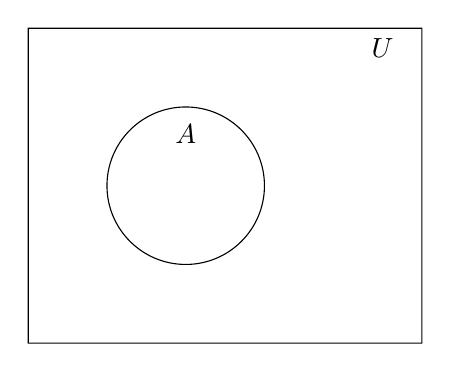
\begin{tikzpicture}[fill=gray]

% outline
\draw (0,0) circle (1) (0,0.9)  node [text=black,below] {$A$}
      (-2,-2) rectangle (3,2)  (2.5,1.5) node [text=black,above] {$U$};
\end{tikzpicture}
}{0in}

\example{
The representation in the above example can be extended to any finite number of sets. If want to represent two disjoint sets, A and B, we can represent them as below.

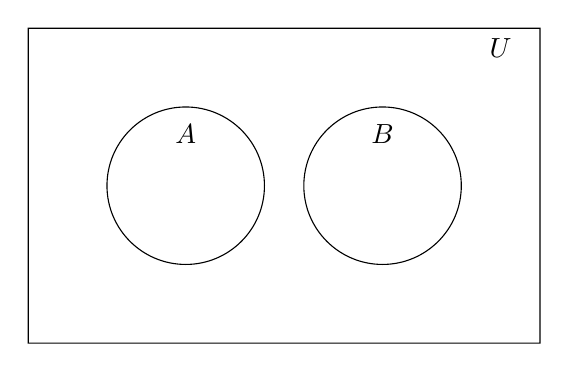
\begin{tikzpicture}[fill=gray]

% outline
\draw (0,0) circle (1) (0,0.9)  node [text=black,below] {$A$}
      (2.5,0) circle (1) (2.5,0.9)  node [text=black,below] {$B$}
      %(5,0) circle (1) (5,1)  node [text=black,above] {$C$}
      (-2,-2) rectangle (4.5,2)
      (4,1.5) node [text=black,above] {$U$};

\end{tikzpicture}

\noindent
The circles do not overlap, to indicate that the sets are disjoint.
Note that $A$ or $B$ or both could actually be empty sets, a bit like looking down into empty paper bags.

}{0in}


\remark{
The power of Venn diagrams is that they make it easy to understand set relations and operations. 
Let's look at a few examples.
}

\example{
If B is a subset of A, that is, if $B \subseteq A$ we can represent this as below.

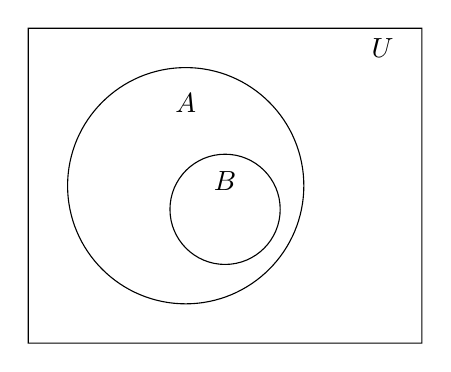
\begin{tikzpicture}[fill=gray]

% outline
\draw (0,0) circle (1.5) (0,1.3)  node [text=black,below] {$A$}
      (0.5,-0.3) circle (0.7) (0.5,0.3)  node [text=black,below] {$B$}
      (-2,-2) rectangle (3,2) (2.5,1.5) node [text=black,above] {$U$};
\end{tikzpicture}

\noindent
Note that it is possible that $B = A$; the blank areas in the diagram may or may not contain points; they may be empty.

}{0in}

\example{
If B is a proper subset of A, we can represent this with a dot outside B, but within A.

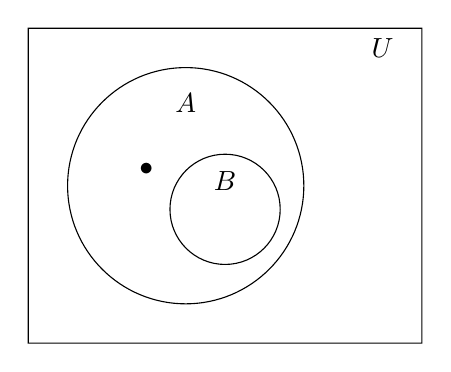
\begin{tikzpicture}[fill=gray]

% outline
\draw (0,0) circle (1.5) (0,1.3)  node [text=black,below] {$A$}
      (0.5,-0.3) circle (0.7) (0.5,0.3)  node [text=black,below] {$B$}
      (-0.5,0) node [text=black,above] {$\bullet$}
      (-2,-2) rectangle (3,2) (2.5,1.5) node [text=black,above] {$U$};
\end{tikzpicture}

\noindent
Now it's clear that every element of $B$ is also an element of $A$, but that there is an element of $A$ that is not an element of $B$.
It could be that $B$ is empty.
}{0in}


\example{
The generic picture of two sets $A$ and $B$ shows them overlapping, but not completely:

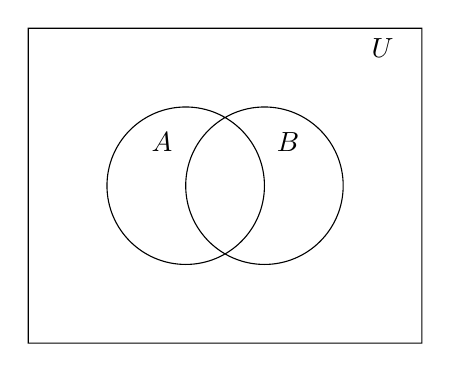
\begin{tikzpicture}[fill=gray]

% outline
\draw (0,0) circle (1) (-0.3,0.8)  node [text=black,below] {$A$}
      (1,0) circle (1) (1.3,0.8)  node [text=black,below] {$B$}
      (-2,-2) rectangle (3,2)  (2.5,1.5) node [text=black,above] {$U$};
\end{tikzpicture}

}{0in}


\example{
To indicate the intersection of $A$ and $B$, we shade $A \cap B$ as below, even if it is possible that the intersection is an empty set:

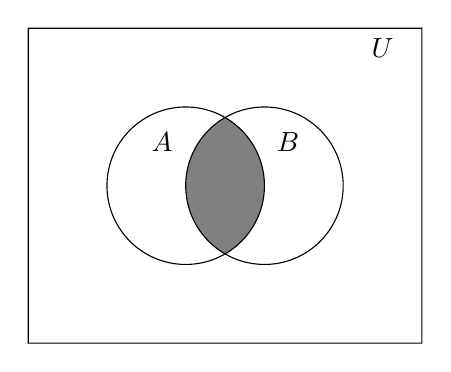
\begin{tikzpicture}[fill=gray]

\scope % A \cap B
\clip (0,0) circle (1);
\fill (1,0) circle (1);
\endscope

% outline
\draw (0,0) circle (1) (-0.3,0.8)  node [text=black,below] {$A$}
      (1,0) circle (1) (1.3,0.8)  node [text=black,below] {$B$}
      (-2,-2) rectangle (3,2)  (2.5,1.5) node [text=black,above] {$U$};
\end{tikzpicture}

}{0in}

\example{
If we know that A and B, are not disjoint, we indicate this by a dot inside the region of their overlap.


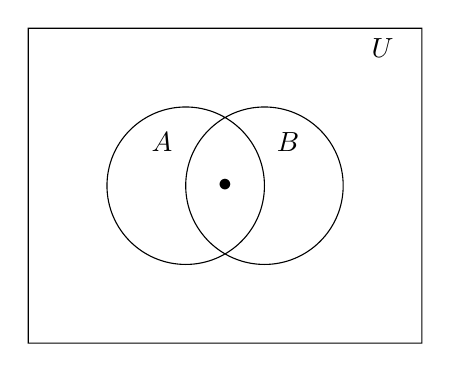
\begin{tikzpicture}[fill=gray]

\scope % A \cap B
\clip (0,0) circle (1);
%\fill (1,0) circle (1);
\endscope

% outline
\draw (0,0) circle (1) (-0.3,0.8)  node [text=black,below] {$A$}
      (1,0) circle (1) (1.3,0.8)  node [text=black,below] {$B$}
      (0.5,-0.2) node [text=black,above] {$\bullet$}
      (-2,-2) rectangle (3,2)  (2.5,1.5) node [text=black,above] {$U$};
\end{tikzpicture}

}{0in}


\example{
For two sets A and B, we represent $A \cup B$ as below:

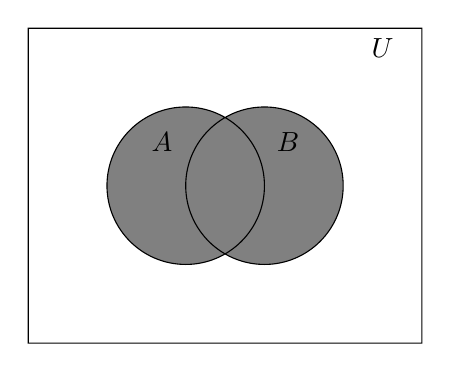
\begin{tikzpicture}[fill=gray]

\scope % A \cap B
\fill (1,0) circle (1);
\fill (0,0) circle (1);
\endscope

% outline
\draw (0,0) circle (1) (-0.3,0.8)  node [text=black,below] {$A$}
      (1,0) circle (1) (1.3,0.8)  node [text=black,below] {$B$}
      (-2,-2) rectangle (3,2)  (2.5,1.5) node [text=black,above] {$U$};
\end{tikzpicture}

}{0in}


\example{
For three sets A, B and C, we draw them to allow for all possible intersections.
We represent $A \cap B \cap C$ as below, even though it may actually be an empty set:

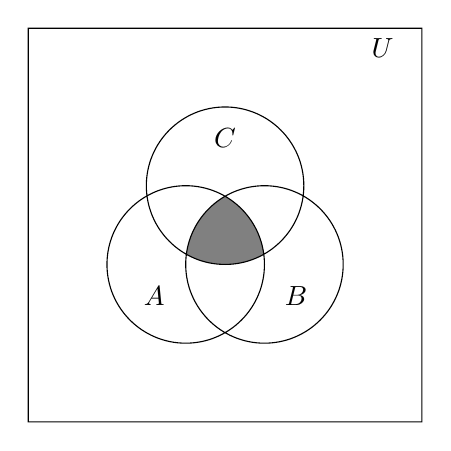
\begin{tikzpicture}[fill=gray]

\scope % A \cap B
\clip (0,0) circle (1);
\clip (0.5,1) circle (1);
\fill (1,0) circle (1);
\endscope

% outline
\draw (0,0) circle (1) (-0.4,-0.4)  node [text=black] {$A$}
      (1,0) circle (1) (1.4,-0.4)  node [text=black] {$B$}
      (0.5,1) circle (1) (0.5,1.6)  node [text=black] {$C$}
      (-2,-2) rectangle (3,3) (2.5,2.5) node [text=black,above] {$U$};
\end{tikzpicture}
}{0in}


\exercise{
For the following questions, represent your answers as Venn diagrams, where possible. If a Venn diagram is not possible, explain why.
\balist{0.8in}
    
\item Make a Venn diagram for sets $A$ and $B$, showing that $A$ and $B$ are disjoint, and shade $A \cup B$.
    
\item Make a Venn diagram for sets $A$, $B$, and $C$, showing that $B$ and $C$ are disjoint.
    Shade the set $(A\cap B)\cup C$.
    
\item Make a Venn diagram for sets $A$, $B$, and $C$, showing that $A \cap B \cap C$ is empty, and shading $(A \cap B) \cup (A \cap C) \cup (B \cap C)$.
    
\item Make a Venn diagram for sets $A$, $B$, and $C$, showing that $A$ and $B$ are not disjoint and that $C \subset B$ but $C$ is disjoint from $A$.  
    
\item Make a Venn diagram for sets $A$, $B$, and $C$, showing that $A \cap B \subset C$, but $C \subset A \cup B$.
    \vspace{8em}
    
    
\elist
}{0.4in}


% =====================================================================
\definition{Set complement}{
The \textbf{complement} of a set A is the set of elements that do not belong to A. 
Therefore, it is every element of the universal set $U$ that is not an element of $A$.
We denote the complement of A as $A^c$ or $A'$. 
Visually, we represent this as:

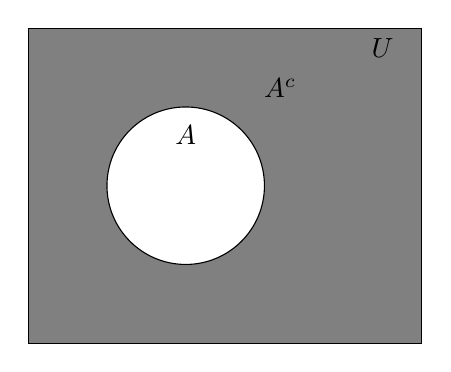
\begin{tikzpicture}[fill=gray]
\scope % A^c
    \filldraw   (-2,-2) rectangle (3,2) (2.5,1.5) node [text=black,above] {$U$};
    \fill[white] (0,0) circle (1);
\endscope
% outline
\draw (0,0) circle (1) (0,0.4)  node [text=black,above] {$A$}
      (1.2,1)  node [text=black,above] {$A^c$};
\end{tikzpicture}

}


\definition{Set difference}{  
The \textbf{difference} of sets A and B is the set of elements which belong to A but not to B. We denote this as $A-B$ or $A \setminus B$. Visually, we represent this by drawing $A$ and $B$ and shading the elements in $A$ but not in $B$.

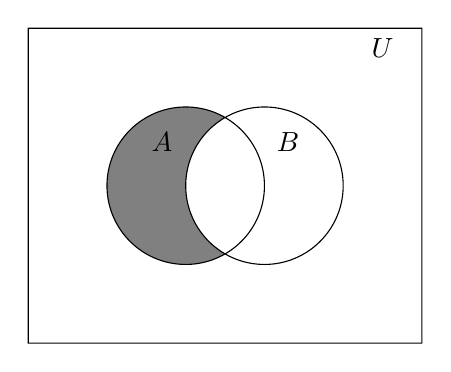
\begin{tikzpicture}[fill=gray]
% left hand
\scope
\clip (-2,-2) rectangle (2,2)
      (1,0) circle (1);
\fill (0,0) circle (1);
\endscope
% right hand
%\scope
%\clip (-2,-2) rectangle (2,2)
      %(0,0) circle (1);
%\fill (1,0) circle (1);
%\endscope
% outline
\draw (0,0) circle (1) (-0.3,0.8)  node [text=black,below] {$A$}
      (1,0) circle (1) (1.3,0.8)  node [text=black,below] {$B$}
      (-2,-2) rectangle (3,2) (2.5,1.5) node [text=black,above] {$U$};
\end{tikzpicture}

%TODO: explain difference of sets as relative complement

}

%TODO: add a remark explaining the concept of relative complement

%\definition{}{
%The \textbf{Cartesian product} of two sets A and B, denoted by A $\times$ B is the set of all ordered pairs $(a,b)$ where a $\in$ A and b $\in$ B. It can be specified using set-builder notation, i.e. $A \times B=\{(a,b) : a\in A$ and  $b\in B\}$.
%}


\exercise{
For the following questions, start by drawing a Venn diagram for sets $A$ and $B$, then shade the desired set or sets.
For more than one set, use different shading for each one.
\balist{0.8in}
    
\item $(A \cap B)^c$, given that $A$ and $B$ are not disjoint.
    
\item $(A^c \cup B^c)$, given that $A$ and $B$ are not disjoint.
    
\item $A^c$ and $A^c \setminus B$.
    
\item Supposing that $B \subset A$, shade in $A \setminus B$. 
       
\elist
}{0.0in}


\yourname

\activitytitle{Operations on sets}{This activity works with set identities and relates them to logic.}

\overview{Sets are absolutely fundamental to mathematics.
This chapter focuses on building up set identities, relationships between sets that are always true.}

\problem{Let $A$ and $B$ be sets.  Show that $(A \cup B)^{c} = A^{c} \cap B^{c}$ by showing set inclusion both ways.  The first part is done for you.  This is one of de Morgan's laws.  Draw a really nice Venn diagram to illustrate.\\
\vspace*{-0.3in}
\begin{itemize}
\item Let $x \in (A \cup B)^{c}$.  
Then $x \notin A \cup B$.  
So $x \notin A$ and $x \notin B$.  
That means that $x \in A^{c}$ and $x \in B^{c}$, and so $x \in A^{c} \cap B^{c}$.  
Since $x$ was arbitrary, $(A \cup B)^{c} \subseteq A^{c} \cap B^{c}$.

\item Let $x \in A^{c} \cap B^{c}$.

\end{itemize}}{1in}

\problem{Let $A$ and $B$ be sets.  Show that $(A \cap B)^{c} = A^{c} \cup B^{c}$ by showing set inclusion both ways.  This is the other one of de Morgan's laws.  Draw a really nice Venn diagram to illustrate.}{2in}

\problem{\label{setsaslogic}Let $A$ and $B$ be sets.  Let $P$ be the logical statement $x \in A$, and let $Q$ be the logical statement $x \in B$.
Use $P$ and $Q$ and logic symbols ($\wedge$ for {\em and}, $\vee$ for {\em or}, $\lnot$ for {\em not}) to translate statements about sets into logic statements:
\blist{0.1in}
\item $x \in A \cup B$ is \blank{1.5in}
\item $x \in A^c$ is \blank{1.5in}
\item $x \in B^c$ is \blank{1.5in}
\item $x \in A^c \cap B^c$ is \blank{1.5in}
\item $x \in (A \cup B)^{c}$ is \blank{1.5in}
\elist
\pagebreak

\noindent
In the white space above and to the right, make a truth table for $P$, $Q$, and each of the other logical statements in the previous problem to establish that $x \in (A \cup B)^c$ is logically equivalent to $x \in A^c \cap B^c$.
Compare the truth values in the columns corresponding to $x \in (A \cup B)^c$ to the Venn diagram you made above.  Explain how they agree.
}{0in}

\problem{Let $A$ and $B$ be sets.  Follow the previous exercise to use a truth table to show that $x \in (A \cap B)^{c}$ is logically equivalent to $x \in A^{c} \cup B^{c}$.  Compare the truth table to the Venn diagram again.}{2in}

\problem{Let $D, E,$ and $F$ be sets.
Use one of de Morgan's laws that you showed above to establish that $(D \cup E \cup F)^c = D^c \cap E^c \cap F^c$.
This proof works by rewriting, not by showing inclusion both ways.
{\bf Hint:} Let $A = D \cup E$ and $B = F$.}{1.5in}

\problem{Let $D, E,$ and $F$ be sets.
Use one of de Morgan's laws to show that $(D \cap E \cap F)^c = D^c \cup E^c \cup F^c$.}{1.5in}

\problem{Let $A, B,$ and $C$ be sets.
Use logical statements $P, Q,$ and $R$ and a truth table to show that $x \in A \cup (B \cap C)$ is logically equivalent to $x \in (A \cup B) \cap (A \cup C)$.  Be sure to define $P$, $Q$, and $R$ at the beginning.}{2in}

\problem{Let $A, B,$ and $C$ be sets.
Show that $A \cup (B \cap C) = (A \cup B) \cap (A \cup C)$ by showing inclusion both ways.
When you encounter a union, use a proof by cases.
For example, if you know that $x \in A \cup B$, one case is that $x \in A$, the other is that $x$ is not in $A$, but $x \in B$.
Organize your writing carefully to make the steps of this argument really clear.}{3in}

\definition{Set difference}{Let $A$ and $B$ be sets.  The {\em set difference} $A \backslash B$ is the set $A \cap B^{c}$, which is all points that are in $A$ but not in $B$.  Draw a Venn diagram to illustrate this definition.}

\definition{Symmetric difference}{Let $A$ and $B$ be sets.  The {\em symmetric difference} of $A$ and $B$ is the set $A \bigtriangleup B = (A \backslash B) \cup (B \backslash A)$.  Draw a Venn diagram to illustrate this definition.}

\problem{Consider again the logical statements from \ref{setsaslogic}.  Write a logical statement that is equivalent to $x \in A \bigtriangleup B$.
Make a truth table with 4 rows, labeled 1, 2, 3, 4, and three columns, one for $x \in A$, one for $x \in B$, and the third for $x \in A \bigtriangleup B$.
Draw a Venn diagram and label the regions in it 1, 2, 3, 4 so that they correspond to the truth table.}{1in}

\problem{Let $A$ and $B$ be sets.  Show that $A \bigtriangleup B = B \bigtriangleup A$ by showing set inclusion both ways.  Draw a nice Venn diagram to illustrate.}{2in}

\problem{Let $A, B,$ and $C$ be sets.  Show that $(A \bigtriangleup B) \bigtriangleup C = A \bigtriangleup (B \bigtriangleup C)$ in three ways.
\blist{0.1in}
\item Draw separate Venn diagrams for the two sets.
\item Show set inclusion both ways.
\item Convert inclusion in $A \bigtriangleup B$, $B \bigtriangleup C$, and other sets to logical statements and use a truth table to show the equality.
\elist
}{0in}

\vfill          % pad the rest of the page with white space

\yourname

\activitytitle{Infinite unions, intersections, and a few other things}{This activity is a prequel to working with infinite unions and intersections.}

\overview{Infinite unions and intersections take a bit of getting used to.  Fortunately, we can understand them with quantifiers, and we can understand intervals with inequalities.}

\definition{Union}{Let $A_1, A_2, \ldots$ be sets, with universe $X$.
The {\em union} of $A_1, A_2, \ldots$, which is denoted $\bigcup_{n=1}^{\infty} A_n$, is all elements of $X$ which are in $A_n$ for some $n = 1, 2, 3, \ldots.$}

\definition{Intersection}{Let $A_1, A_2, \ldots$ be sets, with universe $X$.
The {\em intersection} of $A_1, A_2, \ldots$, which is denoted $\bigcap_{n=1}^{\infty} A_n$, is all elements of $X$ which are in $A_n$ for all $n = 1, 2, 3, \ldots.$}

\problem{Use quantifiers to express what it means that $x \in \bigcup_{n=1}^{\infty} A_n.$\\
{\bf Solution:} $\exists n, x \in A_n$.
In words, there is at least one $n$ for which $x$ is in $A_n$.}{0.5in}

\problem{Work with quantifiers to express what it means that $x \notin \bigcup_{n=1}^{\infty} A_n.$\\
{\bf Hint.} Negate the previous expression and use rules of quantifiers to rewrite it, then rewrite again using complements.}{1.2in}

\problem{Use quantifiers to express what it means that $x \in \bigcap_{n=1}^{\infty} A_n.$}{1.2in}

\problem{Work with quantifiers to express what it means that $x \notin \bigcap_{n=1}^{\infty} A_n.$\\
{\bf Hint.} Negate the previous expression, then rewrite again using complements.}{1.2in}

\stop{Go back to each of the four preceding problems and write a sentence explaining the logic of the expression that you wrote down.}

\problem{de Morgan's law.  Show that $\left( \bigcup_{i \in I} A_i \right)^c = \bigcap_{i \in I} A_i^c$ by writing logical expressions for $x$ being in the set on the left side and for the right side.
Note that here the union is over sets $A_i$ where the index $i$ comes from an index set $I$, but the logic is the same as in the previous problems.
Start by writing a logical expression that means the same thing as $x \in \left( \bigcup_{i \in I} A_i \right)^c$ and work with it until it is a logical expression for $x \in \bigcap_{i \in I} A_i^c$.
When you write the proof this way, you do not need to show containment both ways to show that the two sets are equal.}{1.5in}

\problem{Show that $(3,\infty) \subset [3,\infty)$; these are both intervals on the real number line.
Remember that when you show $\subset$ there are two things to show:  containment, and that there is an element of one set that is not an element of the other.  Solve this problem by letting $x \in (3,\infty)$ and writing that information as the logical statement ``$x > 3$ is true''.}{1.2in}

\problem{Show that $[2,5) \cap (3,7) \subseteq (3,5)$ using inequalities.
Start by letting $x \in [2,5) \cap (3,7)$.}{1in}

\problem{Let $x > 0$.  Show that there exists an integer $n$ such that $0 < \frac{1}{n} < x$.
{\bf Hint:} Look at $\frac{1}{x}$ and round up.
{\bf Another hint:} Suppose that $x = 0.31$. What value of $n$ works?}{1.5in}

\problem{Let $n$ be an integer greater than 0.  Show that $[\frac{1}{n},1] \subseteq (0,1] \subseteq [0,1]$ by working with inequalities.  Then show that $[\frac{1}{n},1] \subset (0,1] \subset [0,1]$ by looking at individual points.}{0in}
\vfill          % pad the rest of the page with white space

\yourname

\activitytitle{Infinite operations on sets}{Unions, intersections, and complements of infinitely many sets}

\overview{We are working with sets of real numbers.  These exercises will give you practice with sets and teach you things about the real numbers as well.}

\problem{Let $A = \bigcup_{n=1}^{\infty} [\frac{1}{n}, 1]$.  
List out the first five sets in this union.  
Draw a picture of them above a number line.  
Make a conjecture about what interval $A$ is equal to, call the new set $B$, then show that $A = B$ by showing containment both ways.
You will need to use this property of real numbers:  if $x > 0$, then there exists a positive integer $n$ with $0 < \frac{1}{n} < x$.}{3in}

\problem{Let $B = \bigcup_{n=0}^{\infty} [n, n^2]$.
List out the first five or more sets in this union.
Draw them on a number line if it helps.
Make a conjecture about how you can write $B$ in a simpler way, call the new set $C$, then prove that $B = C$ by showing containment in both directions.}{3in}

\pagebreak

\problem{For $n = 2, 3, 4, \ldots,$ let $C_n = \{ 2n, 3n, 4n, \ldots \}$.
\blist{1in}
\item Write out the first five of the $C_n$.
\item Let $D = \bigcup_{n=2}^{\infty} C_n$.
Describe the set $D$ in simpler terms, perhaps by writing out the smallest 10 elements of $D$.
\item What is $\N \backslash D$?  Remember that $\N = \{0, 1, 2, 3, \ldots\}$.
\elist
}{0in}

\problem{Let $I$ be a set, and for each $i$ in $I$, let $A_i$ be a set, all subsets of the same universe $X$.
Show de Morgan's law:  $\left( \bigcup_{i \in I} A_i \right)^c = \bigcap_{i \in I} A_i^c$ by showing set containment in both directions.
I hope you will find that it is actually easier to do this for a collection of sets than for two sets.
}{3in}

\problem{Let $E = \bigcap_{n = 1}^{\infty} [0, 1+\frac{1}{n}]$.
List out the first five sets in this union.  
Draw a picture of them above a number line.  
Make a conjecture about what interval $E$ is equal to, call the new set $F$, then prove that $E = F$ by showing containment both ways.

{\bf Hint:} You may want to show that $E \subseteq F$ by showing the logically equivalent statement that $F^c \subseteq E^c$.
This is the same as the contrapositive:  suppose that $y \notin F$, then show that $y \notin E$.
You may find it useful to keep in mind that if $x > 0$, then there exists an integer $n$ for which $0 < \frac{1}{n} < x$.
}{3in}

\problem{Let $F = \bigcup_{r \in \Q} (r-\frac{1}{10}, r+\frac{1}{10})$.
Here, $\Q$ is the set of all rational numbers.
Make a conjecture about a simpler way to describe the set $F$, then prove your conjecture by showing set containment both ways.}{3in}

\problem{Let $G = \bigcup_{k \in \Z} (k, k+1)$.
\blist{1in} 
\item Draw out some of the intervals here.
\item Make a conjecture about what set $G$ is.
\item Use one of de Morgan's laws to re--express $G^c$ as an intersection.
Does that help?
\item What is easier to describe, or to think of, $G$ or $G^c$?
Give the simplest description.
\elist}{0in}

\problem{Let $a < b$.  Show that $\bigcup_{n=1}^{\infty} [a, b-\frac{1}{n}] = [a,b)$.  Draw pictures, then show set inclusion both ways.  Is there a problem if $b - \frac{1}{n} < a$?}{2in}

\problem{Let $a < b$.  Show that $\bigcap_{n=1}^{\infty} [a,b+\frac{1}{n}) = [a,b]$.  Draw pictures, then show set inclusion both ways.}{2in}


\vfill          % pad the rest of the page with white space

\yourname

\activitytitle{Set theory practice}{More practice working with sets}

\overview{Write really detailed proofs with crystal clear logic.  In particular, when showing that $A \subseteq B$, start with ``Let $x \in A$,'' show that $x$ is in $B$, and then say, ``Since $x \in A$ was arbitrary, $A \subseteq B$.''}

\show{Let $A, B$, and $C$ be sets.
Suppose that $A \subseteq B$ and $B \subseteq C$.
Show that $A \subseteq C$.
{\bf Note:} This {\em shows} transitivity but it does not {\em use} transitivity.}{1in}

\show{Let $A, B$, and $C$ be sets.
Suppose that $A \subset B$ and $B \subset C$.
Show that $A \subset C$.
{\bf Note:} Here we have strict set inclusion, so you will need to show that $A$ is not equal to $C$.
}{1in}

\show{Let $A, B$, and $C$ be sets.
Show that $C \subseteq A$ and $C \subseteq B$ if and only if $C \subseteq A \cap B$.
{\bf Note:}  ``If and only if'' means there are two things to show:
\blist{1in}
\item Suppose that $C \subseteq A$ and $C \subseteq B$.  Show that $C \subseteq A \cap B$.
\item Suppose that $C \subseteq A \cap B$.  Show that $C \subseteq A$ and $C \subseteq B$.
\elist
}{1in}

\show{Let $A$ and $B$ be sets.
Show that $A \cap B = B$ if and only if $B \subseteq A$.
}{2in}

\show{Let $A_1, A_2, A_3, \ldots$ and $B_1, B_2, B_3, \ldots$ be sets.
Suppose that $A_n \subseteq B_n$ for all $n = 1, 2, 3, \ldots$.
Show that $\bigcap_{n=1}^{\infty} A_n \subseteq \bigcap_{n=1}^{\infty} B_n$}{2in}

\show{Let $A_1, A_2, A_3, \ldots$ and $B_1, B_2, B_3, \ldots$ be sets.
Suppose that $A_n \subseteq B_n$ for all $n = 1, 2, 3, \ldots$.
Show that $\bigcup_{n=1}^{\infty} A_n \subseteq \bigcup_{n=1}^{\infty} B_n$}{2in}

\show{Let $A$ and $B_1, B_2, B_3, \ldots$ be sets.
Suppose that $A \subseteq \bigcap_{n=1}^{\infty} B_n$.  
Show that $A \subseteq B_n$ for all $n = 1, 2, 3, \ldots$.
Start the proof with ``Let $n \geq 1$ be an integer'' and be sure to end the proof by generalizing over $n$.
The second step in the proof is ``Let $x \in A$.''}{0in}

\vfill          % pad the rest of the page with white space

\yourname

\activitytitle{The power set and the Cartesian product}{Useful constructions with sets.}

\overview{The power set is our first example of thinking hard about collections of sets.  The Cartesian product is used often when you want ordered pairs or ordered triples of numbers or other objects.}

\problem{Write out the members of the following power sets.  It may be helpful to do \#3, \#4, then \#2, \#1, and finally \#5.
\blist{0.1in}
\item $S = \emptyset$.  ${\cal P}(S) = $
\item $S = \{ 1 \}$.  ${\cal P}(S) = $
\item $S = \{ 1,2 \}$.  ${\cal P}(S) = $
\item $S = \{ 1,2,3 \}$.  ${\cal P}(S) = $
\item $S = \{ 1,2,3,4 \}$.  ${\cal P}(S) = $
\item $S = \{ 1,2,3,4,5 \}$.  ${\cal P}(S) = $
\elist
}{0in}

\question{If $S$ has $n$ elements, how many members will ${\cal P}(S)$ have?  Explain as well as you can.}{1in}

\problem{Write the appropriate symbol between the entities, or mark the statement as true or false.  Give an explanation for anything that is not obvious enough.
\blist{0.0in}
\item $ 1 \quad\quad {\cal P}(\{ 1, 2, 3 \})$
\item $[3, 10] \quad\quad \Z$
\item $[3, 10] \quad\quad \R$
\item $\Q \quad\quad \R$
\item $\Q \quad\quad {\cal P}(\R)$
\item $[3, 10] \quad\quad {\cal P}(\R)$
\item $\N \quad\quad \R$
\item $\emptyset \quad\quad \R$
\item $\emptyset \quad\quad {\cal P}(\R)$
\item $\{ \emptyset \} \subseteq A$?
\item $\emptyset \subset {\cal P}(A)$?
\elist
}{0.0in}

\question{Suppose that $S$ is a set.  Then ${\cal P}(S)$ is also a set, but if we let $A \in {\cal P}(S)$, then $A$ is also a set.
Explain how this can be.
What is the relationship between $A$ and $S$?}{1.5in}

\problem{Let $I$ be a set, and for each $i$ in $I$, let $B_i$ be a set.
Show that ${\cal P}\left( \bigcap_{i \in I} B_i \right) = \bigcap_{i \in I} {\cal P}(B_i)$.\\
Let $A$ be an element of the set on the left-hand side.  Notice that $A$ is a set.  Argue that it is an element of the set on the right-hand side.
\vspace{1in}
Let $A$ be an element of the set on the right-hand side \ldots}{1in}

\problem{
\blist{0.75in}
\item Sketch the Cartesian product $A = [1,3] \times [2,5]$.
\item Sketch the Cartesian product $B = [2,4] \times [1,3]$.
\item Sketch the intersection $A \cap B$.
\item It seems that $A \cap B$ is also a Cartesian product.  Identify the sets whose product is $A \cap B$.
\item What is $([1,3] \cap [2,4]) \times ([2,5]\cap[1,3])$?
\elist
}{0.0in}

\vfill          % pad the rest of the page with white space

\yourname

\activitytitle{Relations}{Often treated as the little brother to functions, relations have unsuspected depth.}

\overview{You are already familiar with a number of relations, including $<, \leq, =, \geq,$ and $>$ for real numbers, plus $\subset$, $\subseteq$, and $=$ for sets.  Many other relations can be defined.  The most useful ones are called equivalence relations; they are analogous to equality for numbers and for sets.  They partition the space into equivalence classes, which are very useful in a number of ways.}

\definition{Relation}{A {\em relation} on a set $X$ is a subset $S$ of $X \times X$.}

\notation{Suppose that $S$ is a relation on a set $X$.
That is, suppose that $S$ is a subset of $X \times X$, which means that $S$ is a set of points of the form $(x,y)$, where $x \in X$ and $y \in X$.
Rather than write $(x,y) \in S$, we usually write $x \sim y$.
How to read this out loud?  There is no perfect solution.  I would suggest that you read it as ``$x$ tilde $y$'' because $\sim$ is the tilde that appears above the n in some Spanish words.}

\problem{
You are going to write out the subsets of $\{1, 2, 3, 4\}$ and then draw arrows between them to indicate the proper subset relation.  You might want to lay the sets out in a nice order to make the arrows easy to draw and to read.
What is the set $X$ on which this relation is defined?
}{2in}

\definition{Reflexive}{A relation $\sim$ is {\em reflexive} if $x \sim x$ for all $x$ in $X$.}

\definition{Symmetric}{A relation $\sim$ is {\em symmetric} if $x \sim y$ implies $y \sim x$.}

\definition{Transitive}{A relation $\sim$ is {\em transitive} if $x \sim y$ and $y \sim z$ implies $x \sim z$.}

\note{Sometimes people have a hard time remembering the words reflexivity, symmetry, and transitivity.  Notice that they are in alphabetical order, and that they involve 1, 2, or 3 objects at a time, respectively.}

\definition{Equivalence relation}{A relation $\sim$ is called an {\em equivalence relation} if it is reflexive, symmetric, and transitive.  Note that equality is an equivalence relation on the set of real numbers.}

\definition{Equivalence class}{Suppose that $\sim$ is an equivalence relation.  Fix $x$ in $X$.  The set of all elements $y$ for which $x \sim y$ is called the {\em equivalence class containing $x$}.}


\problem{Let $X = \Z^+$ and say that $x \sim y$ if $y$ is divisible by $x$.
People often write $x | y$ for this relation and say that $x$ divides $y$.
\blist{0.8in}
\item Check whether this relation is reflexive.  If so, prove that it is, starting with ``Let $x \in \Z^+$.''  If not, give a counterexample.
\item Check whether this relation is symmetric.  If so, prove that it is, starting with ``Let $x, y \in \Z^+$ and suppose that $x \sim y$.''  If not, give a counterexample.
\item Check whether this relation is transitive. If so, prove that it is, starting with  ``Let $x, y, z \in \Z^+$ and suppose that $x \sim y$ and $y \sim z$.''  If not, give a counterexample.
\item Thinking of the relation as a set of ordered pairs, write out ten different ordered pairs satisfying the relation, and graph them on the $xy$ plane.
\elist
}{0.5in}

\problem{Consider all cities in the US that have population over 30,000.
For each of the following relations, determine whether they are reflexive, symmetric, and/or transitive.  Provide a counterexample for any property that fails to hold.  If all three hold, the relation is an equivalence relation.  In that case, identify the equivalence classes and tell how many such classes there are.
\blist{1.2in}
\item Say that $x \sim y$ if the names of cities $x$ and $y$ start with the same letter.
\item Say that $x \sim y$ if $x$ and $y$ are in the same state.
\item Say that $x \sim y$ if cities $x$ and $y$ are within 50 miles of each other.
\elist
}{1.2in}

\problem{Let $X$ be the set of all English words.
Say that $x \sim y$ if the letters in $x$ and $y$ appear on the same number keys on a cell phone, in the same order.
For example, BAR $\sim$ CAP.
\blist{0.5in}
\item Check whether this relation is reflexive.
\item Check whether this relation is symmetric.
\item Check whether this relation is transitive.
\item If all three properties hold, describe the equivalence classes, and tell what the equivalence class of BAR is.
\elist}{0.5in}


\problem{
Let $X = \Z$.
Say that $x \sim y$ if $x$ and $y$ has the same remainder as $y$ when they are divided by 3.
Then, for example, $13 \sim 19$ and $9 \sim 27$.
\blist{0.5in}
\item Show that this relation is reflexive, symmetric, and transitive.
Do this in general, starting with ``Let.''
\vspace*{0.8in}
\item Describe all elements of the equivalence class containing 0.
\item Describe the other equivalence classes.  How many are there?
\elist
}{0.3in}

\problem{Consider the set $X$ of all non--zero 3--dimensional vectors.
For $\vec{a}$ and $\vec{b}$ in $X$, say that $\vec{a} \sim \vec{b}$ if there exists a constant $c$ for which $\vec{a} = c \vec{b}$.
\blist{0.8in}
\item Show that this relation is reflexive, starting with ``Let.''  Tell what $c$ is.
\item Show that this relation is symmetric.  You will need two values of $c$.
\item Show that this relation is transitive.  Here there will be three values of $c$.
\item This is an equivalence relation.  Describe the equivalence classes.  The collection of all equivalence classes is called {\em projective space}.
\item Could you use the angle between lines to define a distance between equivalence classes?  What would the maximum distance be?
\elist}{0in}

\problem{Consider the set of all English words.
Say that $x \sim y$ if one can be obtained from the other by changing exactly one letter.
For example, BAT $\sim$ CAT but BAT $\nsim$ CAR.
Check whether this relation is reflexive, symmetric, and/or transitive.
Provide counterexamples if necessary.}{1in}

\problem{Consider the set of all functions on the real line.
That is, consider the set of all $f : \R \to \R$.
Say that $f \sim g$ if $f$ and $g$ are equal except at a finite number of points.
For example, if $f(x) = x^2$ and $g(x) = \left\{ \begin{array}{cl} x^2, & x \ne 0 \\ 5, & x = 0 \end{array} \right.,$ then $f \sim g$.
Show that this is an equivalence relation.
How can you describe the equivalence classes?}{1.5in}

\note{Problems 10.1 and 10.3 from Daepp and Gorkin\DGreference~are particularly good at this stage in the course.}
\vfill          % pad the rest of the page with white space

\activitytitle{Homework problems, week 12}{Due on (put date here).}

Write up solutions of each of the problems below.
They are designed to be straightforward problems.
The goal is to come as close to perfection in your solutions as you can.
\begin{itemize} \itemsep 1pt
\item Do not take shortcuts.
\item If you need to show that something is true for all $n$, or for all $x,y$, start the proof with ``Let \ldots''
\item If you need cases, explain what the cases are and why they cover all the possibilities.
\item If you are doing a proof by contradiction, start that part by saying ``Assume \ldots''
\item If you are doing a proof by contrapositive, tell what $P$ and $Q$ are, and that you will be showing that $\lnot Q$ implies $\lnot P$.
\item Take small steps in each proof, and explain each step.
\item Follow good form.
\item If your proof started with ``Let \ldots'' it will probably end by saying ``We made no further assumption \ldots''
\end{itemize}
Here are the problems to do.  You can write them in your notebook or on separate paper.
\blist{0.1in}
\item Show that if $n$ is an integer and $7n$ is odd, then $n$ is odd.
{\bf Hint:} Be clear what facts you are using about even and odd numbers.

\item Without consulting your book or your notes, prove that $\sqrt{2}$ is irrational.
I mean it.  
Do this from memory.
You should be able to write a very nice proof, with no missing steps.

\item Let $x$ and $y$ be real numbers, and suppose that the product $xy$ is irrational.
Show that either $x$ or $y$ (or both) must be irrational.
{\bf Hint:} You can do this.  Be patient, think about it.

\item Let $A = \{2k+1 : k \in \Z\}$ and let $B = \{ 2m-11 : m \in \Z \}$.
Show that $A = B$ by showing containment both ways.
{\bf Hint:}  Use good form!

\item Let $A = \{ (x,y) \in \R^2 : y = 5x/7 - 2/7 \}$ and $B = \{ (x,y) \in \R^2 : 5x - 7y = 2 \}$.
Show that $A = B$ by showing containment both ways.

\item Let $A = \{ m \in \Z : m = 15k$ for some $k \in \Z \}$, let $B = \{ m \in \Z : m = 35j$ for some $j \in \Z \}$, and let $C = \{ m \in \Z : m = 105n$ for some $n \in \Z \}$.
Show that $A \cap B = C$ by showing containment both ways.
One direction is easier than the other.
Label one of them ``the easy direction'' and the other ``the hard direction''.
{\bf Hint:} Yes, we worked on a problem just like this in class.
Don't go back and find it, work through this one on your own.
{\bf Another hint:}  In the hard direction, you should come to something like $3k = 7j$ where $j$ and $k$ are integers.
You will need to conclude that $j$ is a multiple of 3.
If you are up for the challenge, show this using the division algorithm.
Don't use any ideas about prime factorization.
\elist

\vfill          % pad the rest of the page with white space

\yourname

\activitytitle{Deriving properties of inequalities}{We can define the $<$ relation for real numbers and establish its properties.}

\overview{In this activity, we back up to the point after the real numbers have been constructed, but before subtraction and inequalities have been defined.  We define the $<$ relation and prove a number of useful properties that it satisfies.  Since the $>$ relation is so similar, we will not define it or show its properties.}

\remark{Most of us first learned numbers by counting, using 1, 2, 3, \ldots, which we will call {\em positive integers}.
Later, we learned about addition of positive integers and multiplication of positive integers.
Both operations give back positive integers; we say that the set of positive integers is {\em closed} under addition and multiplication.
Later, we learned about zero, negative numbers, rational numbers, and real numbers.
It is not always made clear, but the negative integers can be constructed from the positive integers, the rationals from the integers, and the reals from the rationals.
In this activity, we assume that the real numbers have been constructed and have been shown to have their usual algebraic properties, and work from there to prove some basic (and very familiar) facts.}

\note{\label{realnumberproperties}Let $\R$ denote the set of real numbers, and denote addition and multiplication of real numbers in the usual ways.
{\bf Addition} has these properties:  commutativity ($a+b = b+a$), associativity ($a + (b+c) = (a+b) +c$), additive identity (there exists a unique real number called 0 for which $a + 0 = a$ for all $a \in \R$), and additive inverse (for each number $a$ in $\R$, there exists a unique real number $-a$ for which $a + (-a) = 0$).
{\bf Multiplication} has these properties:  commutativity ($ab = ba$), associativity ($a(bc) = (ab)c$), multiplicative identity (there exists a unique real number called 1, with $1 \ne 0$, such that $a\cdot 1 = a$ for all $a$ in $\R$), multiplicative inverse (for each $a$ in $\R$ with $a \ne 0$, there exists a unique number called $a^{-1}$ for which $a \cdot a^{-1} = 1$.
{\bf Addition and multiplication} are related by the distributive property: ($(a+b)c = ac + bc$).}

\note{In this activity, subtraction is not defined, so be careful not to use it!}

\show{Let $a$ be a real number.  Justify each line in the following proof to show that $0 \cdot a = 0$.
\beqnarray{-0.1in}
  a + (-a) &=& 0 \qqqq\qqqq\qqqq\qqqq ~\\
  1 \cdot a + (-a) &=& 0 \\
  (0+1) \cdot a + (-a) &=& 0 \\
  (0 \cdot a + 1 \cdot a) + (-a) &=& 0 \\
  (0 \cdot a + a) + (-a) &=& 0 \\
  0 \cdot a + (a + (-a)) &=& 0 \\
  0 \cdot a + 0 &=& 0 \\
  0 \cdot a &=& 0
\eeqnarray{-0.5in}
}{0.0in}

\show{People sometimes ask if the additive inverse $(-a)$ is the same as the product $(-1)\cdot a$, where $(-1)$ is the additive inverse of 1.
It's true, and here is how you show it; fill in steps and write the justifications at the right side of each line.
\beqnarray{-0.1in}
  a + (-1)\cdot a &=& 1\cdot a + (-1) \cdot a \qqqq\qqqq\qqqq\qqqq ~ \\
                  &=& (1 + (-1)) \cdot a \\
                  &=&  \\
                  &=& 0,
\eeqnarray{-0.5in}
This shows that $(-1) \cdot a$ is the additive inverse of $a$, because that number is unique.}{0in}

\show{You might think that it is obvious that $(-1)(-1) = 1$, where $(-1)$ is the additive inverse of 1, but this takes a few steps.
Fill in steps and write justifications.
\beqnarray{-0.1in}
(-1) + (-1)(-1) &=& (-1)(1) + (-1)(-1) \qqqq\qqqq\qqqq\qqqq ~\\
                &=& (-1)(1 + (-1)) \\
                &=& \\
                &=& 0
\eeqnarray{-0.25in}

\noindent
Why does this show that $(-1)(-1)$ is the additive inverse of $-1$?}{0in}

\show{The additive inverse of a sum works out nicely.
Let $a$ and $b$ be real numbers and think about the additive inverse of $a+b$.
Write justifications to the right of each statement.
\beqnarray{-0.1in}
-(a+b) &=& (-1)(a+b) \\
       &=& (-1)(a) + (-1)(b) \\
       &=& (-a) + (-b)
\eeqnarray{-0.5in}
}{0in}

\show{Let $a \in \R$.  The statement $-(-a) = a$ is just a statement about additive inverses.  Prove that it is true.}{0.4in}

\definition{Positive real numbers\label{positivereals}}{By construction, the real numbers have a subset $\Rp$, called the {\em positive real numbers,} for which:
\balist{0.3in}
\item If $a,b \in \Rp$, then $a + b \in \Rp$.  ($\Rp$ is closed under addition.)
\item If $a,b \in \Rp$, then $a\cdot b \in \Rp$.  ($\Rp$ is closed under multiplication.)
\item For every real number $a$, either $a \in \Rp$ or $(-a) \in \Rp$ or $a = 0$.  Exactly one of the three happens.
\ealist
\vspace{0.2in}

\noindent
Note that the positive real numbers are exactly analogous to the positive integers that you learned first.
We can't use interval notation to write what $\Rp$ is, because intervals are defined in terms of inequalities, and we have not defined inequalities yet!
}

\exercise{
Under each property in \ref{positivereals}, write a sentence that states it in plain English
}{0in}

\show{Let $a \in \R$ and suppose that $a \ne 0$.
Show that $a\cdot a \in \Rp$, justifying each step, citing previous definitions or results by number.
{\bf Hint:} Use a proof by cases, using the two remaining cases in \ref{positivereals}c.
For future reference, this gives us a new way to show that a number is in $\Rp$.

\balist{0.3in}
\item Suppose that $a \in $ \blank{0.5in}.
\item Suppose that $(-a) \in $ \blank{0.5in}.
\elist
}{0.4in}

\show{Show that $1 \in \Rp$.  Justify each step.}{0.5in}

\show{Show that $(-1) \notin \Rp$.
{\bf Hint:} Pretend for a minute that $(-1) \in \Rp$ and use \ref{positivereals}a.}{0.5in}

\definition{Less than}{\label{lessthan}Let $a$ and $b$ be real numbers.  We write that $a < b$ if $b + (-a) \in \Rp$.}

\note{All of the following problems rely on  Definition \ref{lessthan}, so you will use it over and over.
Note that $>$ has not been defined yet, so be careful not to use it.}

\show{Show that $-1 < 0$.}{0.5in}

\show{Show that $1 < 1$ is not true.
Thus, the $<$ relation is not reflexive.
Justify each step, citing previous results by number.
}{0.7in}

\show{Show that $0 < 1$.

\vspace{0.5in}
\noindent
Show that $1 < 0$ is not true.
Thus, the $<$ relation is not symmetric.}{0.5in}

\show{Show that the $<$ relation on $\R$ is transitive.
Follow good form by first letting $a, b, c$ be real numbers and supposing that $a < b$ and $b < c$, then showing $a < c$.
Justify each step by number.
In this proof, you are likely to use the fact that $(-b) + b = 0$, which is the additive inverse property.}{0.9in}

\show{Let $a,b \in \R$ and suppose that $a < b$.
Show that $-b < -a$.
Justify each step.
}{0.7in}

\show{Let $a, b, c \in \R$.  Suppose that $a < b$.  Show that $a+c < b+c$.
Justify each step.
}{0.7in}

\show{Let $a, b, c, d \in \R$.  Suppose that $a < b$ and $c < d$.  Show that $a+c < b+d$.
Justify each step.
}{0.9in}

\show{Let $a, b, c$ be real numbers.  Suppose that $a < b$ and $0 < c$.
Show that $ac < bc$.
}{0.7in}

\show{Let $a, b, c$ be real numbers.  Suppose that $a < b$ and $c < 0$.
Show that $bc < ac$.
}{0.9in}

\show{Let $a,b \in \R$ and suppose that $0 < a$ and $b < 0$.
Use a previous result to show that $ab < 0$.}{0.7in}

\show{Let $a \in \R$ and suppose that $0 < a$.
Show that $0 < a^{-1}$.
Here $a^{-1}$ is the multiplicative inverse of $a$.
{\bf Hint:}  This one take a bit more effort than the previous ones.
Note that division has not been defined yet, so just use addition and multiplication.}{0.9in}

\show{Let $a,b \in \R$ and suppose that $0 < a$ and $a < b$.
Show that $b^{-1} < a^{-1}$.}{0.9in}

\vfill          % pad the rest of the page with white space




\yourname

\activitytitle{Absolute value and related functions}{A careful development of the properties of the absolute value function.}

\overview{The absolute value function is easy to understand for numbers like 9 and $-13$, but it's harder to show its properties because our intuition works so hard to see all variables as having positive values.
In this activity, we will not use the standard notation for the absolute value function and will have to keep our intuition at bay.
We will instead rely completely on the definition.
{\bf When you use a property of inequalities, cite it by number.}}

\definition{Absolute value}{The function $f : \R \to \R$ defined by
\[
    f(x) = \left\{ \begin{array}{cl} x, & \mbox{if $x \geq 0$} \\
                          -x, & \mbox{if $x < 0$} \end{array} \right.
\]
is called the {\em absolute value} function.}

\notation{In this activity, do not use the standard notation for absolute value, not even once.
Every time you work with the absolute value function, use and cite the definition.}

\show{\label{absofproduct}Show that $f(ab) = f(a) f(b)$ for all real numbers $a$ and $b$.
Follow the model.\\

Let $a$ and $b$ be real numbers.
There are four cases.
\blist{0.5in}
\item Suppose that $a \geq 0$ and $b \geq 0$.  Then $ab \geq 0$ so $f(ab) = ab$ and $f(a) = a$ and $f(b) = b$, so $f(ab) = ab = f(a)f(b)$.
\item Suppose that $a \geq 0$ and $b < 0$.
\item Suppose that $a < 0$ and $b \geq 0$.
\item Suppose that $a < 0$ and $b < 0$.
\elist
In each case, we see that \blank{2in}.
We made no further assumptions about \blank{1in}, thus \blank{3in}.}{0in}

\show{Following the model above, show that $f(f(a)) = f(a)$ for all real numbers $a$.}{1in}

\show{Show that $f(-a) = f(a)$ for all real numbers $a$.}{1in}

\show{Show that $f(a-b) = f(b-a)$ for all real numbers $a$ and $b$.}{1in}

\show{Show that $f(a) \geq 0$ for all real numbers $a$.}{1in}

\show{Follow the model in \ref{absofproduct} to show that $f(a+b) \leq f(a) + f(b)$ for all real numbers $a$ and $b$.
When $a$ and $b$ have different signs, consider two cases, $a+b \geq 0$ and $a+b < 0$.
You will probably want to show that if $b < 0$, then $b < -b$.
Make a good, solid argument using transitivity of $<$.}{3in}

\show{Show that for real numbers $a$ and $b$, $f(a) \leq b$ if and only if $-b \leq a \leq b$.
Remember that an ``if and only if'' proof has two directions.
In both directions, you will have to consider two cases, $a \geq 0$ and $a < 0$.
Note that the statement $-b \leq a \leq b$ is equivalent to ($-b \leq a$ and $a \leq b$).}{3in}

\show{Show that for all real numbers $a$ and $b$, $f(a) \geq b$ if and only if ($a \geq b$ or $a \leq -b$).}{2in}

\show{Show that for all real numbers $a$ and $b$, $f(a) \leq f(a-b) + f(b)$. {\bf Hint:} Look at $f((a-b)+b)$.}{1in}

\show{Show that for all real numbers $a$ and $b$, $f(a) - f(b) \leq f(a-b)$ and also $f(b)-f(a) \leq f(b-a)$.}{1in}

\show{Show that for all real numbers $a$ and $b$, $f(a-b) \geq f(f(a)-f(b))$.}{1in}

\definition{Minimum function}{The function $h : [0,\infty) \to \R$ defined by 
\[
    h(x) = \left\{ \begin{array}{cl} x, & \mbox{if $x \leq 1$} \\
                                     1, & \mbox{if $x > 1$} \end{array} \right.
\]
can be called the minimum function.}

\show{Show that for all real numbers $a$, $h(a) = 0$ if and only if $a = 0$.}{1.5in}

\show{Show that if $a \leq b$, then $h(a) \leq h(b)$.}{1.5in}

\show{Show that if $h(a) < h(b)$, then $a < b$.}{1.5in}

\show{Show that for all real numbers $a$ and $b$, $h(a+b) \leq h(a) + h(b)$.
{\bf Hint:}  Use a proof by cases.  But what are the cases?}{0in}

\vfill          % pad the rest of the page with white space

\include{pigeonhole_principle}
\yourname

\activitytitle{Functions}{One-to-one, onto and bijective functions}

\overview{You are comfortable working with functions already. There are various ways of describing functions. Here you will learn the formal definition of a function.}

\definition{Function}{Let $X$ and $Y$ be sets. A function $f$ from $X$ to $Y$ is a relation from $X$ to $Y$ that satisfies:
\begin{enumerate}
\item for each $x \in X$ there is a $y \in Y$ such that $(x,y)\in f$, and
\item if $(x,y)\in f$ and $(x,z)\in f$, then $y=z$.
\end{enumerate}
The set $X$ is called the domain of $f$ and the set $Y$ is called the codomain of $f$.}

\notation{We write $f:X\rightarrow Y$ to describe a function $f$ from $X$ to $Y$ and we write $f(x)=y$ instead of $(x,y)\in f$.}

\definition{Injective Functions} {Let $X$ and $Y$ be sets and let $f:X \rightarrow Y$ be a function. The function $f$ is said to be injective or one-to-one if whenever $x_1,x_2 \in X$ are such that $x_1\neq x_2$ then $f(x_1) \neq f(x_2)$.}

\definition{Surjective Functions} {Let $X$ and $Y$ be sets and let $f:X \rightarrow Y$ be a function. The function $f$ is said to be surjective or onto if for each $y\in Y$ there exists an $x\in X$ such that $f(x)=y$.}

\definition{Bijective Functions}{Let $X$ and $Y$ be sets and let $f:X \rightarrow Y$ be a function. The function $f$ is said to be bijective if it is both injective and surjective.} 

\example{Let $X=\{Monday, \diamondsuit, \sqrt{\pi}, purple\}$ and $Y=\{\alpha, \heartsuit, fun\}$ be sets and define the relation $f$ from $X$ to $Y$ by $f=\{(Monday, fun), (\diamondsuit, \alpha), (\sqrt{\pi}, fun), (purple, fun)\}$. Draw a diagram to illustrate the relation. Is the relation $f$ a function? Prove your answer by using the definition.} {2in}

\problem{Let $X=\{Cleveland, Chicago, Los Angeles, Miami \}$ be a set of American cities and let $Y=\{Cavaliers, Heat, Lakers, Bulls, Clippers\}$ be a set of NBA teams. 

a) Provide an example of a relation that is a function from $X$ to $Y$ and draw a diagram to illustrate your example.
\vspace{2in}

b) Provide an example of a relation from $X$ to $Y$ that is not a function and draw a diagram to illustrate your example.
\vspace{2in}

c) Provide  an example of an injective function from $X$ to $Y$. Draw a diagram to illustrate your example.
\vspace{2in}

d) Show that there are no surjective functions from $X$ to $Y$.}{2in}

\note{The next problem states an equivalent definition for injectivity. This definition is very useful when proving that a function is injective.}
\problem{Let $X$ and $Y$ be two sets and let $f:X \rightarrow Y$ be a function. Then $f$ is injective if and only if for all $x_1, x_2 \in X$ such that $f(x_1)=f(x_2)$ we have $x_1=x_2$.}{1in}

\problem {Let $f:\N \rightarrow \N$ be a function defined by $f(n)=2n+1$. Show that the function $f$ is injective but not surjective.
 
{\bf Hint:} Use the previous problem to prove injectivity. In order to prove that $f$ is not surjective you need to find an $m\in \N$ which cannot be written as $2n+1$.}{2in}

\problem {Let $f:\N \rightarrow \Z$ be a function defined by 
$$
   f(n) = \left\{
     \begin{array}{lr}
       \frac{n}{2},       & \text{if } n \text{ is even} \\
       \frac{-(n+1)}{2},  & \text{if } n \text{ is odd} 
     \end{array}
   \right.
$$ 
Show that $f$ is a bijective function. 

{\bf Hint:} To show that $f$ is injective let $n_1, n_2 \in \N$ be such that $f(n_1)=f(n_2)$ and look at all the possible cases according to the parity of $n_1$ and $n_2$. 

To prove the surjectivity let $m\in \Z$. Consider the two possible cases; one when $m\geq 0$ and the other one when $m<0$. Then in each case find an $n \in \N$ such that $f(n)=m$.}{3in}

\vfill

\yourname

\activitytitle{Square roots of prime numbers are irrational}{This is a classic example of proof by contradiction.}

\overview{Most students are familiar with the fact that $\sqrt{2}$ is irrational, but few can prove it.  Having read a proof of this fact in your textbook or online, the starting point is to re-create the proof from memory, then to move on to showing that $\sqrt{3}$ is irrational.  The proof is similar and yet different.}

\definition{Irrational\label{irrational}}{A real number is said to be {\em irrational} if it cannot be written as the quotient of two integers.}

\prove{Prove that $\sqrt{2}$ is irrational by contradiction.  The proof begins with ``Assume that $\sqrt{2}$ can be written as $\frac{p}{q}$ where $p$ and $q$ are integers.''
Argue to a contradiction.}{3in}

\note{If you are new to proof by contradiction, you might prefer to start the previous proof by writing ``Let's pretend for a minute that $\sqrt{2}$ can be written as $\frac{p}{q}$ where $p$ and $q$ are integers.''  This makes it extra clear that you don't really believe that $\sqrt{2}$ is rational, you are just exploring what would happen if that were true.  When you arrive at a contradiction, you realize it's time to stop pretending; $\sqrt{2}$ must be irrational.}

\show{A key step in the proof is that if $n$ is an integer and $n^2$ is even, then $n$ is even.  You may have already shown this, using a proof by contradiction (which begins, ``Assume that $n$ is odd.'') or a proof by contrapositive (which begins, ``Let us show the contrapositive, that if $n$ is not odd, then $n^2$ is not odd.'') or a proof by cases (which begins, ``There are two possibilities for $n$, that $n$ is even or that $n$ is odd.)  Whichever one you used, choose another and write the proof here.}{2in}

\show{Mimic the proof that $\sqrt{2}$ is irrational to show that $\sqrt{3}$ is irrational.
Work with the members of your group to figure out how to do this.}{3in}

\show{A key step in the proof that $\sqrt{3}$ is irrational is the fact that if $n$ is an integer and $n^2$ is a multiple of 3, then $n$ is also a multiple of 3.  This is not as straightforward as with multiples of 2, but it can still be done by contradiction, by contrapositive, or by cases.
Think about these possibilities and choose the one that seems to you to be the best approach.}{2in}





\vfill          % pad the rest of the page with white space


\anonymous

\activitytitle{Class survey}{I would like your feedback to improve the course.  Many thanks in advance!}

\blist{0.5in}
\item In class, we work through activities without much ``lecture.''
How does this work for you?

\item What is going well in the class, so that we should not change it?

\item Is there anything we should change about the class to help you learn better?

\item If there are specific things you are able to do in other classes because of taking this class, please list them.

\item What else could we do to make you unstoppable in your other math courses?

\item Do you look forward to coming to class?  Why or why not?

\item You have been asked to read the textbook, and we have checked your notes to make sure this is happening.
Is this working well for you?
Why or why not?

\vspace{0.5in}
Would you recommend that other faculty do the same in their courses?
{\bf yes \quad no}
\\
Please explain.
\vspace*{0.5in}

\item In what way(s) have you changed how you work with the textbook in other courses that you are taking?  Do you read them more?  Differently?
Please explain.

\item Make any other comments you like here or on the back of the sheet.

\elist
\vfill          % pad the rest of the page with white space


\activitytitle{Reading assignment \#1}{Due on Tuesday, August 29.  20 points}

The idea is to read Chapter 1 of the textbook by Daniel Solow.
The assignment is to read it in a particular way.
It may take 3 hours to get it done, but you will learn something in those three hours, and you will start to develop a very important skill.

Get a copy of Chapter 1, ``The Truth of it All.''
Get out your notebook or some paper.
Go somewhere quiet, where you won't be interrupted for a while.
Silence your phone so you aren't disturbed.
Don't listen to music that will distract you, and make sure there is no video going where you can see it or hear it.

Put the notebook or paper right in front of you.
Put the textbook itself a bit farther away.
Make note of the time that you start reading in your notebook, maybe in the left margin.
Read the first paragraph of the chapter, then write one or two sentences in your notes which capture the main idea(s) of the paragraph.

Continue reading and writing a sentence summarizing each paragraph.
I believe that if you are not writing, you are probably not thinking as hard as you need to.
Read slowly.
If you run into a word you don't know, look it up.  
If you really don't know it, write the definition in your notebook.
It is OK to spend 15 minutes on each page of the book.  Really.
It is not a goal of the course to learn how to read faster.
The goal is to learn how to get more out of the time you spend reading.
If you stop to take a break, note the time that you stopped and the time you start again so you can calculate the total time.

When you read Section 1.1, comment on the goals he lays out.  Do you have the same goals?  Different?  How?

When you read Section 1.2, there are a few vocabulary words in bold, be sure to learn those.
There is a very important example about when you might call your friend a liar; read and reflect on this multiple times, and use the additional examples he gives to understand better.
If you are left with questions, please write them in your notes, perhaps highlight them, and we will try to answer.

Examples 1, 2, 3, and 4 illustrate how to do some of the exercises.

Note that solutions of the exercises marked with W are available online at \url{http://higheredbcs.wiley.com/legacy/college/solow/1118164024/sm/sm.pdf}
Resist the urge to turn your brain off and just read the solutions.  That is not what they are there for!

Please do the following exercises and write solutions in your notebook:

1.2

1.4 

1.7

1.8

1.12 

1.16 Answer the question yourself, then compare your answer with the online solution.

1.18 I suggest that you try various choices for $n$ and $x$ on a calculator and see what you find.  Write out clearly what $A$ and $B$ are, and how you have made $A$ true but $B$ not true.


At the end, tally up how much time you have spent on reading this chapter.
Write this number in your notebook and remember the number when you come to class.
Bring your notebook to class and turn it in for grading.

\activitytitle{Reading assignment \#2}{Due on Tuesday, September 5.  20 points}

Read Chapter 2 in the book by Daniel Solow.
The ``key question'' in this chapter needs to be specific enough to be helpful to the problem at hand, but general enough that it make sense to someone who is not immersed in the details of the problem.
It may help to think of formulating the key question as an internet search, since most people have experience with writing searches that are not too specific and not too general at the same time.

\noindent
{\bf Specific requirements}

\begin{itemize}
\item When reading the discussion of Proposition 1 in Section 1.1, recall our work on vector sums and dot product, where we were able to write down where we need to start, leave a lot of space, and then write down where we need to end.
Write out the statements A, B, B1, B2 in this format, so that A is at the top, then some space, then B2, B1, and B are last.
At first, Solow is working up from the bottom.

\item When reading Section 1.2, write out A, A1, A2, at the top, leave some space, and write out B2, B1, and B at the bottom, to keep track of progress as you read the section.  Stop reading sometimes and really look to see if you can find additional ``A'' statements and ``B'' statements to connect A and B.

\item When seading Section 1.3, use the numbering of Table 2.1 to list out the statements that are made in each of the four proofs of Proposition 1, in the order that they are made.
If a statement is not actually made, don't write the corresponding label.
This will help to illustrate the order in which the proofs are written and what steps are left out.

\item At the end of the chapter there is an illustration of a maze.
Work through the maze from A to B and count how many dead ends there are on the way to B.
Work through the maze from B to A and count how many dead ends there are.
Note that some of the dead ends are different, depending which way you are going.

\item Do exercise 2.5.

\item Do exercise 2.7.

\item Do exercise 2.11.

\item Do exercise 2.14a and 2.15b.

\item Do exercise 2.19.

\item Do exercise 2.24.

\item Do exercise 2.30.

\item Do exercise 2.38.

\item At the end, tally up how much time you have spent on this chapter.
Write this number in your notebook and remember the number when you come to class.
Bring your notebook to class and turn it in for grading.
\end{itemize}

\noindent
{\bf General comments}

The idea is to read Chapter 2 of the textbook by Daniel Solow.
The assignment is to read it in a particular way.
It may take 3 hours to get it done, but you will learn something in those three hours, and you will start to develop a very important skill.

Get a copy of Chapter 2, ``The Forward-Backward Method.''
Get out your notebook or some paper.
Go somewhere quiet, where you won't be interrupted for a while.
Silence your phone so you aren't disturbed.
Don't listen to music that will distract you, and make sure there is no video going where you can see it or hear it.

Put the notebook or paper right in front of you.
Put the textbook itself a bit farther away.
Make note of the time that you start reading in your notebook, maybe in the left margin.
Read the first paragraph of the chapter, then write one or two sentences in your notes which capture the main idea(s) of the paragraph.

Continue reading and writing a sentence summarizing each paragraph.
I believe that if you are not writing, you are probably not thinking as hard as you need to.
Read slowly.
If you run into a word you don't know, look it up.  
If you really don't know it, write the definition in your notebook.
It is OK to spend 15 minutes on each page of the book.  Really.
It is not a goal of the course to learn how to read faster.
The goal is to learn how to get more out of the time you spend reading.
If you stop to take a break, note the time that you stopped and the time you start again so you can calculate the total time.

Note that solutions of the exercises marked with W are available online at 
\url{http://higheredbcs.wiley.com/legacy/college/solow/1118164024/sm/sm.pdf}
Resist the urge to turn your brain off and just read the solutions.  That is not what they are there for!


\activitytitle{Reading assignment \#3}{Due on Tuesday, September 19.  20 points}

Read Chapter 3 in the book by Daniel Solow.
This chapter is about definitions and how to use them in the forward and backward process.
\noindent
{\bf Specific requirements}

\begin{itemize}
\item When reading Section 3.1, pay close attention to ``if and only if'' because it comes up often in proofs, and you need to know how to show an ``if and only if'' statement.

\item In Section 3.1, there is a page and a half on overlapping notation.
We had an example of this when imagining an integer that is both even and odd.
Some people wrote $n=2k$ and $n=2k+1$.
What would be better to write and why?

\item In Section 3.2, force yourself to work through the proof of Proposition 3 in your notes, using Proposition 1.
Rewrite the argument in your own words.
If you can do that without reading the proof in the book, so much the better.

\item In Section 3.3, make yourself a glossary (vocabulary list) for the terms in bold font so you learn them well.
You can skip the truth tables for now.

\item Do Exercise 3.2.  You do not need to write proofs, only pose the key question, answer it abstractly, and rephrase your answer in terms used in the problem.

\item Do Exercise 3.5 parts c and d.
This will be a bit challenging because it requires you to look up two new definitions and interpret them.
That's an excellent skill, so practice it.

\item Do Exercise 3.12.

\item Do Exercise 3.15.

\item Do Exercise 3.19.

\item Do Exercise 3.21.

\item Do Exercise 3.27.


\item At the end, tally up how much time you have spent on this chapter.
Write this number in your notebook and remember the number when you come to class.
Bring your notebook to class and turn it in for grading.
\end{itemize}

\noindent
{\bf General comments}

Set yourself up in a place where you won't be disturbed.
Read slowly, and write notes in your own words that reflect your understanding of the material.
Fortunately, this does not seem to be a complicated chapter, so just work through it and make sure you get the message.


\activitytitle{Reading assignment \#4}{Due on Tuesday, September 26.  20 points}

Read Chapter 4 in the book by Daniel Solow.
It is about showing that there is an ``object'' with a ``certain property'' such that ``something happens.''
We have already done a number of proofs of this general form.

From the class survey, I am reminded that people like to take notes in different ways.
Do what works for you, but make sure that your notes show that you read each section and that you found and understood the main messages there.

Also, from the class survey, people would like to work on something related to the reading, so we'll start with something from this reading on Tuesday.
Good idea!

\vspace{0.1in}
\noindent
{\bf Specific requirements}
\vspace*{-0.15in}

\begin{itemize}
\item Read  Section 4.1 and take notes.
Then, look back through the Even and Odd activity and the Vector Sum and Dot Product activity and list by number all of the exercises that are of the form ``Show that there is an object with a certain property such that something happens.''
I've posted previous activities on the Syllabus section on Canvas.
Note:  Showing that $n$ is even means showing that there exists an integer $k$ for which $n=2k$.

\item The existence part of the Division Algorithm is of the form described in this chapter.
Write it out following the general pattern that there is an ``object' with a ``certain property'' such that ``something that happens,'' in that order.
Hint:  The last thing to write is $n = qk + r$.

\item In Section 4.3, Proposition 5 assumes that $m$ is even.
Suppose instead that $m$ is odd, and show that $m^2+n^2-1$ is a multiple of 4.

\item Do exercise 4.2.

\item Do exercise 4.9.  In each case, explain how you found the object.

\item Do exercise 4.11.  There are two objects getting constructed here, $k$ and $x$.
Where do their values come from?
Under what condition could you produce an additional rational root?

\item Do exercise 4.13.  This is an excellent project with several parts.  Work hard on it.

\item Do exercise 4.16.

\item Do exercise 4.22.

\item At the end, tally up how much time you have spent on this chapter.
Write this number in your notebook.
Bring your notebook to class and turn it in for grading.
\end{itemize}

\noindent
{\bf General comments}

Set yourself up in a place where you won't be disturbed.
Read slowly, and write notes in your own words that reflect your understanding of the material.

\activitytitle{Reading assignment \#5}{Due on Tuesday, October 3.  20 points}

Read Chapter 5 in the book by Daniel Solow.
It is about showing that something happens ``for all'' objects with a certain property.
We have already done a number of proofs of this general form.

Pay particular attention to the beginning of the chapter, about set theory.
We will soon start doing set theory activities in class.

\vspace{0.1in}
\noindent
{\bf Specific requirements}
\vspace*{-0.15in}

\begin{itemize}
\item Read Section 5.1 slowly and make sure to think through every sentence.
There is a lot of new content in just a few pages.
Set theory is super important, and this is a very nice introduction to certain aspects of it that we will spend a lot of time with.
Make sure that your notes reflect the time you spend and your understanding of the material.

\item Read Section 5.2.  It has an extended discussion of using the forward-backward method to do a proof.
After you have read it, write out the statements in order and using the labels {\bf A, A1, A2, \ldots, B6, B5, \ldots B2} so that it is clear that you understand exactly how the proof works.
I think this will help make it clearer to you, also.
Because only half of the proof is being done here, start with the definitions of sets $S$ and $T$, which is part {\bf A} of the proof, write {\bf A1:} as ``Let $x$ be an element of $S$.'' and end with {\bf B2:} $S$ is a subset of $T$.
In {\bf A1:}, the word ``Let'' means that a specific object is being brought into existence, with a specific property, for you to work with.

\item Do exercise 5.2.

\item Do exercise 5.6.

\item Do exercise 5.7.

\item Do exercise 5.14.  Following the chapter, first identify the objects, the certain property, and the something that happens in the for-all statements.  Then do a nice job explaining what is right or wrong about a, b, c, d, and e.

\item At the end, tally up how much time you have spent on this chapter.
Write this number in your notebook.
Bring your notebook to class and turn it in for grading.
\end{itemize}

\noindent
{\bf General comments}

Set yourself up in a place where you won't be disturbed.
Read slowly, and write notes in your own words that reflect your understanding of the material.

\activitytitle{Reading assignment Chapter 7}{Due on Tuesday, October 17.  20 points}

Read Chapter 7 in the book by Daniel Solow.
This chapter is about nested quantifiers.
We have actually been working with these from day 1 of the course, but now you will write things out more explicitly.

Here is an example.
When you proved that the sum of two even numbers is even, you proved that:
\begin{itemize}
\item For all integers $m$ and $n$, there exists an integer $k$ such that $m+n = 2k$.
\end{itemize}
In order to prove this, you used the choose method (described in Chapter 5) to fix particular values of $m$ and $n$ and then wrote a model proof which worked for all $m$ and $n$.
As part of that model proof, you constructed the new integer $k$, which follows the construction method described in Chapter 4.
There are many theorems following the general pattern ``For all objects $a$, there exists an object $b$ for which something depending on $a$ and $b$ happens.'
Note that in the example, $a$ is the pair $m,n$ and $b$ is the integer $k$.
Also, note that $b$ pretty much always depends on $a$.

There are also theorems following the pattern ``There exists an object $a$ such that for all objects $b$, something depending on $a$ and $b$ happens.
These work differently.
Here you have to do the construction of $a$ in a way that it will work for all $b$ simultaneously, then you fix an object $b$ and write a model proof that will work for all $b$.
The difference here is the order in which the nested quantifiers occur.
Note that here $b$ does not depend on $a$, and $a$ cannot be chosen for any one particular $b$ but needs to work for all $b$.

\vspace{0.1in}
\noindent
{\bf Specific requirements}
\vspace*{-0.15in}

\begin{itemize}
\item As you read Section 7.1, outline how you would use the ``construction'' and the ``choose'' methods to prove S1, S2, S3, and S4, following the model above.

\item Similarly, when reading Section 7.2, outline how you would show that a function is onto.

\item Do exercise 7.2.  

\item Do exercise 7.4.  Instead of doing it exactly as stated, instead create five examples of $(x,y)$ pairs that satisfy the criteria in part a and part b, and then answer part c.
This is why we don't fuss too much about the general pattern ``there exists $a$ such that there exists $b$ for which hsomething depending on $a$ and $b$ happens.''

\item Do exercise 7.7.  Instead of doing it exactly as stated, follow the model at the beginning of this assignment to explain how to use the construction method and the choose method to do a, b, and c.

\item Show that for all $a > 0$, there exists an integer $n > 0$ such that $\frac{1}{n} < a$.
While doing so, mention which part uses the ``construction'' method and which part uses the ``choose'' method.

\item Do exercise 7.18.
I suggest that for every $z$ in $\R$, you show that there exists an $x$ in $\R$ for which $f(g(x)) = z$.
That leaves the letter $y$ available, and you'll want to use it.

\item Do exercise 7.19.  Fortunately, you can construct $x$.

\item At the end, tally up how much time you have spent on this chapter.
Write this number in your notebook.
Bring your notebook to class and turn it in for grading.
\end{itemize}

\noindent
{\bf General comments}

Set yourself up in a place where you won't be disturbed.
Read slowly, and write notes in your own words that reflect your understanding of the material.

\activitytitle{Reading assignment Chapter 8}{Due on Tuesday, October 24.  20 points}

Read Chapter 8 in the book by Daniel Solow.
This chapter is about negation of logical statements, especially of statements containing quantifiers.
This just takes some practice and you'll be good at it.
The key text is steps 1, 2, 3 at the top of page 95.


\vspace{0.1in}
\noindent
{\bf Specific requirements}
\vspace*{-0.15in}

\begin{itemize}
\item Write the NOT of this statement:  ``For all $x \in \R$, $\ln(x) < 14$.

\item Write the NOT of this statement:  ``For all $a \in [2,5]$, there exists $b \in [2,5]$ such that $a < b$.

\item Write the NOT of this statement:  ``There exists $a \in A$ such that for all $b \in B$, $f(b) < a$.

\item Write the NOT of this statement:  ``For all $\varepsilon > 0$, there exists $\delta > 0$ such that for all $x$ with $|x-a| < \delta$, $|f(x) - L| < \varepsilon$.

\item Write the NOT of this statement:  ``For all $a \in \R$, for all $\varepsilon > 0$, there exists $\delta > 0$ such that for all $x$ with $|x-a| < \delta$, $|f(x) - f(a)| < \varepsilon$.

\item Do exercise 8.2.  Note that  taking the NOT of ``For all a and for all b, something happens'' becomes ``There exists a and there exists b such that, NOT something happens.''

\item Do exercise 8.3.  For part (a), note that ``There is no integer $n$ with ...'' is how you write English for the logical statement ``NOT (there exists an integer $n$ with ...)''.  So it's easy to negate.  For all parts, note that you are just going to put NOT in front of the bold word, and then write the NOT of what comes after ``if and only if''.

\item Do exercise 8.7.  Clearly identify the logical statements $A$ and $B$ in each case, and then clearly state NOT $B$ and NOT $A$.  Leave out statements such as $k$ is an integer; these are like the fabric of reality, not to be negated in these exercises.  Make clear what you will work forward from and what you will work backward from.  Note that you do not have to do the proofs, but if you see how to do them, you might as well do them.

\item Is this statement true?  ``For all $a \in [2,5]$, there exists $b \in [2,5]$ such that $a < b$.  If so, explain.  If not, find a counterexample.

\item Is this statement true?  ``For all $a \in (2,5)$, there exists $b \in (2,5)$ such that $a < b$.  If so, explain.  If not, find a counterexample.

\item At the end, tally up how much time you have spent on this chapter.
Write this number in your notebook.
Bring your notebook to class and turn it in for grading.
\end{itemize}

\noindent
{\bf General comments}

Set yourself up in a place where you won't be disturbed.
Read slowly, and write notes in your own words that reflect your understanding of the material.

\activitytitle{Reading assignment Chapter 9}{Due on Tuesday, October 31.  20 points}

Read Chapter 9 in the book by Daniel Solow.
It is about proof by contradiction.
We have seen a few examples of this in class, in this form:  If you want to prove that the logical statement $P$ is true, pretend for a minute that $\lnot P$ is true, and make a series of logical deductions that lead to a statement you know is false.  Then you know that $\lnot P$ is false, and so $P$ is true.

Chapter 9 is mostly about proving implications like $P \to Q$.
Recall that in a direct proof, you suppose that $P$ is true and make a series of logical deductions to show that $Q$ is true.
We have discussed the contrapositive method in class, where you suppose that $\lnot Q$ is true and make a series of deductions to show that $\lnot P$ is true.  
In both cases, you are trying to show that it cannot happen that $P$ is true and $\lnot Q$ is true at the same time.
One way to look at proof by contradiction is that you pretend for a minute that $P \wedge \lnot Q$ is true and make a series of logical deductions that lead to a false statement, so you know that $P \wedge \lnot Q$ is false.
The beauty of this method is that you have two statements to work forward from: $P$ and $\lnot Q$.
The downside is that you can't work backward; you are trying to argue toward a false statement, and you don't know for sure what that is.

Note that in doing a proof of $P \to Q$ by contradiction, you will need to negate $\lnot Q$, and when $Q$ has quantifiers you will need to be extra careful.

\vspace{0.1in}
\noindent
{\bf Specific requirements}
\vspace*{-0.15in}

\begin{itemize}
\item Write a defintion of what a ``contradiction'' is from your reading of the chapter.

\item In Section 9.4, please completely rewrite the proof of proposition 14 in your own words and with your own structure.
The next two pages have an analysis of proof, but instead of reading that, work through the proof on your own and make sense of it.  Be patient, get it done.

\item Do exercise 9.2.  In every case, explicitly write out $P$ and $Q$ and then $P$ and $\lnot Q$ to answer the question.

\item Prove the result in exercise 9.3.  Identify $P$ and $Q$ and $\lnot Q$ and work from $P$ and $\lnot Q$ to arrive at a false statement.  Ignore (a) and (b).

\item Do exercise 9.7 in this way.
Identify $P$ and $Q$ and describe how you would use the ``construct'' and ``choose'' methods to do a direct proof.
Then, write out $\lnot Q$ and describe how you would do a proof by contradiction.

\item Do exercise 9.11 as a proof by contradiction.

\item Do exercise 9.15 as a proof by contradiction.

\item Do exercise 9.23 by once again identifying $P$, $Q$, and $\lnot Q$ and then reading the proof.

\item At the end, tally up how much time you have spent on this chapter.
Write this number in your notebook.
Bring your notebook to class and turn it in for grading.
\end{itemize}

\noindent
{\bf General comments}

Set yourself up in a place where you won't be disturbed.
Read slowly, and write notes in your own words that reflect your understanding of the material.

\activitytitle{Reading assignment Chapter 12}{Due on Tuesday, November 7.  20 points}

Read Chapter 12 in the book by Daniel Solow.
This chapter is about induction.
It is well written and will hopefully help you understand induction much better.
Pay special attention to the introduction of strong induction in sections 12.2 and 12.3.

\vspace{0.1in}
\noindent
{\bf Specific requirements}
\vspace*{-0.15in}

\begin{itemize}
\item Do exercise 12.2, and please do a good job on it.

\item Do exercise 12.6.

\item Do exercise 12.10.

\item Do exercise 12.21.  In addition to doing what the book asks, rewrite the proof and justify each step of the proof.
That is, give a reason that each step of the proof is true, especially with the string of equalities and inequalities.

\item Do exercise 12.22.  In addition to answering the questions in the problem, please answer this question:

d. Could we use $n=1$ as the base case, and save ourselves the trouble of checking the base case for $n=2$?

\item Do exercise 12.23.  The point $x_*$ is called a {\em fixed point} of the function, and the inequality involving $\alpha$ means that the fixed point is {\em attractive}.  
The point of the result is that if you apply the function $f$ over and over again, the values converge quickly to $x_*$.

Before you do 12.23, you might enjoy playing this little game.
On a calculator, calculate the square root of a number like 20, then take the square root again, and again, and again, and see what happens.
Then start with a number like 0.02 and take the square root again and again and again.
You could also do this with cosine, or with sine, or with exp.
These functions may or may not have a fixed point, and the fixed points may all be different.

If you took Math 3370, Differential Equations, you may have seen the result that Picard iteration has an attractive fixed point, and that is how you show existence of solutions of differential equations.

\item Do exercise 12.27.
Write out the start of an induction proof by stating $P(n)$, stating and checking $P(1)$, stating $P(n+1)$, and thinking about how to use strong induction to show that $P(n+1)$ is true.
Explain why you will have trouble finishing the induction proof.

This is another case of applying a given function over and over.
It is widely believed that the result stated in this problem is true, but there is no known proof.
The problem has stumped the smartest mathematicians for decades, and has distracted whole departments of mathematics for weeks or months at a time.
If you can solve it, please do!
But do the rest of your homework first.

\item At the end, tally up how much time you have spent on this chapter.
Write this number in your notebook.
Bring your notebook to class and turn it in for grading.
\end{itemize}

\noindent
{\bf General comments}

Set yourself up in a place where you won't be disturbed.
Read slowly, and write notes in your own words that reflect your understanding of the material.


\vfill          % pad the rest of the page with white space

{\tt ABCDEFGHIJKLMNOPQRSTUVWXYZABCDEFGHIJKLMNOPQRSTUVWXYZ}

\vspace{0.1in}

{\tt ABCDEFGHIJKLMNOPQRSTUVWXYZABCDEFGHIJKLMNOPQRSTUVWXYZ}

\vspace{0.1in}

{\tt ABCDEFGHIJKLMNOPQRSTUVWXYZABCDEFGHIJKLMNOPQRSTUVWXYZ}

\vspace{0.1in}

{\tt ABCDEFGHIJKLMNOPQRSTUVWXYZABCDEFGHIJKLMNOPQRSTUVWXYZ}

\vspace{0.1in}

{\tt ABCDEFGHIJKLMNOPQRSTUVWXYZABCDEFGHIJKLMNOPQRSTUVWXYZ}

\vspace{0.1in}

{\tt ABCDEFGHIJKLMNOPQRSTUVWXYZABCDEFGHIJKLMNOPQRSTUVWXYZ}

\vspace{0.1in}

{\tt ABCDEFGHIJKLMNOPQRSTUVWXYZABCDEFGHIJKLMNOPQRSTUVWXYZ}

\vspace{0.1in}

{\tt ABCDEFGHIJKLMNOPQRSTUVWXYZABCDEFGHIJKLMNOPQRSTUVWXYZ}

\vspace{0.1in}

{\tt ABCDEFGHIJKLMNOPQRSTUVWXYZABCDEFGHIJKLMNOPQRSTUVWXYZ}

\vspace{0.1in}

{\tt ABCDEFGHIJKLMNOPQRSTUVWXYZABCDEFGHIJKLMNOPQRSTUVWXYZ}

\vspace{0.1in}

{\tt ABCDEFGHIJKLMNOPQRSTUVWXYZABCDEFGHIJKLMNOPQRSTUVWXYZ}

\vspace{0.1in}

{\tt ABCDEFGHIJKLMNOPQRSTUVWXYZABCDEFGHIJKLMNOPQRSTUVWXYZ}

\vspace{0.1in}

{\tt ABCDEFGHIJKLMNOPQRSTUVWXYZABCDEFGHIJKLMNOPQRSTUVWXYZ}

\vspace{0.1in}

{\tt ABCDEFGHIJKLMNOPQRSTUVWXYZABCDEFGHIJKLMNOPQRSTUVWXYZ}

\vspace{0.1in}

{\tt ABCDEFGHIJKLMNOPQRSTUVWXYZABCDEFGHIJKLMNOPQRSTUVWXYZ}

\vspace{0.1in}

{\tt ABCDEFGHIJKLMNOPQRSTUVWXYZABCDEFGHIJKLMNOPQRSTUVWXYZ}

\vspace{0.1in}

{\tt ABCDEFGHIJKLMNOPQRSTUVWXYZABCDEFGHIJKLMNOPQRSTUVWXYZ}

\vspace{0.1in}

{\tt ABCDEFGHIJKLMNOPQRSTUVWXYZABCDEFGHIJKLMNOPQRSTUVWXYZ}

\vspace{0.1in}

{\tt ABCDEFGHIJKLMNOPQRSTUVWXYZABCDEFGHIJKLMNOPQRSTUVWXYZ}

\vspace{0.1in}

{\tt ABCDEFGHIJKLMNOPQRSTUVWXYZABCDEFGHIJKLMNOPQRSTUVWXYZ}

\vspace{0.1in}

{\tt ABCDEFGHIJKLMNOPQRSTUVWXYZABCDEFGHIJKLMNOPQRSTUVWXYZ}

\vspace{0.1in}

{\tt ABCDEFGHIJKLMNOPQRSTUVWXYZABCDEFGHIJKLMNOPQRSTUVWXYZ}

\vspace{0.1in}

{\tt ABCDEFGHIJKLMNOPQRSTUVWXYZABCDEFGHIJKLMNOPQRSTUVWXYZ}

\vspace{0.1in}

{\tt ABCDEFGHIJKLMNOPQRSTUVWXYZABCDEFGHIJKLMNOPQRSTUVWXYZ}

\vspace{0.1in}

{\tt ABCDEFGHIJKLMNOPQRSTUVWXYZABCDEFGHIJKLMNOPQRSTUVWXYZ}

\vspace{0.1in}

{\tt ABCDEFGHIJKLMNOPQRSTUVWXYZABCDEFGHIJKLMNOPQRSTUVWXYZ}

\vspace{0.1in}

{\tt ABCDEFGHIJKLMNOPQRSTUVWXYZABCDEFGHIJKLMNOPQRSTUVWXYZ}

\vspace{0.1in}

{\tt ABCDEFGHIJKLMNOPQRSTUVWXYZABCDEFGHIJKLMNOPQRSTUVWXYZ}

\vspace{0.1in}

{\tt ABCDEFGHIJKLMNOPQRSTUVWXYZABCDEFGHIJKLMNOPQRSTUVWXYZ}

\vspace{0.1in}

{\tt ABCDEFGHIJKLMNOPQRSTUVWXYZABCDEFGHIJKLMNOPQRSTUVWXYZ}


\activitytitle{Reading assignment, Chapter 2}{Due in the second week of class.}

Read Chapter 2 of the book by Daepp and Gorkin.
As with Chapter 1,
\blist{0.0in}
\item Read somewhere quiet, minimizing distractions from phones and friends
\item Note the time that you start and stop reading, and add up the minutes
\item Read with a pencil in your hand and your notebook open in front of you
\item Write a sentence to summarize each paragraph, re-draw diagrams, work out examples and exercises on your own
\item Look up words you don't know, and write down ones you really don't know
\item Read slowly.  You are not reading a comic book or a newspaper.  It is not a goal of this class for you to learn how to read faster.  The goal is to learn how to get more out of the time you spend reading, and to learn to concentrate for longer periods of time.
\item At the end, tally up how much time you have spent on reading this chapter.
Write this number in your notebook and remember the number when you come to class.
\elist

You will read about ``statements.''
Focus on the ones about mathematical things, and don't worry too much about interpreting the ones that are non-mathematical.

{\bf Note that on page 14, there is a statement about the color of the cover of the book.  Books from Springer are always yellow, but the authors must not have realized that someone would put a big blue bar on the cover of this edition of the book.  Just imagine that the book cover is all yellow.}

Fill out every truth table that is suggested in the chapter.
Truth tables are an excellent way to get great clarity about complicated combinations of statements.
The idea is to consider every possible combination of True and False for the basic statements.
For example, if there are two statements, $P$ and $Q$, there will be four rows in the table, running through the four possible combinations of True and False for $P$ and $Q$.
On page 21, there is a truth table for three statements, $P$, $Q$, and $R$.
It has eight rows.

The most important use of truth tables is to tell when two complicated combinations of logical expressions are, in fact, the same.

For me, the hardest thing about truth tables is making columns for implications like $P \to Q$.
Here is the best way I know to think about them.
Each row of the truth table for $P$ and $Q$ covers one combination of truth values for $P$ and $Q$.
Some of these combinations are consistent with the implication $P$ implies $Q$.
For example, when $P$ is True and $Q$ is True, this is consistent with $P \to Q$, so we put $T$ in the $P \to Q$ column.
The row in which $P$ is True and $Q$ is False, however, is inconsistent with the implication $P \to Q$, so we put $F$ in that row.
The cases in which $P$ is False are a bit different, but they are also consistent with $P \to Q$, since $P \to Q$ only has anything to say about $P$ and $Q$ when $P$ is True.
So we put $T$ in those rows too.

{\bf Problems 1 to 8 are good.  Rather than working on problems 9-21, I would much prefer that you spend your time making some truth tables.
Think of this as a specific assignment.
\blist{0.0in}
\item Do Problem 3 and also make a truth table for $\neg (P \vee Q)$ and $\neg P \wedge \neg Q$.
\item Make a big truth table for $P, Q, R,$ $P \wedge (Q \vee R)$, $P \vee (Q \wedge R)$, $(P \wedge Q) \vee (P \wedge R)$, and $(P \vee Q) \wedge (P \vee R)$.  Which of these are equal?  How can you rememeber that?
\elist
}
\vfill          % pad the rest of the page with white space

\activitytitle{Reading assignment, Chapter 3}{}

Read Chapter 3 of the textbook by Daepp and Gorkin.
As with Chapters 1 and 2,
\blist{0.0in}
\item Read somewhere quiet, minimizing distractions from phones and friends
\item Note the time that you start and stop reading, and add up the minutes
\item Read with a pencil in your hand and your notebook open in front of you
\item Write a sentence to summarize each paragraph, re--draw diagrams, work out examples and exercises on your own
\item Look up words you don't know, and write down ones you really don't know
\item Read slowly.  You are not reading a comic book or a newspaper.  It is not a goal of this class for you to learn how to read faster.  The goal is to learn how to get more out of the time you spend reading, and to learn to concentrate for longer periods of time.
\item At the end, tally up how much time you have spent on reading this chapter.
Write this number in your notebook and remember the number when you come to class.
\elist

Theorem 3.1 lists three properties of logical statements.
Please make truth tables for each of them to check that they are tautologies.
Also add de Morgan's laws from Theorem 2.9.
Then you'll have the whole set.
Having de Morgan's laws handy should make Exercise 3.2 easier.

How can you remember the distributive property?

The contrapositive is really important.
See if you can explain it just by thinking about $P \to Q$ and $\neg Q \to \neg P$, without using truth tables.

Theorem 3.3 is proven using the contrapositive.
This is a very useful method of proof.
Please note that it differs from proof by contradiction.

Read about the converse, and make sure never to confuse an implication with its converse.

Problems 2, 3, 4, 9, 14, 16, 18, 5, 6, 8, 19, 15 are good to work on, in that order.
Work through at least half of these problems.


Chapters 1 to 5 are mostly there to help develop proof techniques.  After Chapter 5, we will spend more of our time on definitions, examples, theorems, and proofs.
Use your time now to develop basic logic and proof techniques that will help you for the rest of the semester and beyond!


\vfill          % pad the rest of the page with white space

\activitytitle{Reading assignment, Chapter 4}{Due in the third week of classes.}

Read and understand Chapter 4 of the textbook by Daepp and Gorkin.
As with previous chapters,
{\small
\blist{0.0in}
\item Read somewhere quiet, minimizing distractions from phones and friends
\item Note the time that you start and stop reading, and add up the minutes
\item Read with a pencil in your hand and your notebook open in front of you
\item Write a sentence to summarize each paragraph, re--draw diagrams, work out examples and exercises on your own
\item Look up words you don't know, and write down ones you really don't know
\item Read slowly.  You are not reading a comic book or a newspaper.  It is not a goal of this class for you to learn how to read faster.  The goal is to learn how to get more out of the time you spend reading, and to learn to concentrate for longer periods of time.
\item At the end, tally up how much time you have spent on reading this chapter.
Write this number in your notebook and remember the number when you come to class.
\elist
}

This is a very important chapter, and one with real substance.  Hopefully you will feel that way when you read it, and will enjoy it more as a result.

This chapter has a large number of very dense expressions involving quantifiers, implications, and logical operators.  Slow way down when you run into one of them.  Pick them apart in your mind and then write them down so they are crystal clear.  Every symbol is important.  It's a bit like when you're reading someone your credit card number or you're giving your phone number to someone you really want to call you.  Every symbol is important.

Exercises 4.1, 4.2, 4.3, and 4.6 are all useful to do.
The discussion that begins at the bottom of page 36 is very important, negating statements with quantifiers.

There are 20 problems.  The more of them you do, the better, of course, but you may not be able to work through all of them.  {\bf Please at least do problems \# 1--7, and 20.}  Read \# 11.  Does this joke work on your friends?

People have asked about grading, or about a rubric that Ying-Ju Chen is using when she reads the notebook.
She'll be assigning numeric values between 0 and 5 for each chapter.
The bulk of the points go toward the notes on the chapter itself.
This is to emphasize that reading and taking notes is the primary concern.
Less than half of the points go toward attempting the exercises, with more emphasis on attempting than on getting them all the way right.
Ying-Ju writes as many helpful comments as she can on each notebook, but there is only so much time, and sometimes things that are incorrect do not get marked as incorrect.
Even so, I think that having you take notes and having Ying-Ju read them every class is working very well.

Pay attention to the phrase ``only if.'' It is often used in a way that can be confusing.  Compare these two statements for example, in which $R$ means Race and $P$ means prize:
\blist{0.0in}
\item I will race if there is a prize offered.  $P \to R$.  This is the most common way that people use the word ``if.''  The prize will make me race.
\item I will race only if there is a prize offered.  $R \to P$.  People say this sort of thing pretty often too, but it's a bit less clear unless you think about it carefully.  Part of the problem is the time order in which things happen, because the racing comes {\em after} the prize is offered.  ``If you see me racing, you can be sure that there was a prize offered. (But offering a prize is no guarantee that I will race.)''
\elist



\vfill          % pad the rest of the page with white space

\activitytitle{Reading assignment, Chapter 5}{Due in the fourth week of classes.}

Read and understand Chapter 5 of the textbook by Daepp and Gorkin.
As with previous chapters,
{\small
\blist{0.0in}
\item Read somewhere quiet, minimizing distractions from phones and friends
\item Note the time that you start and stop reading, and add up the minutes
\item Read with a pencil in your hand and your notebook open in front of you
\item Write a sentence to summarize each paragraph, re--draw diagrams, work out examples and exercises on your own
\item Look up words you don't know, and write down ones you really don't know
\item Read slowly.  You are not reading a comic book or a newspaper.  It is not a goal of this class for you to learn how to read faster.  The goal is to learn how to get more out of the time you spend reading, and to learn to concentrate for longer periods of time.
\item At the end, tally up how much time you have spent on reading this chapter.
Write this number in your notebook and remember the number when you come to class.
\elist
}

This chapter walks you through a number of types of proofs and gives examples of each.  {\bf Rewrite these proofs in your notes, in your own words as much as possible, so that you make them yours.}  By the end of reading the chapter, you should {\bf know} the proof that the square root of 2 is irrational and you should know the other proofs as well.

It might help, in your notes, to make a list of proof techniques from the chapter and from previous chapters.
What chapter talked about proof by contrapositive?  Is that in Chapter 5?
What about truth tables?  You can prove things with those.  What kinds of things?

Read and understand Problem 1.  It is important.

Read the other problems, find the ones that are easy, and do them.
This may seem like a strange assignment, but I really mean it.  Think about each problem (if you can get through all of them), and make sure that if a problem is easy, that you recognize that and write out the solution.
Don't worry if a problem looks hard but turns out to be easy.
That happens all the time.
But hopefully you will spot a number of them that really are easy, and do them.
We will go over these problems in class next week.

\vfill          % pad the rest of the page with white space

\activitytitle{Reading assignment, Chapter 6}{Due in the fifth week of class.}

Read and understand Chapter 6 of the textbook by Daepp and Gorkin.
As with previous chapters,
{\small
\blist{0.0in}
\item Read somewhere quiet, minimizing distractions from phones and friends
\item Note the time that you start and stop reading, and add up the minutes
\item Read with a pencil in your hand and your notebook open in front of you
\item Write a sentence to summarize each paragraph, re--draw diagrams, work out examples and exercises on your own
\item Look up words you don't know, and write down ones you really don't know
\item Read slowly.  You are not reading a comic book or a newspaper.  It is not a goal of this class for you to learn how to read faster.  The goal is to learn how to get more out of the time you spend reading, and to learn to concentrate for longer periods of time.
\item At the end, tally up how much time you have spent on reading this chapter.
Write this number in your notebook and remember the number when you come to class.
\elist
}

This chapter introduces sets, subsets, equality of sets, and how to tell what the members of a set are.
As you read, take time to write out several members of each set that is introduced.
Note that $A$ being a subset of $B$ is the same as the logical implication $x \in A$ implies $x \in B$.
There is a tight connection between statements in set theory and logical statements.
Here is another:  Set $A$ being equal to set $B$ is the same as the logical implications $x \in A$ if and only if $x \in B$.

There are many examples in this chapter.
Work through them by rewriting them and adding useful steps in your notes.

On page 64, intersections, unions, and complements of sets are introduced.
As you read about them, explain in your notes how these relate logical statements such as $x \in A$ and $x \in B$ to $x \in A \cap B$.

You may enjoy reading about the paradoxes on page 67.
Give them a try.
Even if they are not your cup of tea, try to see what the issue is.

Problems 1 -- 9 are essential.  Do them.

Problem 10 is a good thought problem.  Think about it.

Starting with Problem 11, there are things for you to prove.
I would be happy to see you do some of these by yourself.
We will do these problems in class, but I'd like us to move through them fairly quickly, so have a look at them before class.

\vfill          % pad the rest of the page with white space

\activitytitle{Reading assignment, Chapter 7}{Due Monday, November 2.}

Read and understand Chapter 7 of the textbook by Daepp and Gorkin called ``Operations on sets.''

This is a short chapter, all about working with sets.
You can approach these problems in a number of ways.
Often it helps to draw a nice Venn diagram and get the right intuitive idea for what is being claimed, but don't stop there.
You can also just focus on letting $x \in A$ or whatever and working with that, without thinking about Venn diagrams.

Most of the chapter is devoted to one example, showing that, if $A,$ $B,$ and $C$ are sets, then $A \cup (B \cap C) = (A \cup B) \cap (A \cup C)$.
The book suggests working forward from one side, and backward from the other, just as people sometimes build a bridge by starting at each bank of a river and meeting in the middle.

It also suggests breaking into cases at some point.  For example, if $x \in A \cup (B \cap C)$, you can consider the case $x \in A$, which is great because then it's pretty clear that $x \in (A \cup B) \cap (A \cup C)$.  But you also need to consider the case $x \notin A$, so that $x \in B \cap C$.  But that's helpful, because then $x \in B$ and $x \in C$, and pretty soon it is clear that 
$x \in (A \cup B) \cap (A \cup C)$.

{\bf Do problem 7.1, parts a, c, d, e, f.}  Take your time and use really good form so that the proof is crystal clear.  Notice that part (c) (statement 18 in the theorem) is an ``if and only if'' statement, so it has two parts.  It's going to look something like this:
\blist{0in}
\item Suppose that $A \subseteq B$.  We want to show that $(X \backslash B) \subseteq (X \backslash A).$  Let $x \in X \backslash B$.  Then $x \notin B$.  (More steps here.) Thus, $x \in X \backslash A$, and so $(X \backslash B) \subseteq (X \backslash A).$
\item Suppose that $(X \backslash B) \subseteq (X \backslash A).$  We want to show that $A \subseteq B$.  Let $x \in A$. (More steps here.)  Thus, $x \in B$.
\elist

{\bf Do problem 7.4.}

{\bf Do problem 7.6.}

I guess that these problems are a bit dull, but it really is helpful to be good at proving things about sets.

\noindent As with the previous chapters,
\blist{0.0in}
\item Read somewhere quiet, minimizing distractions from phones and friends
\item Note the time that you start and stop reading, and add up the minutes
\item Read with a pencil in your hand and your notebook open in front of you
\item Write a sentence to summarize each paragraph, re-draw diagrams, work out examples and exercises on your own
\item Look up words you don't know, and write down ones you really don't know
\item Read slowly.  You are not reading a comic book or a newspaper.  It is not a goal of this class for you to learn how to read faster.  The goal is to learn how to get more out of the time you spend reading, and to learn to concentrate for longer periods of time.
\item At the end, tally up how much time you have spent on reading this chapter.
Write this number in your notebook and remember the number when you come to class.
\elist


\vfill          % pad the rest of the page with white space

\activitytitle{Reading assignment, Chapter 8}{Make a good effort by Monday, November 9; due on Friday, November 13.}

Read and understand Chapter 8 of the textbook by Daepp and Gorkin, called ``More on operations on sets.''

This chapter is a challenge.
You will really need to use all the reading skills you have been practicing when you read this chapter.
The ideas are harder, and some are really hard, but not impossible.
Just slow yourself down and write things out in lots of detail.

Example 8.2(a) would be a great one to write out concrete fractions with different values of $p$ and $q$ to understand the sets $A_q$ and then the union of these sets.  For Example 8.2(b), do the same to understand what the sets $B_i$ are, and then what their intersection is.  No shortcuts!  Write out elements for each set.

Exercise 8.3 is also good.

In the middle of page 82 the phrase ``collection of subsets of $X$'' appears.
This is a very new, very difficult concept; do not underestimate how tricky it can be, but patiently think about it and keep coming back to it.
For example, $\cal{A}$ might be all intervals of the form $[k,k+1]$ and you might want to take the union of all such intervals, or the intersection.

Exercise 8.4 is excellent.  Draw pictures until everything is crystal clear.
Exercise 8.5 is also excellent.

Rewrite the proofs of Examples 8.6 and 8.7 to make them your own.  Really.

Exercises 8.9 and 8.10 are also excellent.  Do them on your own, then compare to the solutions in the book.

Do problems 1, 2, and 3.

Here is a challenge problem.  Let $a < b$.  Show that $\bigcup_{n=1}^{\infty} [a, b-\frac{1}{n}] = [a,b)$.  Draw pictures, then show set inclusion both ways.

Here is another challenge problem.  Let $a < b$.  Show that $\bigcap_{n=1}^{\infty} [a,b+\frac{1}{n}) = [a,b]$.  Draw pictures, then show set inclusion both ways.

\noindent As with the previous chapters,
\blist{0.0in}
\item Read somewhere quiet, minimizing distractions from phones and friends
\item Note the time that you start and stop reading, and add up the minutes
\item Read with a pencil in your hand and your notebook open in front of you
\item Write a sentence to summarize each paragraph, re-draw diagrams, work out examples and exercises on your own
\item Look up words you don't know, and write down ones you really don't know
\item Read slowly.  You are not reading a comic book or a newspaper.  It is not a goal of this class for you to learn how to read faster.  The goal is to learn how to get more out of the time you spend reading, and to learn to concentrate for longer periods of time.
\item At the end, tally up how much time you have spent on reading this chapter.
Write this number in your notebook and remember the number when you come to class.
\elist


\vfill          % pad the rest of the page with white space

\activitytitle{Reading assignment, Chapter 9}{Due in the tenth week of class.}

Read and understand Chapter 9 of the textbook by Daepp and Gorkin, called ``The Power Set and the Cartesian Product.''
This is the last chapter on plain set theory.
It should stretch your mind in a few new directions.
Prepare to move slowly and think carefully.

When $A$ is a set, the power set of $A$ is the collection of all subsets of $A$.  Read Example 9.1 and do Exercise 9.3 and then {\bf do Problem 9.1.}
Work through Exercise 9.2 and then {\bf do Problem 9.2.}
Problem 9.2 is hard, but excellent for you.  Take it very slowly.
Work through Exercise 9.4 and then {\bf do Problem 9.5.}
{\bf Do Problem 9.8.}

{\bf Do Problem 9.11.}  For 9.11, you have already seen the power set of a set containing 2 elements and 3 elements.  {\bf Hint:}  When you are making a subset of a set $A$, for each element of $A$, you have to decide whether it goes in or out of the subset.  There are two choices (in or out) each time.  If the hint doesn't help you, write out the power set of $\{1, 2, 3, 4\}$, then read the hint again.  Hopefully you don't have to write out the power set of $\{1, 2, 3, 4, 5\}!$

You are already very familiar with one Cartesian product:  making ordered pairs $(x,y)$ of real numbers is the Cartesian product $\R \times \R$, which you know better as the $xy$ plane.
Every problem involving Cartesian products of sets containing real numbers can be depicted as points in the $xy$ plane.
Make a graph in every case.
This will help your intuition.
When there are only finitely many points, like with $\{0,1\} \times \{ 2,3\}$, also list out all of the $(x,y)$ pairs.

{\bf Answer these questions:  Who is the Cartesian product named after?  Why, exactly?}

Work through Exercise 9.5 a, b, e.

{\bf For Theorem 9.7, draw $A$ and $C$ as intervals on the $x$ axis and draw $B$ and $D$ as intervals on the $y$ axis, then draw out the sets in the statement of the theorem on two separate sets of axes.}
Make sure you are crystal clear about what these sets are, and you will be close to mastering Cartesian products.

{\bf Do Problem 9.12.}  It connects Cartesian products to things you learned in geometry.

{\bf Do Problem 9.17a.}  Notice that this is an ``if and only if'' proof, and it has three set equalities to show.
Suppose that $A \times B = C \times D$ and show that $A = C$ and $B = D$ by showing containment each way.
Here is one part of the argument:  Let $x \in A$.  Also let $y \in B$.  Then $(x,y) \in A \times B = C \times D$, and so $x \in C$.  Thus $A \subseteq C$.
After that part is done, suppose that $A=C$ and $B=D$ and argue that $A \times B = C \times D$.

{\bf Think about Problem 9.19.}

\noindent As with the previous chapters,
\blist{0.0in}
\item Read somewhere quiet, minimizing distractions from phones and friends
\item Note the time that you start and stop reading, and add up the minutes
\item Read with a pencil in your hand and your notebook open in front of you
\item Write a sentence to summarize each paragraph, re-draw diagrams, work out examples and exercises on your own
\item Look up words you don't know, and write down ones you really don't know
\item Read slowly. 
\item At the end, tally up how much time you have spent on reading this chapter.
Write this number in your notebook and remember the number when you come to class.
\elist

\vfill          % pad the rest of the page with white space

\activitytitle{Reading assignment, Chapter 10}{Due in the eleventh week of class.}

Read and understand Chapter 10 of the textbook by Daepp and Gorkin, called ``Relations.''

The main definition for Chapter 10 appears at the end of Chapter 9, on page 93.  Here is the deal.  A {\em relation} $S$ from a set $X$ to a set $Y$ is a subset of $X \times Y$.  If $Y = X$, we say the relation is a relation on $X$.
At the beginning of Chapter 10, we see that we are going to be only working with relations on a set $X$.

Suppose that $S$ is a relation on a set $X$.
That is, suppose that $S$ is a subset of $X \times X$, which means that $S$ is a set of points of the form $(x,y)$, where $x \in X$ and $y \in X$.
Rather than write $(x,y) \in S$, we usually write $x \sim y$.
How to read this out loud?  There is no perfect solution.  I would suggest that you read it as ``$x$ tilde $y$'' (because $\sim$ is the tilde that appears above the n in some Spanish words).

Suppose that $X = \R$ and let $S = \{ (x,y) : x \leq y\}$.
Then $x \sim y$ means that $(x,y) \in S$, which means that $x \leq y$.
In this way, we see that $\leq$ is a relation on $\R$.
{\bf Write out the set $S$ corresponding to the relations $<$, $\leq$, =, $\geq$, and $>$.  Then also sketch these as regions in the $xy$ plane.}

Note that relations are between two elements.
Thus, ``divisible by 4'' is not a relation.
However, if $X = \Z^+$, you could say that $x \sim y$ if $y$ is divisible by $x$, and then you would have a relation.
People often write $x | y$ for this relation and say that $x$ divides $y$.
Call this relation $S$.
{\bf Write out at least ten of the ordered pairs in $S$, using at least five different values of $x$.}

Read Exercises 10.1 and 10.2.  

Read the definitions of reflexive, symmetric, and transitive.
A relation that satisfies all three is called an equivalence relation.
This is where most of the action is with relations.
{\bf Do Problem 10.2.}
{\bf \Large You should start every part of the problem by writing down examples.}
For example, for (a), the example $3 < 3$ will tell you whether the relation is reflexive, $3 < 5$ and $5 < 3$ will tell you about symmetry, and $3 < 5, 5 < 7$, and $3 < 7$ will get you started on transitivity.

Read Example 10.3, then {\bf do Problem 10.3.}
Use examples to check reflexivity, symmetry, and transitivity.

Equivalence relations are very important, as are equivalence classes.
An equivalence relation is like the equality relation (=), but applied to other contexts.
Here is an example that is useful.
Think of the integers, $\Z$.
Say that $x \sim y$ if $x$ and $y$ have the same remainder when you divide by 2.
Then $6 \sim 22$ and $31 \sim 7$.
This relation is reflexive, because $x \sim x$.
It is symmetric because if $x \sim y$ then $y \sim x$.
And it is transitive because if $x \sim y$ and $y \sim z$, then $x \sim z$.
Now we can say that 6 is equivalent to 22, and 31 is equivalent to 7, according to this definition of equivalence.
The equivalence class that contains 6 and 22 is all even numbers, and the equivalence class containing 31 and 7 is all odd numbers.
Let this sink into your mind, and you will start to see that it makes for a useful way to organize things, when an equivalence relation is available.

{\bf Do Problem 10.1}  Start by writing out examples for the pairs $(x,y)$ and $(w,z)$.  Think about lines and circles in the plane.

{\tiny 
\blist{0.0in}
\item Read somewhere quiet, minimizing distractions from phones and friends
\item Note the time that you start and stop reading, and add up the minutes
\item Read with a pencil in your hand and your notebook open in front of you
\item Write a sentence to summarize each paragraph, re-draw diagrams, work out examples and exercises on your own
\item Look up words you don't know, and write down ones you really don't know
\item Read slowly. 
\item Tally up how much time you have spent on reading this chapter.
\elist
}
\vfill          % pad the rest of the page with white space

\activitytitle{Reading assignment, Chapter 18}{Reading due on November 30, notes and exercises due on December 2.}

Read and understand Chapter 18 of the textbook by Daepp and Gorkin, called ``Mathematical Induction,'' up to the statement, but not the proof, of Theorem 18.6.

Mathematical induction and recursion play an important role especially in discrete mathematics. Prepare to move slowly and think carefully. To understand the proof of Theorem 18.1, you will need {\bf Well-ordering principle of the natural numbers}: Every nonempty subset of the natural numbers contains a minimum.

Read Theorem 18.1 and then {\bf do Problem 18.1} and {\bf Problem 18.3}. Follow the steps in Theorem 18.1, defining the assertion $P(n)$ for the problem first. You will need the condition ``$P(n)$ is true'' to show the induction step. Work through Exercises 18.3 to 18.5 and then {\bf do Problem 18.9} without going back to Exercise 18.5. You can do it!

Recursion is a very useful tool to define functions, sequences and sets. Before you move to Theorem 18.6, read the definition of $n$ factorial for $n\in \mathbb{N}$. Write out $3!, 4!$ and $5!$.  As an exercise, simplify $\frac{6!}{2!4!}$. More generally, simplify $\frac{n!}{m!(n-m)!}$ where $n$ and $m$ are two positive integers with $n\geq m$. These fractions are called {\em binomial coefficients} and are useful in probability.

Here is another example of using recursion:  
Let $n\in \mathbb{Z^+}$. Consider the function $S(n) = S(n-1) + n$ with $S(0) = 0$. Write out $S(1), S(2), S(3)$ and $S(4)$. Can you figure out what this function does for us?  Together with Problem 18.1, you should be able to see the connection between induction and recursion.

Theorem 18.6 shows the existence and uniqueness of a recursive function $g: N \rightarrow X$ given a function $f: X \rightarrow X$ and $a\in X$, where $X$ is a nonempty set. The function $g$ satisfies
\begin{itemize}
\item[(i)] The base step: $g(0) = a$, and
\item[(ii)] The recursive step: $g(n+1)=f(g(n))$ for all $n \in \mathbb{N}$.
\end{itemize}

\noindent The proof of Theorem 18.6 is too long for us to read this semester.  You can come back it later.

\noindent As with the previous chapters,
\blist{0.0in}
\item Read somewhere quiet, minimizing distractions from phones and friends
\item Note the time that you start and stop reading, and add up the minutes
\item Read with a pencil in your hand and your notebook open in front of you
\item Write a sentence to summarize each paragraph, re-draw diagrams, work out examples and exercises on your own
\item Look up words you don't know, and write down ones you really don't know
\item Read slowly.
\item At the end, tally up how much time you have spent on reading this chapter.
Write this number in your notebook and remember the number when you come to class.
\elist

\vfill          % pad the rest of the page with white space


% I tend to not include these, so they don't appear in the PDF that I post online.  But the content is online.

%\yourname

\activitytitle{Quiz on even and odd and three--dimensional vectors}{20 points}

\noindent Work hard to write really nice proofs.

\definitionNN{1. Even}{An integer $n$ is {\em even} if there exists an integer $k$ for which $n = 2k$.}

\definitionNN{2. Odd}{An integer $n$ is {\em odd} if there exists an integer $k$ for which $n = 2k+1$.}

\definitionNN{3. Three--dimensional vector}{A three--dimensional vector is an ordered triple $\vect{ a_1, a_2, a_3 }$, where $a_1, a_2,$ and $a_3$ are real numbers.}

\definitionNN{4. Sum of 3--dimensional vectors}{The sum of 3--dimensional vectors $\vect{ a_1, a_2, a_3 }$ and $\vect{ b_1, b_2, b_3 }$ is the 3--dimensional vector $\vect{ a_1+b_1, a_2+b_2, a_3+b_3 }$.  We write $\vec{a} \oplus \vec{b}$, using a new symbol so we don't confuse addition of vectors with addition of real numbers.}

\definitionNN{5. Scalar product for 3--dimensional vectors}{Let $c$ be a real number and let $\vec{a} = \tvec{a}$ be a 3--dimensional vector.  The {\em scalar product} of $c$ and $\vec{a}$ is defined as:
\[
    c\vec{a} = \vect{ca_1,ca_2,ca_3}.
\]}

\showNN{Show that the product of two odd numbers is odd.}{5in}

\showNN{On the back of this sheet, show that the scalar product is distributive over vector addition. That is, show that $c(\vec{a} \oplus \vec{b}) = c\vec{a} \oplus c\vec{b}$.}{0in}


\vfill          % pad the rest of the page with white space

%\yourname

\activitytitle{Quiz on even and odd and three--dimensional vectors}{40 points}

\noindent Work hard to write really nice proofs.

\definitionNN{1. Even}{An integer $n$ is {\em even} if there exists an integer $k$ for which $n = 2k$.}

\definitionNN{2. Odd}{An integer $n$ is {\em odd} if there exists an integer $k$ for which $n = 2k+1$.}

\definitionNN{3. Three--dimensional vector}{A three--dimensional vector is an ordered triple $\vect{ a_1, a_2, a_3 }$, where $a_1, a_2,$ and $a_3$ are real numbers.}

\definitionNN{4. Sum of 3--dimensional vectors}{The sum of 3--dimensional vectors $\vect{ a_1, a_2, a_3 }$ and $\vect{ b_1, b_2, b_3 }$ is the 3--dimensional vector $\vect{ a_1+b_1, a_2+b_2, a_3+b_3 }$.  We write $\vec{a} \oplus \vec{b}$, using a new symbol so we don't confuse addition of vectors with addition of real numbers.}

\definitionNN{5. Dot product of 3--dimensional vectors}{The dot product of 3--dimensional vectors $\vect{ a_1, a_2, a_3 }$ and $\vect{ b_1, b_2, b_3 }$ is the real number $a_1 b_1 + a_2 b_2 + a_3 b_3$. 
The dot product of vectors $\vec{a}$ and $\vec{b}$ is denoted $\vec{a} \bullet \vec{b}$.}

\showNN{Show that the sum of an even number and an odd number is odd.}{5in}

\showNN{On the back of this sheet, show that the dot product is distributive over vector addition. 
That is, show that $\vec{a} \bullet (\vec{b} \oplus \vec{c}) = \vec{a} \bullet \vec{b} + \vec{a} \bullet \vec{c}$.}{0in}


\vfill          % pad the rest of the page with white space

%\yourname

\activitytitle{Quiz on sum and dot product of 3--dimensional vectors}{10 points}

\definitionNN{3--dimensional vector}{A three--dimensional vector is an ordered triple $\vect{ a_1, a_2, a_3 }$, where $a_1, a_2,$ and $a_3$ are real numbers.}

\definitionNN{Equality of 3--dimensional vectors}{3--dimensional vectors $\vect{ a_1, a_2, a_3 }$ and $\vect{ b_1, b_2, b_3 }$ are equal if $a_1=b_1, a_2=b_2,$ and $a_3 = b_3$.  The order of the numbers is important.}

\definitionNN{Sum of 3--dimensional vectors}{The sum of 3--dimensional vectors $\vect{ a_1, a_2, a_3 }$ and $\vect{ b_1, b_2, b_3 }$ is the 3--dimensional vector $\vect{ a_1+b_1, a_2+b_2, a_3+b_3 }$.  We write $\vec{a} \oplus \vec{b}$, using a new symbol so we don't confuse addition of vectors with addition of real numbers.}

\showNN{Show that addition of 3--dimensional vectors is commutative.
Start with ``Let,'' take one step at a time, write the justification for the step, and make a general conclusion.
}{4in}

\definitionNN{Dot product of 3--dimensional vectors}{The dot product of 3--dimensional vectors $\vect{ a_1, a_2, a_3 }$ and $\vect{ b_1, b_2, b_3 }$ is the real number $a_1 b_1 + a_2 b_2 + a_3 b_3$.}

\showNN{On the other side of this sheet of paper, show that the dot product is distributive over vector addition.
That is, show that $(\vec{a} \oplus \vec{b}) \bullet \vec{c} = \vec{a} \bullet \vec{c} + \vec{b} \bullet \vec{c}.$  Start with ``Let \ldots,'' take one step at a time, write the justification for the step, and make a general conclusion.  Please also explain why one addition symbol is $\oplus$ and the other is $+$.}{0in}

\vfill          % pad the rest of the page with white space

\activitytitle{Possible questions for the quiz over the Division Algorithm}{}

This will be a 10--point quiz.
I will choose two of the following four problems for the quiz.
I strongly suggest that you write out solutions for each of these before Thursday, and that you try to do them without consulting your notes.
Rediscover the arguments, and you will own them.

Then, some hours later, write them again on a fresh sheet of paper.
This is the best way to learn them.

I will be happy to look at your practice solutions before class on Thursday.
If you have questions, you may ask them by email.

\blist{0.5in}
\item Let $n > 0$ and $k > 0$ be integers.
Argue that there exist integers $q$ and $r$ such that $n = qk + r$ and $0 \leq r < k$.
You can phrase the argument in terms of dealing out $n$ cards to $k$ people, or in terms of starting with $n$ and subtracting $k$ repeatedly.

\item Let $n > 0$ and $k > 0$ be integers.
Suppose that there exist integers $q$ and $r$ for which $n = qk + r$ and $0 \leq r < k$, and at the same time that there exist integers $a$ and $b$ for which $n = ak + b$ and $0 \leq b < k$.
Show that $q = a$ and $r = b$.
This shows that there is at most one way to write $n = qk + r$ with $0 \leq r < k$.

\item Let $k$ be an integer.
Show that exactly one of the integers $k, k+1, k+2, k+3$ is a multiple of 4.
{\bf Note:} I may ask instead for you to show that exactly one of the numbers $k, k+1, k+2$ is a multiple of 3, or that exactly one of the numbers $k, k+1, k+2, k+3, k+4$ is a multiple of 5.  The argument is basically the same in every case.

\item Let $n$ be an odd integer.
Show that $n^3 - n$ is a multiple of 24.

\elist

\vfill          % pad the rest of the page with white space

%\yourname

\activitytitle{Quiz on things related to the Division Algorithm}{10 points}

\blist{5.5in}
\item Let $n > 0$ and $k > 0$ be integers.
Suppose that there exist integers $q$ and $r$ for which $n = qk + r$ and $0 \leq r < k$, and at the same time that there exist integers $a$ and $b$ for which $n = ak + b$ and $0 \leq b < k$.
Show that $q = a$ and $r = b$.
This shows that there is at most one way to write $n = qk + r$ with $0 \leq r < k$.

\item Let $k$ be an integer.
Show that exactly one of the integers $k, k+1, k+2, k+3$ is a multiple of 4.
You can use the back of this sheet of paper.
\elist

\vfill          % pad the rest of the page with white space

%\yourname

\activitytitle{Quiz on the Division Algorithm}{40 points}

\blist{6.5in}
\item Let $n$ and $k$ be integers and suppose that $k > 0$.
Suppose that there exist integers $q$ and $r$ for which $n = qk + r$ and $0 \leq r < k$, and at the same time that there exist integers $q_2$ and $r_2$ for which $n = q_2 k + r_2$ and $0 \leq r_2 < k$.
Show that $q = q_2$ and $r = r_2$, including deriving any new inequalities that you need.
Bonus points for doing this without dividing by $k$.
This shows that there is at most one way to write $n$ as $qk + r$ with $0 \leq r < k$.

\item Write your solution to this problem on the back of the page.
Let $n$ be even, so that $n = 2k$ for some integer $k$.
Use the Division Algorithm to write $k$ as $2j$ or $2j+1$.
For each case, show that exactly one of the numbers $n$ and $n+2$ is a multiple of 4.
This will also require the use of the Division Algorithm.

\elist
\vfill          % pad the rest of the page with white space

%\yourname

\activitytitle{Quiz on the Division Algorithm}{40 points}

\blist{6.5in}
\item Let $n$ and $k$ be integers and suppose that $k > 0$.
Suppose that there exist integers $q$ and $r$ for which $n = qk + r$ and $0 \leq r < k$, and at the same time that there exist integers $q_2$ and $r_2$ for which $n = q_2 k + r_2$ and $0 \leq r_2 < k$.
Show that $q = q_2$ and $r = r_2$.
Bonus points for doing this without dividing by $k$.
This shows that there is at most one way to write $n$ as $qk + r$ with $0 \leq r < k$.

\item Write your solution to this problem on the back of the page.
Let $n$ be an integer and suppose that $n^2$ is a multiple of 3.
Use the Division Algorithm to write $n$ as $3m$, $3m+1$, or $3m+2$, and then use the Division Algorithm to rule out the last two cases.
Make clear which part of the Division Algorithm you use in each part.

\elist
\vfill          % pad the rest of the page with white space

\include{implication_contrapositive_quiz_possibilities}
%\include{implication_contrapositive_contradiction_quiz}
\activitytitle{Possible questions for the quiz over nested quantifiers and negation of quantifiers}{Quiz on Thursday, November 16}

This will be a 40--point quiz.
The problems may be chosen from the ones below or from new problems related to that activity or from Chapter 8.
I will be happy to look at your practice solutions in office hours or just before or after class.

\blist{0.1in}
\item I saw this quote in the news today: ``There is no one here that doesn't know that I'm not an angel.''  Please rewrite this with quantifiers and with as few ``nots'' as possible.

\item Suppose you want to prove the statement $P:$ ``for every integer $n > 0$, there are prime numbers $p$ and $q$ with $q = p + 2$.  (The numbers $p$ and $q$ are called twin primes, like 5 and 7 or 11 and 13.)
No one in the world right now knows whether the statement is true or false, but people are trying!

a. Suppose you want to show that $P$ is true.
What kind of proof would you need?  Use the words construct and choose.
Write an outline of the proof, starting where it needs to start, ending where it would need to end. 

b. Suppose you want to show that $P$ is false.  Negate $P$.  Probably best to end with $q \neq p + 2$.
Explain what it would take to prove $\lnot P$, using the words construct and choose.
Write an outline of the proof, starting where it needs to start, ending where it would need to end.

\item For each of the following statements, if the statement is true, prove it with good form.
If it is not true, negate it and prove that the negation is true.
It would be a good idea to be clear about ``choose'' and ``construct''.
If you need to work backwards, or do some scratchwork, fine.
If you need to do a construction, be clear when that happens.

a. For all real numbers $b$, there exists an integer $n$ such that $n \leq b < n+1$.

b. For all real numbers $b > 0$, there exists an integer $n$ such that $n^2 \leq b < (n+1)^2$.

c. For all real numbers $b$, there exists an integer $n$ such that $n^2 \leq b$.

d. For all real numbers $a > 0$, there exists an integer $n$ such that $\frac{1}{\sqrt{n}} < a$.

e. For all real numbers $a > 0$, there exists an integer $n$ such that for all $m > n$, $\frac{1}{\sqrt{m}} < a$.
Approach this carefully using the words ``construct'' and ``choose'' to make sure you do what you need to do.

\item Define $\ln x = \int_{0}^{x} \frac{1}{t} dt$ for all real numbers $x > 0$.  
For all real numbers $x$ and $y$ with $0 < x < y$, show that $\ln x < \ln y$.

\item Show that for all real numbers $y > 0$, there is a real number $x$ such that $x^3 + x + 1 > y$.

\item Show that for all real numbers $y > 0$, there exists a real number $x$ such that $x^3 + x + 1 = y$.
Rather than use a construction, use a graphical argument.

\item Show that for all integers $m < n$, $2^m < 2^n$.

\item Consider the expression ``not all who wander are lost''.  Rewrite it by pushing the ``not'' past the quantifier.
How does the result differ from the statement ``all who wander are not lost''?

\elist
\vfill          % pad the rest of the page with white space


%\yourname

\activitytitle{Quiz on even and odd}{15 points}

\noindent Work hard to write really nice proofs.

\blist{3.5in}
\item Show that the product of two odd numbers is odd.

\item Show that for all integers $n$, the quantity $n^2 + 10n + 21$ is either odd or is a multiple of 4.

\item The numbers $0, 1, 4, 9, 16, 25, \ldots$ are called perfect squares.  The differences between consecutive perfect squares are $1, 3, 5, 7, 9, \ldots$.
Show that the difference between consecutive perfect squares is always an odd number.


\elist
\vfill          % pad the rest of the page with white space

%\yourname

\activitytitle{Quiz on irrationality of square roots of odd primes}{10 points}

\showNN{Show that if $n$ is an integer and $n^2$ is a multiple of 7, then $n$ is a multiple of 7.  I recommend using a proof by cases.}{6in}

\showNN{On the other side of this sheet of paper, show that $\sqrt{7}$ is irrational.  I recommend a proof by contradiction.}{0in}

\vfill          % pad the rest of the page with white space

%\yourname

\activitytitle{Quiz on infinite set operations}{5 points}

\blist{5.5in}
\item
Let $B = \bigcup_{n=0}^{\infty} [n, n^2]$.
List out the first five or more sets in this union.
Draw them on a number line if it helps.

Let $C = \{0\} \cup \{1\} \cup [2,\infty)$.
Show that $B = C$ by showing containment in both directions.
You will need to use three cases in each direction to deal with $0, 1,$ and the rest.
\elist

\vfill          % pad the rest of the page with white space

%\yourname

\activitytitle{Quiz on a new operation with 3--dimensional vectors}{20 points}

\definitionNN{Sum of 3--dimensional vectors}{The sum of 3--dimensional vectors $\vect{ a_1, a_2, a_3 }$ and $\vect{ b_1, b_2, b_3 }$ is the 3--dimensional vector $\vect{ a_1+b_1, a_2+b_2, a_3+b_3 }$.}

\definitionNN{The {\em twist product} of 3--dimensional vectors $\vect{ a_1, a_2, a_3 }$ and $\vect{ b_1, b_2, b_3 }$ is the 3--dimensional vector $\vect{ a_1 b_3, a_2 b_2, a_3b_1 }$.
It is denoted $\vec{a} * \vec{b}$}

\exampleNN{For example, $\vect{1,3,6} * \vect{2,7,10} = \vect{1 \cdot 10, 3 \cdot 7, 6 \cdot 2} = \vect{10,21,12}$.}{0in}

\showNN{Show that the twist product is distributive over vector addition.
That is, show that $(\vec{a} \oplus \vec{b}) * \vec{c} = \vec{a} * \vec{c} \oplus \vec{b} * \vec{c}.$  Start with ``Let \ldots,'' take one step at a time, write the justification for the step, and make a general conclusion.}{4in}

\showNN{Prove or disprove:  ``The twist product is commutative.''}{2in}


\showNN{On the other side of this piece of paper, show that for all 3--dimensional vectors $\vec{a}$ and $\vec{b}$ and real numbers $c$, $\vec{a} * (c\vec{b}) = (c\vec{a})*\vec{b} = c(\vec{a} * \vec{b})$.
Use parentheses {\em every} time three things are multiplied together.}{0in}

\vfill          % pad the rest of the page with white space

%\yourname

\activitytitle{Quiz on a new operation with 3--dimensional vectors}{20 points}

\definitionNN{Sum of 3--dimensional vectors}{The sum of 3--dimensional vectors $\vect{ a_1, a_2, a_3 }$ and $\vect{ b_1, b_2, b_3 }$ is the 3--dimensional vector $\vect{ a_1+b_1, a_2+b_2, a_3+b_3 }$.}

\definitionNN{Duplicate product}{The {\em duplicate product} of 3--dimensional vectors $\vect{ a_1, a_2, a_3 }$ and $\vect{ b_1, b_2, b_3 }$ is the 3--dimensional vector $\vect{ a_1 b_1, a_2 b_3, a_3 b_3 }$.
(That is not a typo, $b_3$ is used twice.  That is why it is called the duplicate product.)
It is denoted $\vec{a} * \vec{b}$.}

\exampleNN{For example, $\vect{1,3,6} * \vect{5,2,4} = \vect{1 \cdot 5, 3 \cdot 4, 6 \cdot 4} = \vect{5,12,24}$.}{0in}

\showNN{Show that the duplicate product is distributive over vector addition.
That is, show that $(\vec{a} \oplus \vec{b}) * \vec{c} = \vec{a} * \vec{c} \oplus \vec{b} * \vec{c}.$  Start with ``Let \ldots,'' take one step at a time, write the justification for the step, and make a general conclusion.}{4in}

\showNN{Prove or disprove:  ``The duplicate product is commutative.''  (You use a proof to prove, a counterexample to disprove.)}{2in}


\showNN{On the other side of this piece of paper, show that for all 3--dimensional vectors $\vec{a}$ and $\vec{b}$ and real numbers $c$, $\vec{a} * (c\vec{b}) = (c\vec{a})*\vec{b} = c(\vec{a} * \vec{b})$.
Use parentheses {\em every} time three things are multiplied together.}{0in}

\vfill          % pad the rest of the page with white space

%\yourname

\activitytitle{Quiz on a new operation with 3--dimensional vectors}{20 points}

\definitionNN{Sum of 3--dimensional vectors}{The sum of 3--dimensional vectors $\vect{ a_1, a_2, a_3 }$ and $\vect{ b_1, b_2, b_3 }$ is the 3--dimensional vector $\vect{ a_1+b_1, a_2+b_2, a_3+b_3 }$.}

\definitionNN{The {\em twist product} of 3--dimensional vectors $\vect{ a_1, a_2, a_3 }$ and $\vect{ b_1, b_2, b_3 }$ is the 3--dimensional vector $\vect{ a_1 b_3, a_2 b_2, a_3b_1 }$.
It is denoted $\vec{a} * \vec{b}$}

\exampleNN{For example, $\vect{1,3,6} * \vect{2,7,10} = \vect{1 \cdot 10, 3 \cdot 7, 6 \cdot 2} = \vect{10,21,12}$.}{0in}

\showNN{Show that the twist product is distributive over vector addition.
That is, show that $(\vec{a} \oplus \vec{b}) * \vec{c} = \vec{a} * \vec{c} \oplus \vec{b} * \vec{c}.$  Start with ``Let \ldots,'' take one step at a time, write the justification for the step, and make a general conclusion.}{4in}

\showNN{Prove or disprove:  ``The twist product is commutative.''}{2in}


\showNN{On the other side of this piece of paper, show that for all 3--dimensional vectors $\vec{a}$ and $\vec{b}$ and real numbers $c$, $\vec{a} * (c\vec{b}) = (c\vec{a})*\vec{b} = c(\vec{a} * \vec{b})$.
Use parentheses {\em every} time three things are multiplied together.}{0in}

\vfill          % pad the rest of the page with white space

%\yourname

\activitytitle{Quiz on some problems from Chapter 5 of Daepp and Gorkin}{15 points}

\blist{5in}
\item Let $x$ and $y$ be real numbers.  Use the triangle inequality to show that $||x| - |y|| \leq |x - y|$.

\item Prove or refute the following conjecture:  There are no positive integers $x$ and $y$ such that $x^2 - y^2 = 10$.  You can use the back of the sheet if you like.

\elist
\vfill          % pad the rest of the page with white space

%\yourname

\activitytitle{Quiz on inequalities}{5 points}

\definitionNN{Positive real numbers}{By construction, the real numbers have a subset $\Rp$, called the {\em positive real numbers,} for which:
\balist{0.3in}
\item If $a,b \in \Rp$, then $a + b \in \Rp$.  ($\Rp$ is closed under addition.)
\item If $a,b \in \Rp$, then $a\cdot b \in \Rp$.  ($\Rp$ is closed under multiplication.)
\item For every real number $a$, either $a \in \Rp$ or $(-a) \in \Rp$ or $a = 0$.  Exactly one of the three happens.
\ealist
}

\vspace*{0.2in}

\definitionNN{Less than}{Let $a$ and $b$ be real numbers.  We write that $a < b$ if $b - a \in \Rp$.}

\vspace*{0.5in}

\showNN{Let $a, b, c$ be real numbers.  Suppose that $a < b$ and $0 < c$.
Show that $ac < bc$.
Take very small steps and be careful to cite justifications for every single step.
}{0.9in}

\vfill          % pad the rest of the page with white space

%\yourname

\activitytitle{Quiz on induction}{15 points}

\noindent
For each problem below, clearly state $P(1), P(k),$ and $P(k+1)$ as logical statements with double quotes around them.
When proving that $P(k)$ being true implies that $P(k+1)$ is true, do not write down $P(k+1)$ as if it were true, but rather start with one side and work with it until it turns into the other side.

\vspace{0.2in}

\showNN{Use induction to show that for $n > 0$, 8 divides $5^n + 2(3^{n-1}) + 1.$
{\bf Hint:}  As in other proofs of divisibility, add and subtract to be able to use $P(n)$ to simplify $P(n+1)$.}{6in}



\showNN{On the back of this piece of paper, use induction to show that for all $n \geq 1$, we have that $1(1!) + 2(2!) + \cdots + n(n!) = (n+1)! - 1$.}{0in}

\vfill          % pad the rest of the page with white space

\activitytitle{Review questions for the final quiz}{Taken from a variety of sources without attribution.}

\overview{The final quiz will consist of approximately 6 questions and will be worth approximately 60 points.
I will try to make sure that it can be done by a prepared student in 2 hours.
The best way to prepare is to work out problems on the review sheet and on the handouts that we have had in class.}

Key things to review are all in-class activities about set theory and induction, plus the homework on set theory.

\vspace{0.2in}

\noindent
{\bf Induction problems}
\blist{0.2in}
\item Show that $1 + 2 + 2^2 + 2^3 + \cdots + 2^n = 2^{n+1} - 1$ for all $n \geq 0$.
\item Show that $\sum_{j=0}^n r^j = \frac{r^{n+1} - 1}{r-1}$ for all $n \geq 0$ and all real numbers $r \ne 1$.  (There is an easier formula when $r = 1!$)
\item Show that $2^n < n!$ for all $n \geq 4$.
\item Show that $3^n < n!$ for all $n \geq 7$.
\item Show that $n! < n^n$ for all $n > 1$.
\item Show that $1\cdot 2 + 2\cdot 3 +3 \cdot 4 + \cdots + n(n+1) = \frac{n(n+1)(n+2)}{3}$ for all $n \geq 1$.
\item Show that $1 + \frac{1}{4} + \frac{1}{9} + \cdots + \frac{1}{n^2} < 2-\frac{1}{n}$ for all $n \geq 2$.
\item Show that $n^5 - n$ is a multiple of 5 for all $n$.
\item Show that $n^2 - 1$ is a multiple of 8 for all odd $n$.
{\bf Hint:} You could try showing $P(1)$ and then show that $P(n)$ implies $P(n+2)$.
\item Draw $n$ lines in the plane such that no two lines are parallel and no three lines go through a common point.
Show that this divides the plane into $\frac{n^2+n+2}{2}$ regions.
{\bf Hint:} How many regions does the $n+1$st line add?
\item Show that $1 + \frac{1}{2} + \frac{1}{3} + \cdots + \frac{1}{2^n} \geq 1 + \frac{n}{2}$.  This is too hard for the final quiz, but you may enjoy working on it.  Notice that increasing $n$ by 1 will double the number of terms, unlike most of the other problems you have worked on.
This result shows that the harmonic series diverges.
\item Show that $5^n$ is odd for all $n \geq 0$.
\item Use the product rule to show that, for every integer $n \geq 1$, the derivative of $x^n$ is $n x^{n-1}$.
\elist

\pagebreak

\noindent
{\bf Set theory and other problems}
\blist{0.2in}
\item Show that $[2,5) \cap (3,7) = (3,5)$ by showing inclusion both ways.
Start by letting $x \in [2,5) \cap (3,7)$, so that $x \in [2,5)$ and $x \in (3,7)$, then write it as $2 \leq x < 5$ and $3 < x < 7$.
There are four inequalities here.  Soon enough you can conclude that $x \in (3,5)$.
Then show containment the other way as well.

\item Let $x > 0$.
Show that there exists an integer $n$ such that $0 < \frac{1}{n} < x$.

\item Show that $\bigcup_{n=1}^{\infty} [\frac{1}{n}, 1] = (0,1]$ by showing inclusion in both directions.

\item Show that $A \cup B = A$ if and only if $B \subseteq A$.

\item Show that $A \subseteq C$ and $B \subseteq C$ if and only if $A \cup B \subseteq C$.

\item Show that $A \cap (B \cup C) = (A \cap B) \cup (A \cap C)$ by showing containment in both directions and using cases.
Then show it again using logical statements such as $P = ``x \in A"$ and a truth table.
Try to do this without looking back at problems we did in class.

\item For each $n = 1, 2, 3, \ldots,$ let $A_n$ be a set.
Show de Morgan's law:  $\left( \bigcup_{n = 1}^{\infty} A_n \right)^c = \bigcap_{n = 1}^{\infty} A_n^c$ by showing set containment in both directions.

\item Show that if $n$ is odd, then $n^2 + 2n - 7$ is a multiple of 4.

\item Let $a, b,$ and $c$ be integers.
Suppose that $b$ is a multiple of $a$ or $c$ is a multiple of $a$.
Show that $bc$ is a multiple of $a$.
\item Let $a$ and $b$ be integers.
Suppose that $a$ is a multiple of $b$ and that $b$ is a multiple of $a$.
Show that $a = \pm b$.

\item Suppose that $n$ is an integer and $n^2$ is a multiple of 5.
Show that $n$ is a multiple of 5.
Try to do this without looking back at your notes!

\item Suppose that $n$ is an odd integer.
Show that $n^3 - 25n$ is a multiple of 24.
This is similar to something we did in class.
See if you can do it that way.
Can you do it by induction instead?
Work with $P(n)$ and $P(n+2)$.
Which way is easier?

\item Show that an integer $n$ cannot be both even and odd.
What kind of proof did you use?

\item Suppose that $m$ and $n$ are integers and that $3m = 7n$.
Show that $n$ is a multiple of 3.
Do this by writing $n$ as $3q+r$ for different possible values of $r$.

\item Give a complete proof that $\sqrt{3}$ is irrational.

\elist

\vfill          % pad the rest of the page with white space

\yourname

\activitytitle{Final quiz}{60 points}

\noindent
Please use one side of a sheet of paper for each problem.
If you are totally stuck, you can ask for a hint, but it may cost you a little something.
Good luck!

\vspace{0.2in}

\blist{0.0in}
\item Show that $1^2 + 2^2 + \cdots + n^2 = \frac{n(n+1)(2n+1)}{6}$ for all $n = 1, 2, 3, \ldots$.
In other words, show that $\sum_{k=1}^{n} k^2 = \frac{n(n+1)(2n+1)}{6}$.
Use good form.
{\bf Hint:} Factor out $(n+1)$, don't multiply it out.
\vfill


\item Answer this question on the back of the paper.

Use mathematical induction to show that $7^n - 1$ is divisible by 6 for all $n = 0, 1, 2, \ldots$.
Use good form.

\pagebreak

\item Suppose that $A \subset B$.  Show that $A \cap B \subset B$.
You can draw a Venn diagram, but write a regular proof considering an arbitrary value of $x$.
{\bf Hint:} Show inclusion and also show that the sets are not equal.
\vspace{3in}

Suppose that $A \cap B \subset B$.  Does this imply that $A \subset B$?  If so, show it.  If not, draw a Venn diagram that shows what else could happen.


\vfill

\item Answer this question on the back of the paper.

Show that $\bigcup_{n=1}^{\infty} (\frac{1}{n},2) = (0,2)$.

\pagebreak

\item Show that $[3,7] \cup (5,9) = [3,9)$ by showing set inclusion both ways.
\vfill


\item Answer this question on the back of the paper.

Suppose that $m$ and $n$ are integers and that $3m = 7n$.
Show that $n$ is a multiple of 3.
Do this by writing $n$ as $3q+r$ for different possible values of $r$ and figuring out which values of $r$ make sense.

\elist


%-----------------------------------------------------------------------------

\end{document}  % end of the document

